% paper1_ja.tex  —  v2 (N=120, Ridge regression, C robustness)
% Compile:
%   uplatex paper1_ja.tex && dvipdfmx paper1_ja.dvi
%
% Required files under reports/paper_figs_v2/:
%   fig_teacher_heatmap.png, fig_bootstrap_variance.png
%   tab_feature_definitions.tex, tab_descriptive_stats.tex, tab_permutation_all.tex

% [NOTE] 宗田からのコメントは[NOTE]と記載の上TEXファイルに埋め込んでおります．[CHECK]は福原さんに確認いただきたい事項なので，ご確認の上加筆・修正をお願いします．

\documentclass[dvipdfmx,11pt,a4paper]{bxjsarticle}

\usepackage[dvipdfmx]{graphicx}
\usepackage{booktabs}
\usepackage{longtable}
\usepackage[dvipdfmx]{hyperref}
\usepackage{amsmath}
\usepackage{amssymb}

% 長いsnake_case識別子が右マージンを超過しないよう，\_ の直後に改行許可を付与する
% （識別子の表記は保持したまま，アンダースコア位置で行分割を許可）
\AtBeginDocument{%
  \let\paperorigunderscore\_%
  \renewcommand{\_}{\paperorigunderscore\allowbreak}%
}

\graphicspath{{reports/paper_figs_v2/}}

\title{日本語日常会話における相互行為特徴量の定量化指標の提案\\
——コーパス基本情報およびBig5性格特性による妥当性検証——}
\author{福原 玄\thanks{筆頭著者．合同会社Lead lea（リーレア）．連絡先: genfukuhara@leadlea.com}
\and 宗田 卓史\thanks{国立精神・神経医療研究センター（NCNP）}
\and 山下 祐一\thanks{国立精神・神経医療研究センター（NCNP）神経研究所 疾病研究第七部}}
\date{\today}

\begin{document}
\maketitle

\begin{abstract}
本研究は，日本語日常会話コーパス（CEJC）から抽出可能な
19の相互行為特徴量——PG（発話タイミング），FILL（フィラー），
IX（連鎖組織），RESP（応答型）——を定量化指標として提案し，
その妥当性をコーパス基本情報およびBig5性格特性との関連から検証する．
CEJCから抽出した自宅・2者間会話の120レコード（会話$\times$話者ペア）を対象に，
まず相互行為特徴量の分布特性とカテゴリ内・カテゴリ間の相関構造を記述した．
次に，コーパス基本情報（性別・年齢）との関連分析により，
発話率やフィラー使用率が性別・年齢と有意に関連することを確認し，
特徴量が話者の個人差を捉えていることを示した．
さらに，4つの大規模言語モデル（LLM）が推定したBig5スコアを外部基準として
Ridge回帰（5-fold CV, GroupKFold subject-wise split）と置換検定（5000回）を適用した結果，
Conscientiousness（C）は4モデル中3モデルで有意な予測精度を示し
（$r = 0.360$--$0.452$, $p < 0.004$），モデル間一致度も$\bar{r} = 0.699$と最も高く，
モデル横断で最も頑健な予測対象であった．
なお仮想Big5では Agreeableness（A）の相関がCを上回ったが，
モデル間一致度が低く頑健性に欠ける．
Permutation回帰係数検定およびBootstrap分散ベース安定性分析により，
発話率，沈黙の長さ（平均・中央値・90パーセンタイル），
質問への YES/NO 応答率（全体および質問直後），
「ね」直後の応答多様性が
Cの主要な関連因子として同定された．
本研究は，「性格推定モデルの構築」ではなく
「日本語会話における相互行為特徴量の定量化指標の提案」として位置づけられ，
日本語会話コーパスにおける初の体系的な特徴量提案・検証研究である．
\end{abstract}

%% ============================================================
%%  1. Introduction
%% ============================================================
\section{はじめに}

%% --- (a) 会話分析の伝統と定量化の課題 ---
会話における相互行為——発話のタイミング，言い淀み，応答の型，修復——は，
話者の社会的・認知的特性を反映する重要な手がかりである．
会話分析（Conversation Analysis）の伝統では，
ターンテイキング\cite{sacks1974}，修復連鎖\cite{schegloff1977}，隣接ペアといった現象が質的に精緻に記述されてきた．
しかし，これらの知見を大規模コーパスに対して定量的・再現可能に計測する手法は
十分に確立されていない．
談話分析やNLPの分野では，発話タイミングやフィラー使用率といった
音響・語彙レベルの指標が個別に用いられてきたものの，
会話の相互行為構造を体系的に捉える指標セットの提案は限られている．

%% --- (b) LLMの台頭と説明可能性（explainability）の重要性 ---
近年，大規模言語モデル（LLM）の急速な発展に伴い，
会話テキストから臨床指標や心理特性を直接推定する試みが増加している．
Hu ら\cite{hu2025}は，ADOS-2の対話転記からゼロショットLLMを用いて
臨床項目の有無を推定し，
Mun ら\cite{mun2024}は韓国語の子ども発話からPLMを用いた重症度回帰を行い，
国内ではNakamura ら\cite{nakamura2025}がADOS-2会話テキストから
BERT由来の特徴量とLightGBMによる分類を報告している．
性格特性の推定でも，Wright ら\cite{wright2026}は複数のLLMにゼロショットで自由記述テキストを
採点させ，その平均が自己報告のBig5と収束的妥当性（$r \approx .3$--$.6$）を
示すことを報告している．
これらの研究はLLM/PLMの高い推定能力を示す一方で，
共通する課題として説明可能性（explainability）の欠如が挙げられる．
すなわち，LLMがどのような会話行動に基づいて推定を行っているかが不透明であり，
臨床応用や研究の再現性の観点から，
推定結果を人間が解釈可能な特徴量で裏付ける必要性が高まっている．

%% --- (c) 4カテゴリの特徴量の導入 ---
この課題に対して，本研究では会話の相互行為を定量化する19の特徴量を
4つのカテゴリに整理して提案する．
タイミング系（PG，9変数）は発話のタイミングや沈黙・応答の間合いを，
フィラー系（FILL，2変数）はフィラーの使用傾向を捉える．
これらの多くは音声研究・談話分析・NLPで広く用いられてきた指標であり，
先行研究との比較可能性を担保する．
連鎖組織系（IX，5変数）は修復連鎖や隣接ペアにおける応答の組織化を，
応答型系（RESP，3変数）は終助詞に対する応答の型を捉える指標であり，
会話分析で着目されてきた相互行為的側面に基づいて本研究で新たに定義した
（タイミング系にも沈黙長の変動性を捉える指標を新たに加えた）．
また各特徴量は，既存研究に基づく古典的特徴量（Classical，10個）と
本研究で新たに定義した新規特徴量（Novel，9個）にも大別され，
この区分は予測妥当性の段階的検証（3.4節の3段階Ridge回帰）に用いる．
各特徴量のコード識別子・定義・分類（Classical/Novel）・新規性は
表\ref{tab:feature_def}および2.2節で個別に述べる．

%% --- (d) アプローチと本研究の目的・貢献 ---
本研究が採用するアプローチは，LLMと古典的特徴量の相互補完である．
LLMを「仮想モデル」として会話テキストからBig5性格スコアを推定し，
その推定値を外部基準として，古典的特徴量（Classical）および新規特徴量（Novel）による
回帰分析で解釈可能な予測因子を同定する．
これは，LLMの高い推定能力と古典的指標の説明可能性を相互に活かす研究設計である．

以上を踏まえ，本研究は日本語日常会話コーパス（CEJC）を対象に，
Classical 10個 + Novel 9個 = 計19の相互行為特徴量を定量化指標として提案する．
本研究の主たる貢献は特徴量の提案そのものにあり，
Big5性格特性との関連分析は，提案指標の構成概念妥当性（construct validity）を
検証するための手段として位置づけられる．

提案特徴量の妥当性は2段階で検証する．
第一段階（提案特徴量の抽出）では，相互行為特徴量の分布特性（3.1節）と
カテゴリ内・カテゴリ間の相関構造（3.2節）を記述する．
第二段階（外部指標を用いた妥当性検証）では，
コーパス基本情報（性別・年齢）との関連から特徴量が話者の個人差を捉えていることを確認し（3.3節），
4つのLLMモデルの仮想Big5スコアを主たる外部基準として構成概念妥当性を検証する（3.4節）．
後者では，subject-wise splitによるリーク防止，置換検定（5000回）による統計的有意性の検証，
Bootstrap（500回）による係数安定性の評価，
3段階Ridge回帰比較（人口統計のみ→古典的特徴量追加→新規特徴量追加）による段階的な追加効果の検証，
および複数LLMモデル間の一致度による頑健性検証を組み合わせる．

%% ============================================================
%%  2. Method
%% ============================================================
\section{方法}

\subsection{会話データ}
\label{sec:data}

本研究では，国立国語研究所によって構築・公開される日本語日常会話コーパス（Corpus
of Everyday Japanese Conversation; CEJC）を利用した．このコーパスには，自宅・職
場・公共空間など多様な場面における577件の自然会話が収録されている．このうち，収
録場所が「自宅」である会話を分析対象として抽出した（140件）．
自宅を選定したのは，比較的リラックスした環境で収録されており話者の自然な会話行動が
反映されやすいためである．なお，自宅会話には参加話者が3名以上の多人数会話も含まれる
（後述の選定基準を満たした最終的な分析対象は，いずれも2者間会話に由来する）．

% [NOTE] このセクションに記載されていた交差検証の話は，このデータセットの話とは直接の関係がないため，交差検証の方に記載するのが望ましいです．また重複もあり冗長な内容になっています．

次に，各会話を会話$\times$話者のレコード（以下「レコード」）に展開した．各レコードには，CEJCの発話単位データに元来付与されている発話開始・終了時刻（タイミング系特徴量PGの算出に用いる）と転記テキストを対応づけた．自宅会話には多人数会話が含まれるため，展開後のレコード数は会話数の2倍（280）ではなく378であった．次いで，各話者の相互行為特徴量を安定して推定できるだけの会話量を確保するため，(i) 発話ペア数（$\geq 80$），(ii) テキスト文字数（$\geq 2{,}000$字），(iii) 質問直後ペア数（$\geq 10$）をすべて満たすレコードのみを採用した．この選定基準により258レコードが除外され，最終的に120レコードが分析対象となった（除外はすべてこの選定基準によるもので，タイミング情報の対応づけによる欠落ではない）．CEJCメタデータ（性別・年齢等の話者属性）の紐付け手順，各基準の閾値の根拠と算出法は\ref{sec:supp_dataset}に詳細を示す．

% [NOTE]「レコード」が異なる意味で，たびたび定義されています．このような誤り・混乱がないように，きちんと原稿をチェックしてください（結論としては，今回の「レコード」に関しては明確に意味を定めないで記載するのが混乱をうまないため良さそうですね）．
% (例1) 66会話に由来する会話$\times$話者ペア，以下「レコード」と呼ぶ
% (例2) 各レコードは，1つの会話における1人の話者の相互行為特徴量（2.2節）と，LLM教師が推定したBig5スコア（2.3節）の組で構成される

最終的な120レコードは，66会話・74話者に由来する．選定基準はレコード（会話$\times$話者）単位で適用されるため，1つの会話から2名の話者がともに基準を満たす場合（54会話）と一方の話者のみが満たす場合（12会話）があり，会話数66はレコード数120のちょうど半分（60）とは一致しない．また，CEJCでは同一話者が複数の会話に参加する場合があり，74名のうち25名が2件以上の会話に参加している（重複話者に属するレコードは71件，全体の59.2\%）．残りの49名は各1件の会話にのみ参加している．話者74名の性別内訳は，女性38名・男性36名であり，レコード単位では女性66件・男性54件となる．なお，メタデータ上の話者数が2名であっても，実際の発話データでは一時的に第三者が参加している会話が少数含まれる（66会話中2会話）．これらの会話では，対象となっている話者2名の発話ペアのみを特徴量計算に使用した．




\subsection{相互行為特徴量}
\label{sec:features}

% [NOTE] 方法の特徴量のところは，新規・提案という枠組みは取り払い，カテゴリのみとしています．それぞれのカテゴリの中で，特徴量の新旧に触れる構成にしています．

会話に現れる二者間の相互行為を定量化することを目的に19の特徴量を構築した．表\ref{tab:feature_def}に各特徴量の名称，カテゴリ，分類（Classical/Novel），概要，計算アルゴリズムを示す．なお，構成候補のうちIX\_topic\_drift\_mean（IX\_lex\_overlap\_meanとの完全共線性 $r=-1.00$）は説明変数から除外しており，本表および以降の分析ではこれを除いた19変数を対象とする（\ref{sec:pred_personality}参照）．

{\small
\begin{longtable}{llp{3.2cm}p{6.5cm}}
\toprule
Name & Cat. & Summary & Algorithm \\
\midrule
\endhead
PG\_speech\_ratio & PG & Speech ratio & Speaker's total speech time / total conversation time \\
PG\_pause\_mean & PG & Mean pause duration & Mean of intra-speaker gaps ($\geq$ gap\_tol sec) \\
PG\_pause\_p50 & PG & Median pause & 50th percentile of intra-speaker gaps \\
PG\_pause\_p90 & PG & 90th pctl pause & 90th percentile of intra-speaker gaps \\
PG\_resp\_gap\_mean & PG & Mean response gap & Mean of turn-taking gaps (prev\_end $\to$ resp\_start, $\geq$ gap\_tol) \\
PG\_resp\_gap\_p50 & PG & Median response gap & 50th percentile of turn-taking gaps \\
PG\_resp\_gap\_p90 & PG & 90th pctl resp gap & 90th percentile of turn-taking gaps \\
FILL\_has\_any & FILL & Filler utterance rate & Proportion of utterances containing $\geq$1 filler (etto/ee/ano) \\
FILL\_rate\_per\_100chars & FILL & Filler rate/100chars & Total fillers / (text length / 100) \\
IX\_oirmarker\_rate & IX & OIR marker rate & Proportion of responses starting with OIR markers (e?/eQ/nani?) \\
IX\_oirmarker\_after\_question\_rate & IX & Post-Q OIR rate & OIR rate when previous utterance is a question \\
IX\_yesno\_rate & IX & Yes/No response rate & Proportion of responses starting with yes/no prefixes \\
IX\_yesno\_after\_question\_rate & IX & Post-Q Yes/No rate & Yes/No rate when previous utterance is a question \\
IX\_lex\_overlap\_mean & IX & Lexical overlap & Mean char-bigram Jaccard between prev and response \\
IX\_topic\_drift\_mean & IX & Topic drift & 1 $-$ IX\_lex\_overlap\_mean \\
RESP\_NE\_AIZUCHI\_RATE & RESP & Post-NE aizuchi rate & Aizuchi rate after NE sentence-final particle \\
RESP\_NE\_ENTROPY & RESP & Post-NE response entropy & Shannon entropy of response-initial tokens after NE \\
RESP\_YO\_ENTROPY & RESP & Post-YO response entropy & Shannon entropy of response-initial tokens after YO \\
\bottomrule
\end{longtable}
}


本研究では，会話上のやりとりの性質に着目して，相互行為特徴量をタイミング系（PG，9変数），フィラー系（FILL，2変数），連鎖組織系（IX，5変数），応答型系（RESP，3変数）の4つのカテゴリに分類した（表\ref{tab:feature_def}のCat.列）．

また，相互行為特徴量を，既存研究ベースの古典的特徴量（10個）と，本研究で新たに定義した新規提案特徴量（9個）の2群に大別した（表\ref{tab:feature_def}のClass列）．古典的特徴量は，音声研究・談話分析・NLPにおいて広く用いられてきた指標である．主に，発話タイミング系8変数（PG）とフィラー系2変数（FILL）から構成され，先行研究との比較可能性を担保する役割を持つ．新規特徴量は，会話分析（Conversation Analysis）や相互行為論で着目されてきた会話現象をもとに，会話の相互行為的側面に着目して本研究で新たに定義した指標である．連鎖組織系（IX, 5変数）と応答型系（RESP, 3変数）の2カテゴリは全変数が新規である．修復連鎖の組織化\cite{schegloff1977}，隣接ペアの選好構造\cite{sacks1974}，終助詞の語用論的機能といった会話現象を定量化可能な指標に変換したものであり，本研究の新規性の核をなす．タイミング系（PG）では，PG\_pause\_variability（沈黙長の変動係数, 1変数）を新たに定義した．

なお，一部の特徴量は，計算途中において分母がゼロとなり欠損値となる場合がある（例:IX\_oirmarker\_after\_question\_rateは質問直後の発話ペアが0件の場合には欠損値となる）．これらの欠損値の扱いは分析によって異なる．回帰分析（\ref{sec:pred_personality}節）では，各交差検証foldの訓練データからSimpleImputer（strategy=``median''）で学習した中央値により補完した．一方，回帰を用いない性別・年齢との関連分析（\ref{sec:pred_demographic}節）では補完を行わず，各特徴量について当該値が欠損したレコードのみを除外する利用可能ケース分析（pairwise deletion）を採用した．したがって関連分析における各特徴量の有効標本サイズは特徴量ごとに異なりうる．

% [NOTE] 欠損値については，記述が短いためセクションは設けないことにし「特徴量」セクションの冒頭に移動．
% [NOTE] 統制変数のことは回帰分析のセクションに移動．このように，それぞれの見出しの内容とコンテンツを一致するように注意してください（もちろん，例外もありますが）

\subsubsection{タイミング系（Prosodic/Gap: PG）}
発話タイミングに関する指標は，会話分析におけるターンテイキング研究\cite{sacks1974}の知見を定量化したものであり，音声対話システムや臨床的な会話評価において広く用いられている\cite{levitan2012,deruiter2006}．

PG\_speech\_ratio（発話率）は話者の総発話時間を会話全体時間で除して算出する．沈黙系指標（PG\_pause\_mean: 平均沈黙長 / PG\_pause\_p50: 沈黙長中央値 / PG\_pause\_p90: 沈黙長90パーセンタイル）は，同一話者の連続発話間に生じるギャップのうち，閾値（gap\_tol $= 0.05$秒）以上のものを対象に平均・中央値・90パーセンタイルを計算する．応答遅れ系指標（PG\_resp\_gap\_mean: 平均応答遅れ / PG\_resp\_gap\_p50: 応答遅れ中央値 / PG\_resp\_gap\_p90: 応答遅れ90パーセンタイル）は，話者交替時の前発話終了から応答開始までのギャップについて同様の統計量を算出する．沈黙の長さは性格特性や認知負荷の指標として先行研究で繰り返し報告されている\cite{campione2002}．

PG\_overlap\_rate（重なり率）は，話者交替時のギャップが$-\text{gap\_tol}$秒未満（すなわち重なり）である割合であり，会話における同時発話の頻度を定量化する．Levitan ら\cite{levitan2012}は英語対話における重なり率と性格特性の関連を報告しており，本研究ではこれを日本語会話に適用した．

PG\_pause\_variability（沈黙長の変動係数）は，同一話者の連続発話間に生じる沈黙長の変動係数であり，沈黙パターンの一貫性と変動性を定量化する新規指標である．CVが大きい話者は沈黙長のばらつきが大きく，CVが小さい話者は一定のリズムで発話する傾向を示す．有効な沈黙が2件未満または平均が0の場合は欠損値とした．

\subsubsection{フィラー系（Filler: FILL）}
フィラー（filled pause）の使用は，談話分析・心理言語学において発話計画過程の指標として広く研究されてきた\cite{clark1996,watanabe2003}．本研究では，計画フィラー（planning filler）として「えっと」「えー」「あの」の3種のみを採用した．「まあ」「なんか」「こう」「ほら」等は談話標識（discourse marker）としての機能が強く，発話計画過程の指標としてのフィラーとは区別されるため除外した\cite{watanabe2003}．FILL\_has\_any（フィラー出現発話数）は，上記3種のフィラーを1つ以上含む発話の割合である．FILL\_rate\_per\_100chars（100文字あたりフィラー率）は，フィラー総数をテキスト文字数の100分の1で除した正規化指標である．

\subsubsection{連鎖組織系（Interaction: IX）}
IX\_oirmarker\_rate（修復開始率, OIR: Other-Initiated Repair）は，OIRマーカーで始まる応答の割合である．本研究で使用するOIRマーカーの完全なマッチング文字列リストは以下の通りである:「え？」「えっ」「えっ？」「なに？」「なに」「は？」「はっ？」「ん？」「んっ？」「へ？」「へっ？」．会話分析において修復連鎖は相互理解の達成過程を反映する重要な現象であり\cite{schegloff1977}，その定量化はKendrick\cite{kendrick2015}やAlbert \& De Ruiter\cite{albert2018}によって試みられてきた．本研究では，OIR率を個人差変数として外部基準（Big5性格特性）と関連づける応用が新規であり，また日本語コーパスへの適用も初めてである．

IX\_oirmarker\_after\_question\_rate（質問直後修復開始率）は，前発話が質問である場合に限定したOIR率であり，隣接ペアの第一部分（質問）に対する修復開始の頻度を捉える．IX\_yesno\_rate（YES/NO応答率）およびIX\_yesno\_after\_question\_rate（質問直後YES/NO率）は，YES/NOに関連した語彙（「はい」「うん」「いいえ」等）で始まる応答の割合を，全応答および質問直後応答について算出する．これらは隣接ペアにおける選好的応答の出現率を定量化した指標である．

IX\_lex\_overlap\_mean（語彙重なり）は，前発話と応答の文字バイグラムのJaccard係数の平均であり，話題の連続性を定量的に捉える指標として新たに定義した．Brennan \& Clark\cite{brennan1996}の語彙的同調（lexical entrainment）研究を参照し，本研究では隣接ペア単位の文字バイグラムを使用した．

\subsubsection{応答型系（Response-type: RESP）}
応答型系特徴量は，日本語会話分析の知見——特に終助詞「ね」「よ」の語用論的機能とそれに対する応答パターンの組織化——に基づいて新たに定義した指標である．終助詞「ね」のマッチングには正規表現 \texttt{(よね|だよね|ですよね|だよな|ね)} を，終助詞「よ」のマッチングには正規表現 \texttt{(だよ|ですよ|よ)} を使用した．

RESP\_NE\_AIZUCHI\_RATE（「ね」直後相槌率）は，終助詞「ね」で終わる発話の直後に相槌で始まる応答が出現する割合である．「ね」は共感・確認を求める終助詞であり，その直後の相槌率は話者間の共感的応答パターンを反映する．Kita \& Ide\cite{kita2007}は「ね」と相槌の関係を質的に記述しているが，本研究ではこの質的知見を話者レベルの定量指標に変換した点が新規である．

RESP\_NE\_ENTROPY（「ね」直後応答多様性）およびRESP\_YO\_ENTROPY（「よ」直後応答多様性）は，それぞれ「ね」「よ」で終わる発話の直後の応答先頭トークンのShannon entropyであり，応答の多様性を反映する．ASD研究における相槌多様性（backchannel diversity）のShannon entropy測定は先行研究で報告されているが\cite{wehrle2024}，特定の終助詞（ね/よ）を条件とするエントロピー計算は本研究が初めて提案するものである．これらのエントロピー指標は，特定の終助詞に対する応答の定型性と多様性を定量化する新規の指標である．なお，両指標は該当する終助詞で終わる発話の直後に出現する応答先頭1文字の出現確率分布に対するShannon entropy（自然対数）として算出し，対象ペアが存在しない場合は欠損値とした．

% [山下6/22適用] #9=C: 計算詳細ブロックと数式を削除し，本文1文に圧縮．

\subsection{基本属性情報との関連}
\label{sec:pred_demographic}

提案特徴量の妥当性を検証するため，話者の属性情報（性別・年齢）と相互行為特徴量の関連を分析した．性別については，2群間の分布の差をMann-Whitney $U$検定（両側検定）により評価した．年齢については，Spearman順位相関係数$\rho$を算出した．Spearmanを採用した理由は，特徴量の多くが正規分布から外れるためである．有意水準は$\alpha = 0.05$とした．

\subsection{性格特性予測}
\label{sec:pred_personality}

\subsubsection{Ridge回帰モデル}

相互行為特徴量を説明変数，LLMが推定した仮想Big5スコアを目的変数として，Ridge回帰モデルを構築した．提案特徴量間に高い相関が存在するため，Ridge回帰（$L_2$正則化）を使用した．通常の最小二乗回帰ではこれらの多重共線性により係数推定が不安定になるが，Ridge回帰の$L_2$正則化により推定の安定性が確保される．正則化パラメータは$\alpha = 100$とした．なお，$\alpha \in \{10, 50, 100, 200, 500\}$の範囲での感度分析の結果，主要な結果（特にConscientiousnessの予測精度および有意性）は$\alpha$の選択に対して安定していることを確認している（\ref{sec:appendix_sensitivity}参照）．

相互行為特徴量の有用性を分析するために，回帰分析では説明変数を3段階に分け順次追加投入した．Stage 1は人口統計学的変数のみ（性別・年齢の2変数），Stage 2はStage 1に古典的特徴量（タイミング系8個 +フィラー系2個）を加えた12変数，Stage 3はさらに新規特徴量（相互行為系5個 + 応答系3個 + PG\_pause\_variability）を加えた全21変数である．

なお，IX\_topic\_drift\_meanは定義上IX\_lex\_overlap\_meanと完全な共線関係（$r = -1.00$）にあるため，一方（IX\_lex\_overlap\_mean）に統一し他方を除外した．回帰分析では\ref{sec:features}節で定義した19の相互行為特徴量を説明変数として用いる．

解析対象となるデータは話者が重複する場合があり，同一話者が訓練データとテストデータの両方に含まれると，話者固有の特徴量パターンを通じた情報リークが生じうる．そのため，本研究では，同一話者が訓練セットとテストセットに分割されないよう制御するsubject-wise splitを採用した．より具体的にはscikit-learnのGroupKFold（groups $=$ 話者ID）による5-fold subject-wise splitを用いた．また，前処理として中央値による欠損値補完と標準化を各foldごとに行った．

% [山下6/22適用] #12=B: CVの実装詳細を\ref{sec:appendix_cv}へ移動．本文は要点のみ．
% [山下6/22適用] #12=B: 本文2.4節から移設．
% [NOTE] CVの内容は，重複も多く補足説明に記載するほどの分量でもないため，いったん本文に戻しました

% [NOTE] 以下の記載についてです．rについては一般的な事柄なのであえて強調する必要もないかなと思いました．一般的にはr squareよりもRMSEの方がメインアウトカムになりやすいので，主指標としてはRMSEが良いと思います．ただ，どのように結果を主張するかは，全体で話し合った方が良いように思えるので，一旦保留で良いです．
% > 相関係数$r$は予測値と観測値の順位的一致のみを捉え，予測値の縮約（regression to the mean）に伴うキャリブレーションのずれを反映しないため，予測寄与の評価には$R^2$・$\text{RMSE}$がより適切である

予測精度の指標には，Pearson相関係数，決定係数，二乗平均平方根誤差を使用した．具体的には，各foldごとに計算されたout-of-foldでの予測値を求めた後，5-fold分のデータをプールした．このプールされたデータ，つまりすべてのレコードに対する予測値を用いて，それぞれの指標の算出を行った．さらに，新規特徴量の追加投入による改善度を評価するために，Stage 2からStage 3への予測誤差の減少を，レコード単位（各会話$\times$話者ペア，$N=120$）のOOF二乗誤差のペア比較により検定した．各レコード$i$について，Stage 2とStage 3のOOF予測二乗誤差の差 $d_i = \mathrm{SE}^{(2)}_i - \mathrm{SE}^{(3)}_i$（正であればStage 3が誤差を減少させたことを表す）を求め，その平均$\bar{d}$に対してレコードを復元抽出するpaired bootstrap（5000回，乱数シード固定）を適用した．ブートストラップ標本分布の2.5・97.5パーセンタイルから95\%信頼区間を求め，両側$p$値を $p = \min\!\bigl(1,\; 2\min(P_{\le 0},\, P_{\ge 0})\bigr)$ として算出した．ここで $P_{\le 0}$・$P_{\ge 0}$ はブートストラップ平均がそれぞれ0以下・0以上となる割合であり，$(k+1)/(B+1)$（$B$はブートストラップ回数）の平滑化を適用した．加えて，分布形に依存しない頑健性確認としてWilcoxon符号付順位検定（両側）を併記し，参考として $\Delta\mathrm{RMSE} = \mathrm{RMSE}^{(3)} - \mathrm{RMSE}^{(2)}$（負であれば改善）を報告した．なお，OOF予測は本文と同一のsubject-wise split（cejc\_person\_idによるGroupKFold）で得ており，同一話者が訓練・検証foldに跨らないことを担保している．


\subsubsection{置換検定}

回帰モデルの統計的有意性を評価するため，置換検定を実施した（シャッフル回数は
5000）．モデル全体の予測精度（相関係数$r$）の有意性を検定では，各シャッフルにお
けるRidge回帰モデルの交差検証済みの相関係数を算出した．観測された相関係数
$r_{\text{obs}}$以上の値が偶然得られる確率を$p$値として報告した．加えて，各特徴
量の回帰係数の有意性を個別に検定した．シャッフルされた目的変数に対するRidge回帰
の回帰係数$\beta_{\text{perm}}$を記録し，各特徴量について$|\beta_{\text{perm}}|
\geq |\beta_{\text{obs}}|$となる割合を$p$値として算出した．これにより，モデル全
体の有意性だけでなく，個別特徴量の寄与が偶然を超えるものであるかを統計的に評価し
た．Big5 5次元に対する置換検定は5回の独立検定を構成する．そのため，偽陽性リスク
を統制する目的でHolm-Bonferroni法\cite{holm1979}による多重比較補正を適用した．

% [NOTE] Holm法自体は一般的な手法ですので削除（コメントアウト）しています．
% Holm法は，$p$値を昇順にソートし，$i$番目の$p$値に$(m - i + 1)$を乗じた上で累積最大値を取ることで補正後$p$値を算出する（$m$は検定数）．Bonferroni法より検出力が高く，FDR制御法（BH法）より保守的な中間的手法であり，本研究の検定数（$m = 5$）に対して適切なバランスを提供する．結果セクションでは，補正前$p$値（uncorrected）と補正後$p$値（corrected）の両方を報告した．

\subsubsection{Bootstrap法による回帰係数の検定}

% [NOTE] Bootstrapの記述は一箇所にまとめるように調整するかもしれませんが，一旦保留です．
各特徴量の回帰係数の安定性を評価するため，Bootstrap分析を実施した．$N = 120$レコードから復元抽出（sampling with replacement）により$N = 120$のリサンプルデータセットを生成し，各リサンプルに対してRidge回帰（$\alpha = 100$）を実行して相互作用特徴量の回帰係数を記録する操作を500回繰り返した．安定性の評価指標として，各特徴量の回帰係数について回帰係数の標準偏差（SD），95\%信頼区間（CI）を算出した．SDが小さく95\%CIがゼロを跨がない（すなわち，$\text{CI}_{\text{lower}} > 0$または$\text{CI}_{\text{upper}} < 0$）特徴量は，リサンプリングに対して安定的に寄与する特徴量と解釈される．


\subsubsection{仮想Big5スコア}
\label{sec:virtual_teacher}

% [NOTE] Big5スコア推定は，6月のミーティング内容を踏まえ，極力補足資料に移動
% [NOTE] 教師の機能をあまり担っていないため「仮想教師」は「仮想Big5スコア」「仮想Big5」「LLMモデル」などに修正．また「アンサンブル」という言葉もあまり意味をなさないので極力排除しました．

リッジ回帰分析の目的変数には，LLMを用いて推定された各話者の性格特性（Big5スコア）を用いた．LLMモデルは，会話テキストを参照しながら，自己報告式質問紙尺度（International Personality Item Pool）の各項目に5件法で回答した．項目ごとの回答の算術平均を算出することで，5つの性格次元（Openness: O, Conscientiousness: C, Extraversion: E, Agreeableness: A, Neuroticism: N）のスコアを算出した．さらに，4つの異なるLLMモデル（Claude Sonnet 4, Qwen3-235B, DeepSeek-V3, GPT-OSS-120B）が，同一の会話$\times$話者ペアに対して独立に付与したスコアの平均を用いることで，単一のLLMモデルに依存しないようにした．詳細は\ref{sec:big5score}に示した．



%% ============================================================
%%  3. Results
%% ============================================================
\section{結果}
提案する相互行為特徴量について，まず特徴量自体の記述的性質（分布や相関）を分析した（\ref{sec:result_descriptive}, \ref{sec:result_correlation}節）．次に，相互行為特徴量の妥当性と有用性を検証するため，人口統計学的属性情報・性格特性との関連性を検討した（\ref{sec:result_metadata}, \ref{sec:result_big5}節）．最後に性格特性の予測に有益な相互行為特徴量について分析を行った（\ref{sec:xai_analysis}節）．

%% --- 3.1 記述統計と分布 ---
\subsection{記述統計量}
\label{sec:result_descriptive}

相互行為特徴量の記述統計量と分布を，それぞれ表\ref{tab:desc_stats_full}，図\ref{fig:feature_dist}に示す．

\begin{table}[htbp]
\centering
\caption{相互行為特徴量の記述統計量}
\label{tab:desc_stats_full}
\input{reports/paper_figs_v2/tab_descriptive_stats_full.tex}
\end{table}

\begin{figure}[htbp]
\centering
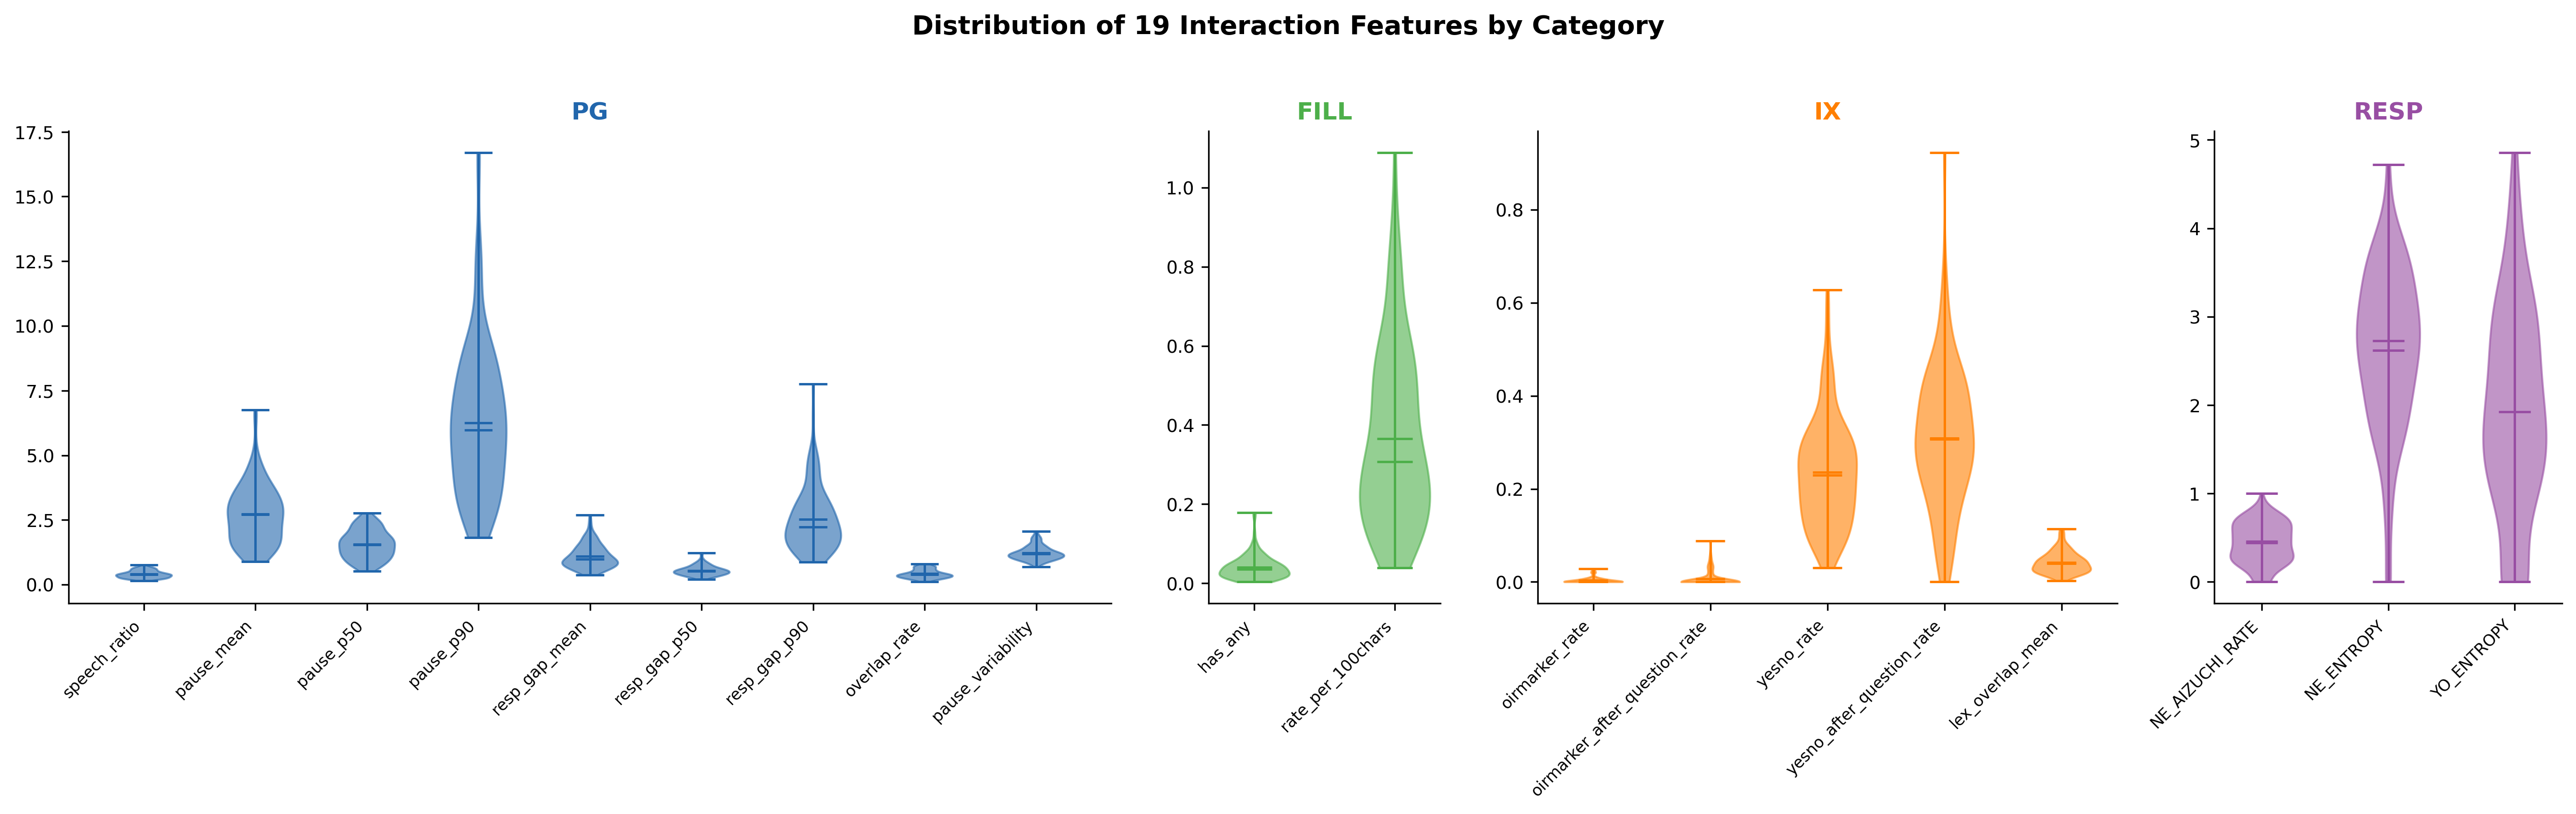
\includegraphics[width=\linewidth]{fig_feature_distribution.png}
\caption{相互行為特徴量の分布（カテゴリ別）．
PG: タイミング系，FILL: フィラー系，IX: 連鎖組織系，RESP: 応答型系．}
\label{fig:feature_dist}
\end{figure}

% [NOTE] 歪度を示していないにも関わらず「正の歪度」と言うのは違和感があったため調整しました．

概ね多くの特徴量について，平均値に対して十分な標準偏差を有するため，幅広い範囲で
特徴量がばらつくことが示された．例えば，PG系指標について，PG\_pause\_mean: $M =
2.702$, $SD = 1.134$, $Min = 0.889$, $Max = 6.761$であり，参加者ごとに多様な値を
取りうることがわかる．PG系指標に限らずFILL系指標（e.g., FILL\_has\_any: $M =
0.040$, $SD = 0.030$）やRESP系指標（e.g., RESP\_NE\_AIZUCHI\_RATE: $M = 0.441$,
$SD = 0.229$），IX系指標（e.g., IX\_yesno\_rate: $M = 0.235$, $SD = 0.115$）も同
様の傾向が確認された．

いくつかの指標は分布が偏る傾向を示した．例えば，PG\_pause\_p90は中央値が平均値よ
り低く高値側に裾を引く分布を示した（$M = 6.253$, $p50 = 5.966$）．同様にFILL系特
徴量も類似の傾向を示した（e.g., FILL\_rate\_per\_100chars: $M = 0.365$, $p50 =
0.308$）．特に，IX系特徴量のうち，OIR関連指標にて強く偏った分布が観察された．すなわ
ち，IX\_oirmarker\_rate （$Min = 0.000$, $p50 = 0.000$）,
IX\_oirmarker\_after\_question\_rate （$Min = 0.000$, $p50 = 0.000$）は大半の話
者でゼロまたは極めて低い値を示し，分布は低値に集中していた．

% [山下6/22適用]#13=B: OIR二値性の記述文を削除（考察3.6節で言及済み）．

なお，RESP系3変数（RESP\_NE\_AIZUCHI\_RATE, RESP\_NE\_ENTROPY, RESP\_YO\_ENTROPY）
は，欠損値が生じ有効$N$が少なくなっているが，これは分母となる終助詞ペアが
存在しない話者が存在するためである．

全体として，相互行為特徴量の多くは個人差を捉えるのに十分なばらつきを示しており，
相互行為の定量化指標として有用であることが確認された．ただし，OIR関連指標のよう
に分布が極端に偏る特徴量については，解釈上の注意が必要だと考えられる．


%% --- 3.2 相関分析 ---
\subsection{相関分析}
\label{sec:result_correlation}

相互行為特徴量間のPearson相関係数を図\ref{fig:corr_heatmap}に示す．具体的な相関
係数の値は\ref{sec:supp_corr}に掲載した．

\begin{figure}[htbp]
\centering
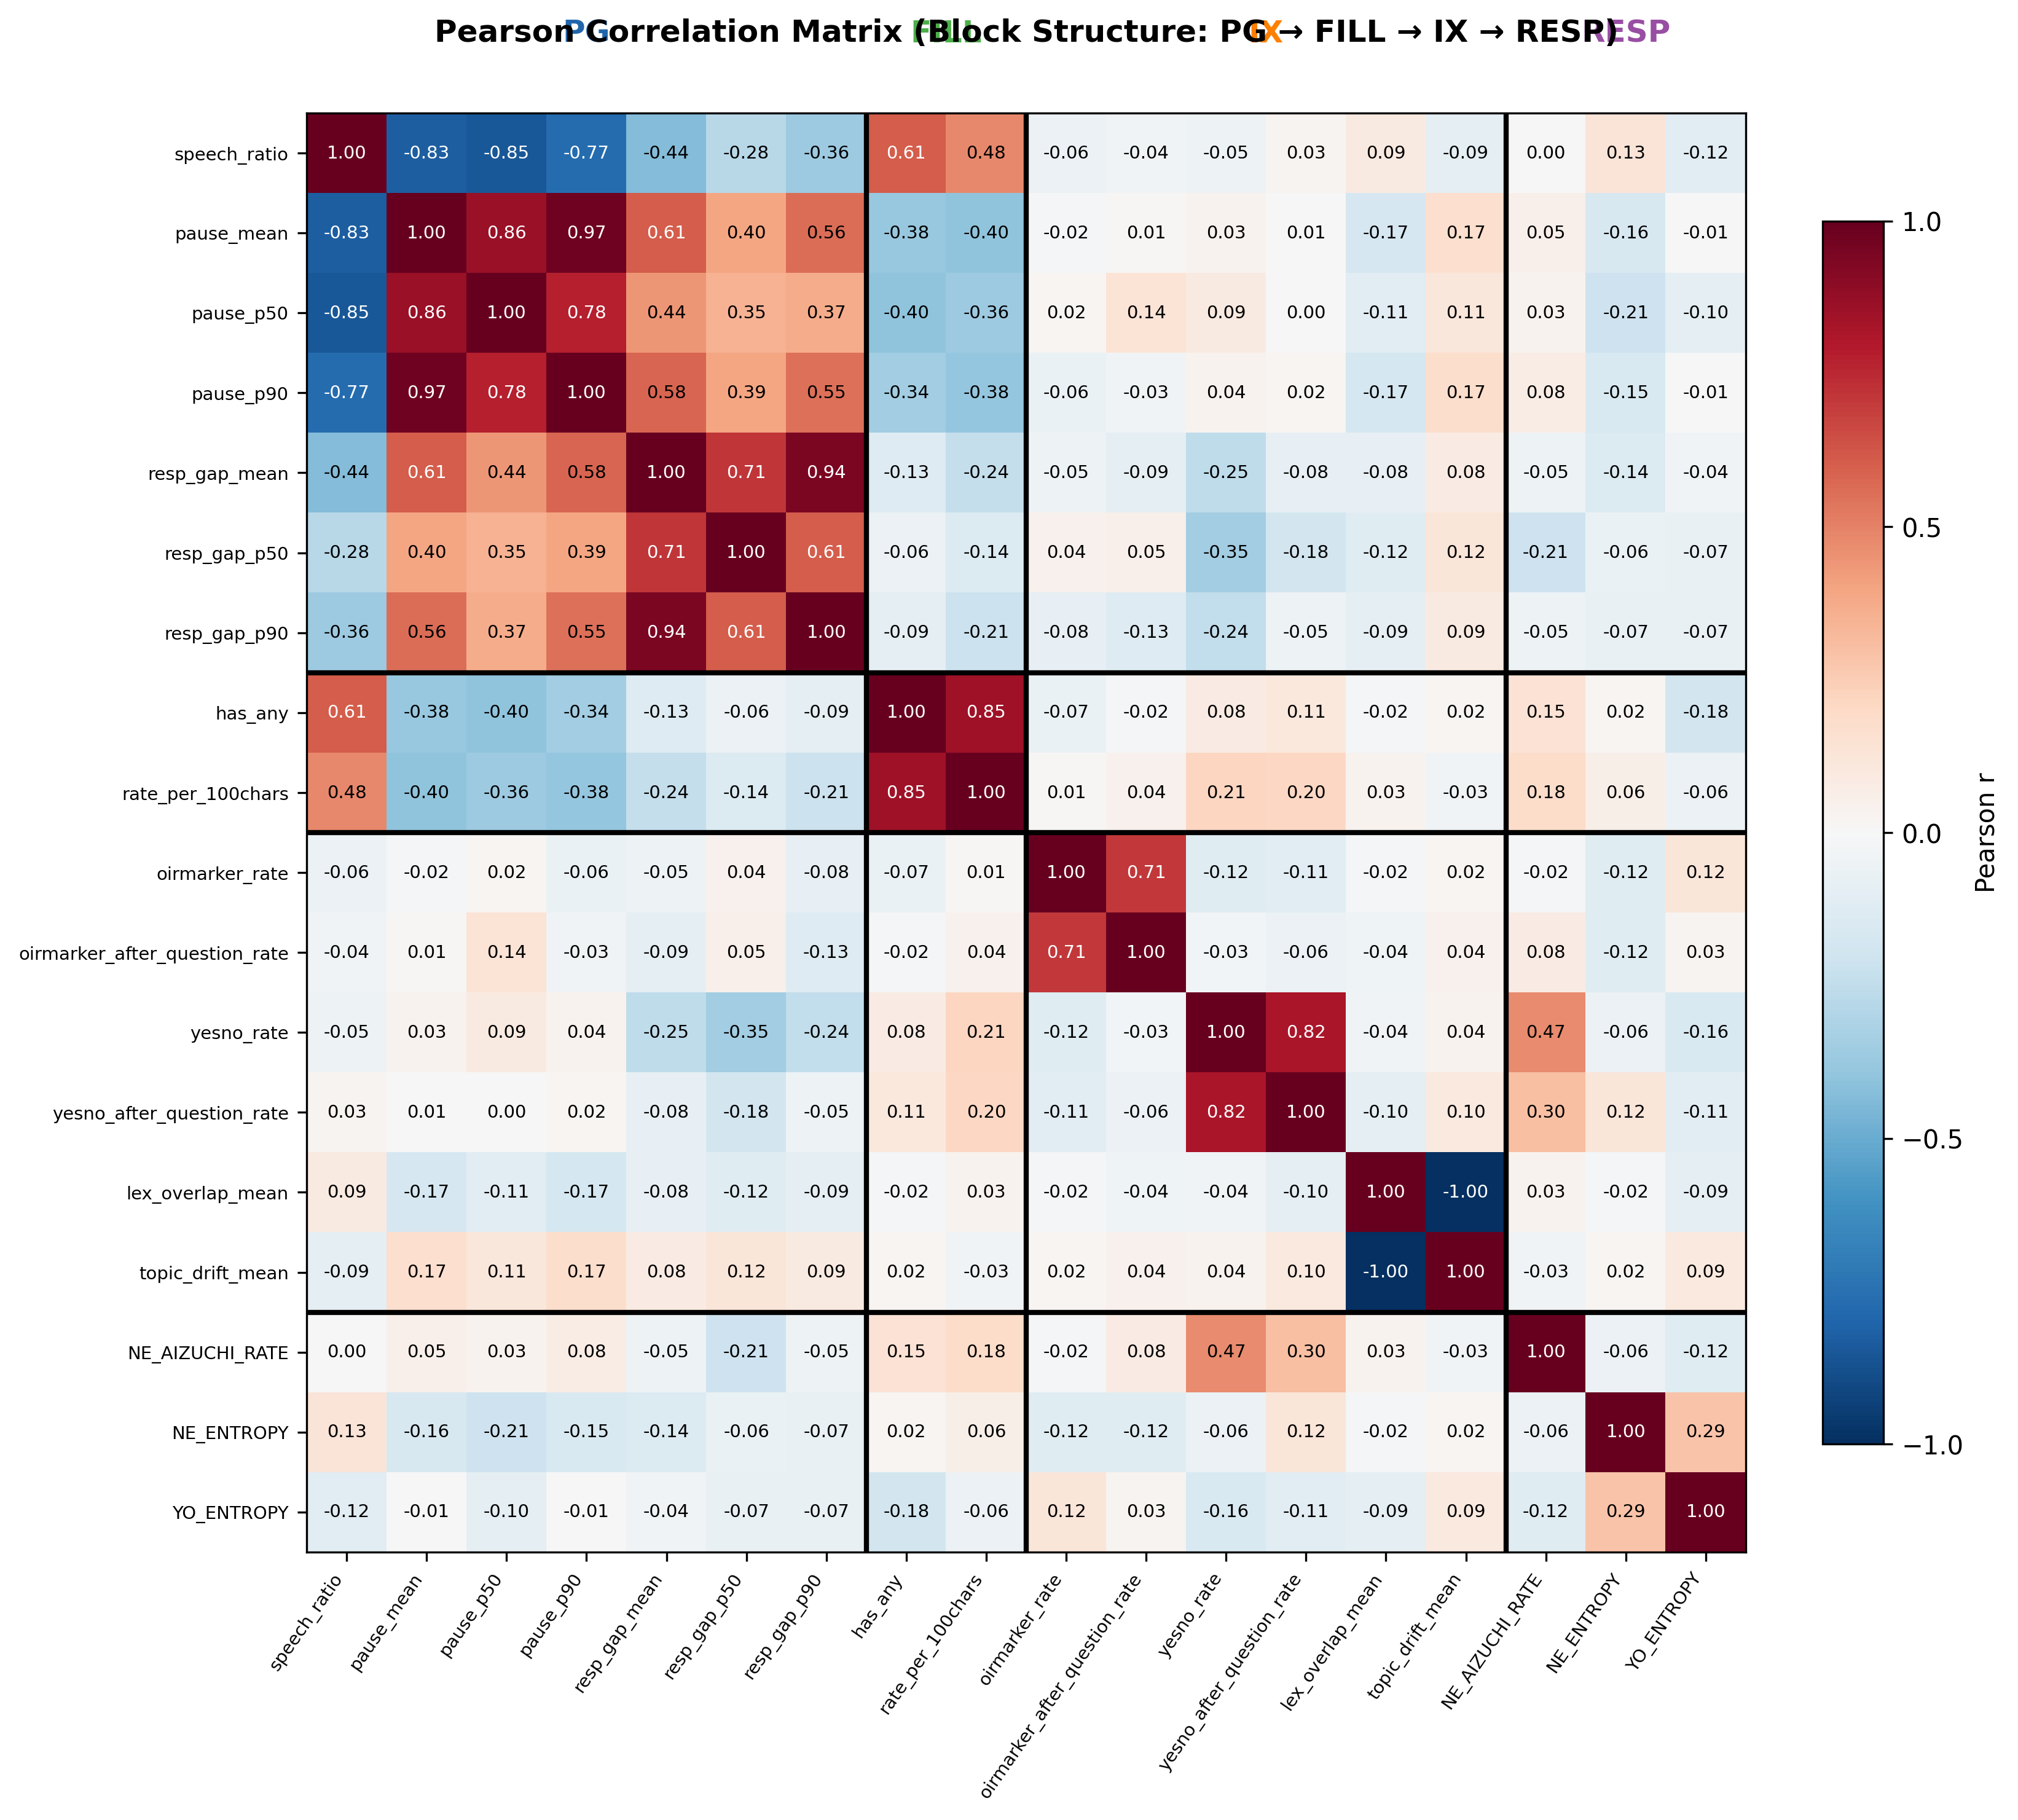
\includegraphics[width=0.95\linewidth]{fig_corr_heatmap_block.png}
\caption{特徴量間相関行列のヒートマップ．実線はカテゴリ境界を示す．}
\label{fig:corr_heatmap}
\end{figure}

PG系特徴量では，沈黙系指標間（PG\_pause\_mean / PG\_pause\_p50 / PG\_pause\_p90）
に$r = 0.78$--$0.97$の高い正の相関が認められた．これらは同一の構成概念（話者内沈
黙の長さ）の異なる集約統計量であり，高い相関は理論的に整合する．同様に，応答遅れ
系指標間（PG\_resp\_gap\_mean / PG\_resp\_gap\_p50 / PG\_resp\_gap\_p90）にも$r
= 0.61$--$0.94$の高い相関が認められた．PG\_speech\_ratio（発話率）は沈黙系指標と
強い負の相関（$r = -0.77$〜$-0.85$）を示し，発話率が高い話者ほど沈黙が短いという
直感的な関係が確認された．

FILL系特徴量では，FILL\_has\_any（フィラー出現発話率）と
FILL\_rate\_per\_100chars（100文字あたりフィラー率）の間に$r = 0.85$の高い相関が
認められた．両指標はフィラー使用の異なる正規化方法であり，高い相関は妥当である．

IX系特徴量では，IX\_oirmarker\_rateとIX\_oirmarker\_after\_question\_rateの間に
$r = 0.71$の相関が認められた．IX\_yesno\_rateとIX\_yesno\_after\_question\_rate
の間にも$r = 0.82$の高い相関があり，全応答と質問直後応答で類似した傾向を示す．

RESP系特徴量では，RESP\_NE\_ENTROPYとRESP\_YO\_ENTROPYの間に$r = 0.29$の弱い正の相関が
認められた程度であり，3変数間の相関は全体的に低い．

カテゴリ間の相関は概ね低く（$|r| < 0.30$），4つのカテゴリが相互に独立した側面を
捉えていることが示された．例外として，PG\_speech\_ratioとFILL\_has\_anyの間に$r
= 0.61$のやや高い正の相関が認められた．これは，発話率の高い話者ほどフィラーを含
む発話が多いことを反映しており，発話量の多さがフィラー出現機会を増やすという解釈
が可能である．


%% --- 3.3 コーパス基本情報との関連性 ---
\subsection{属性情報との関連}
\label{sec:result_metadata}

特徴量の妥当性を外部指標から検証するため，コーパスに付随する人口統計学的属性情報
（性別・年齢）と相互行為特徴量の関連を分析した（表\ref{tab:metadata_tests}）．性
別ごとの分布や年齢の散布図の詳細は，\ref{sec:appendix_metadata}の図\ref{fig:metadata_gender}・図
\ref{fig:metadata_age}に示した．

% [NOTE] 重複する情報，方法に関する情報は極力結果に記述しないようにしてください．

\begin{table}[htbp]
\centering
\caption{相互行為特徴量とコーパス基本情報（性別・年齢）の関連．* $p < 0.05$}
\label{tab:metadata_tests}
{\small
\begin{tabular}{lrrrrrr}
\toprule
Feature & $U$ & $p_{\text{gender}}$ & $r_{\text{Pearson}}$ & $p_{\text{Pearson}}$ & $\rho_{\text{Spearman}}$ & $p_{\text{Spearman}}$ \\
\midrule
PG\_speech\_ratio & \textbf{950} & \textbf{0.0000*} & \textbf{0.455} & \textbf{0.0000*} & \textbf{0.447} & \textbf{0.0000*} \\
PG\_pause\_mean & \textbf{2645} & \textbf{0.0000*} & \textbf{-0.332} & \textbf{0.0002*} & \textbf{-0.389} & \textbf{0.0000*} \\
PG\_pause\_p50 & \textbf{2740} & \textbf{0.0000*} & \textbf{-0.436} & \textbf{0.0000*} & \textbf{-0.449} & \textbf{0.0000*} \\
PG\_pause\_p90 & \textbf{2647} & \textbf{0.0000*} & \textbf{-0.275} & \textbf{0.0024*} & \textbf{-0.343} & \textbf{0.0001*} \\
PG\_resp\_gap\_mean & 1814 & 0.8680 & \textbf{-0.238} & \textbf{0.0087*} & \textbf{-0.241} & \textbf{0.0080*} \\
PG\_resp\_gap\_p50 & 1758 & 0.9034 & \textbf{-0.289} & \textbf{0.0013*} & \textbf{-0.256} & \textbf{0.0047*} \\
PG\_resp\_gap\_p90 & 1812 & 0.8763 & \textbf{-0.212} & \textbf{0.0204*} & \textbf{-0.200} & \textbf{0.0285*} \\
PG\_overlap\_rate & 1518 & 0.1653 & \textbf{0.509} & \textbf{0.0000*} & \textbf{0.500} & \textbf{0.0000*} \\
FILL\_has\_any & \textbf{1406} & \textbf{0.0476*} & \textbf{0.445} & \textbf{0.0000*} & \textbf{0.442} & \textbf{0.0000*} \\
FILL\_rate\_per\_100chars & 1435 & 0.0676 & \textbf{0.415} & \textbf{0.0000*} & \textbf{0.391} & \textbf{0.0000*} \\
IX\_oirmarker\_rate & 1650 & 0.4436 & -0.104 & 0.2592 & -0.105 & 0.2549 \\
IX\_oirmarker\_after\_question\_rate & 1952 & 0.2091 & -0.076 & 0.4093 & -0.102 & 0.2699 \\
IX\_yesno\_rate & 1860 & 0.6846 & \textbf{0.252} & \textbf{0.0055*} & \textbf{0.249} & \textbf{0.0060*} \\
IX\_yesno\_after\_question\_rate & 1716 & 0.7317 & \textbf{0.296} & \textbf{0.0010*} & \textbf{0.279} & \textbf{0.0020*} \\
IX\_lex\_overlap\_mean & \textbf{1109} & \textbf{0.0004*} & -0.115 & 0.2116 & -0.126 & 0.1706 \\
RESP\_NE\_AIZUCHI\_RATE & 1643 & 0.9528 & \textbf{0.272} & \textbf{0.0033*} & \textbf{0.289} & \textbf{0.0017*} \\
RESP\_NE\_ENTROPY & 1546 & 0.6321 & 0.030 & 0.7542 & 0.059 & 0.5286 \\
RESP\_YO\_ENTROPY & 1839 & 0.5495 & -0.087 & 0.3482 & -0.027 & 0.7685 \\
PG\_pause\_variability & 1736 & 0.8103 & -0.023 & 0.8007 & -0.039 & 0.6712 \\
\bottomrule
\end{tabular}
}

\end{table}

% [NOTE] テーブルについて太字で有意を示すジャーナルは少ないのでアスタリスクで統一しましょう

7つの特徴量で有意な性差が認められた．
PG系タイミング指標では，PG\_speech\_ratio（$U = 950$, $p < 0.0001$），
PG\_pause\_mean（$U = 2645$, $p < 0.0001$），
PG\_pause\_p50（$U = 2740$, $p < 0.0001$），
PG\_pause\_p90（$U = 2647$, $p < 0.0001$）は有意差が認められ，
女性の方が発話率が高く沈黙が短い傾向を示した．
FILL\_has\_any（$U = 1406$, $p = 0.048$）は女性の方がフィラー出現発話率が高かった．
IX系では，IX\_lex\_overlap\_mean（$U = 1109$, $p = 0.0004$）は女性の方が語彙重なりが高く，
IX\_topic\_drift\_mean（$U = 2455$, $p = 0.0004$）は男性の方が話題逸脱度が高かった．
% [山下6/22適用] #14=C: 性差の解釈は考察（コーパス基本情報との関連の解釈）に移動済みのため，結果節からは数値のみ残し解釈文を削除．

12の特徴量が年齢と有意に相関した．
PG\_speech\_ratio（$\rho = 0.447$, $p < 0.0001$）は年齢と，相対的に強い正の相関を示し，
年齢が高い話者ほど発話率が高い傾向が確認された．
沈黙系指標（PG\_pause\_mean: $\rho = -0.389$; PG\_pause\_p50: $\rho = -0.449$;
PG\_pause\_p90: $\rho = -0.343$）および応答遅れ系指標
（PG\_resp\_gap\_mean: $\rho = -0.241$; PG\_resp\_gap\_p50: $\rho = -0.256$;
PG\_resp\_gap\_p90: $\rho = -0.200$）は年齢と有意な負の相関を示し，
年齢が高い話者ほど沈黙・応答遅れが短い傾向が認められた．
FILL系指標（FILL\_has\_any: $\rho = 0.442$; FILL\_rate\_per\_100chars: $\rho = 0.391$）は
年齢と強い正の相関を示し，年齢が高い話者ほどフィラー使用が多い傾向が確認された．
IX系では，IX\_yesno\_rate（$\rho = 0.249$）およびIX\_yesno\_after\_question\_rate（$\rho = 0.279$）が
年齢と有意な正の相関を示し，年齢が高い話者ほどYES/NO応答が多い傾向が認められた．
RESP\_NE\_AIZUCHI\_RATE（$\rho = 0.289$, $p = 0.002$）も年齢と有意な正の相関を示し，
年齢が高い話者ほど「ね」直後の相槌が多い傾向が確認された．

相互行為特徴量のうち12特徴量が年齢と，7特徴量が性別と有意な関連を示した．
特にPG系（タイミング）とFILL系（フィラー）は性別・年齢の両方と比較的強い関連を持っていた．
特徴量が話者の属性（性別・年齢）という外部指標と体系的に関連することは，
これらの指標が話者の個人差を捉えていることを示唆している．

% [NOTE] 表面的妥当性の使い方に違和感があるので削除にしましょう

\subsection{性格特性との関連}
\label{sec:result_big5}

% [NOTE] 方法と重複があるので，冒頭のメソッドの説明は最低限で良いと思います．また表面的妥当性・構成概念妥当性の使い方に違和感があるので，削除でOKです．
% [NOTE] このセクションの結果については，全体で先に相談した方がよいかと思いましたので，ほとんど手をつけておりません．

相互行為特徴量の有用性を裏付けるために，相互行為特徴量が心理学的に意味のある個人
差次元（Big5性格特性）と関連するかどうかを検証した．具体的には，4つのLLMモデ
ルの自己報告式質問紙（IPIP-NEO-120）に対する回答から仮想Big5スコアを算出し，これ
を外的基準とした．新しく提案した相互行為特徴量の追加効果を検証するため，説明変数
を3段階で構成する段階的なRidge回帰分析を実施した．

表\ref{tab:three_stage}および図\ref{fig:three_stage}に，全5次元の3段階比較結果を示す．

% [山下6/22適用] 主指標を相関rから増分妥当性R²・予測誤差RMSEへ変更．

\begin{table}[htbp]
\centering
\caption{3段階Ridge回帰比較（OOF-pooled $R^2$ / RMSE）．Stage 1: 人口統計のみ（2変数），
Stage 2: +Classical（12変数），Stage 3: +Novel（21変数）．
$\Delta R^2$・$\Delta\text{RMSE}$は隣接ステージ間の増分を示す．
Stage 2→3（Novel追加）の増分に付した記号は，レコード単位OOF二乗誤差のpaired bootstrap検定
（$^{*}$: $p<0.05$，$^{\mathrm{ns}}$: 有意でない）を表す．}
\label{tab:three_stage}
\begin{tabular}{llrcccc}
\toprule
Trait & Stage & $n_{feat}$ & $R^2_{oof}$ & RMSE & $\Delta R^2$ & $\Delta$RMSE \\
\midrule
O & Demographics & 2 & 0.064 & 0.327 & --- & --- \\
 & +Classical & 12 & 0.193 & 0.304 & +0.129 & -0.023 \\
 & +Novel & 21 & 0.206 & 0.301 & +0.013$^{\mathrm{ns}}$ & -0.003$^{\mathrm{ns}}$ \\
\midrule
C & Demographics & 2 & 0.128 & 0.394 & --- & --- \\
 & +Classical & 12 & 0.146 & 0.390 & +0.018 & -0.004 \\
 & +Novel & 21 & 0.196 & 0.379 & +0.049$^{\mathrm{ns}}$ & -0.011$^{\mathrm{ns}}$ \\
\midrule
E & Demographics & 2 & -0.015 & 0.345 & --- & --- \\
 & +Classical & 12 & 0.067 & 0.331 & +0.082 & -0.014 \\
 & +Novel & 21 & 0.025 & 0.339 & -0.043$^{*}$ & +0.007$^{*}$ \\
\midrule
A & Demographics & 2 & 0.196 & 0.231 & --- & --- \\
 & +Classical & 12 & 0.223 & 0.227 & +0.027 & -0.004 \\
 & +Novel & 21 & 0.253 & 0.222 & +0.031$^{\mathrm{ns}}$ & -0.004$^{\mathrm{ns}}$ \\
\midrule
N & Demographics & 2 & 0.009 & 0.362 & --- & --- \\
 & +Classical & 12 & 0.021 & 0.360 & +0.011 & -0.002 \\
 & +Novel & 21 & 0.061 & 0.353 & +0.040$^{\mathrm{ns}}$ & -0.007$^{\mathrm{ns}}$ \\
\bottomrule
\end{tabular}

\end{table}

\begin{figure}[htbp]
\centering
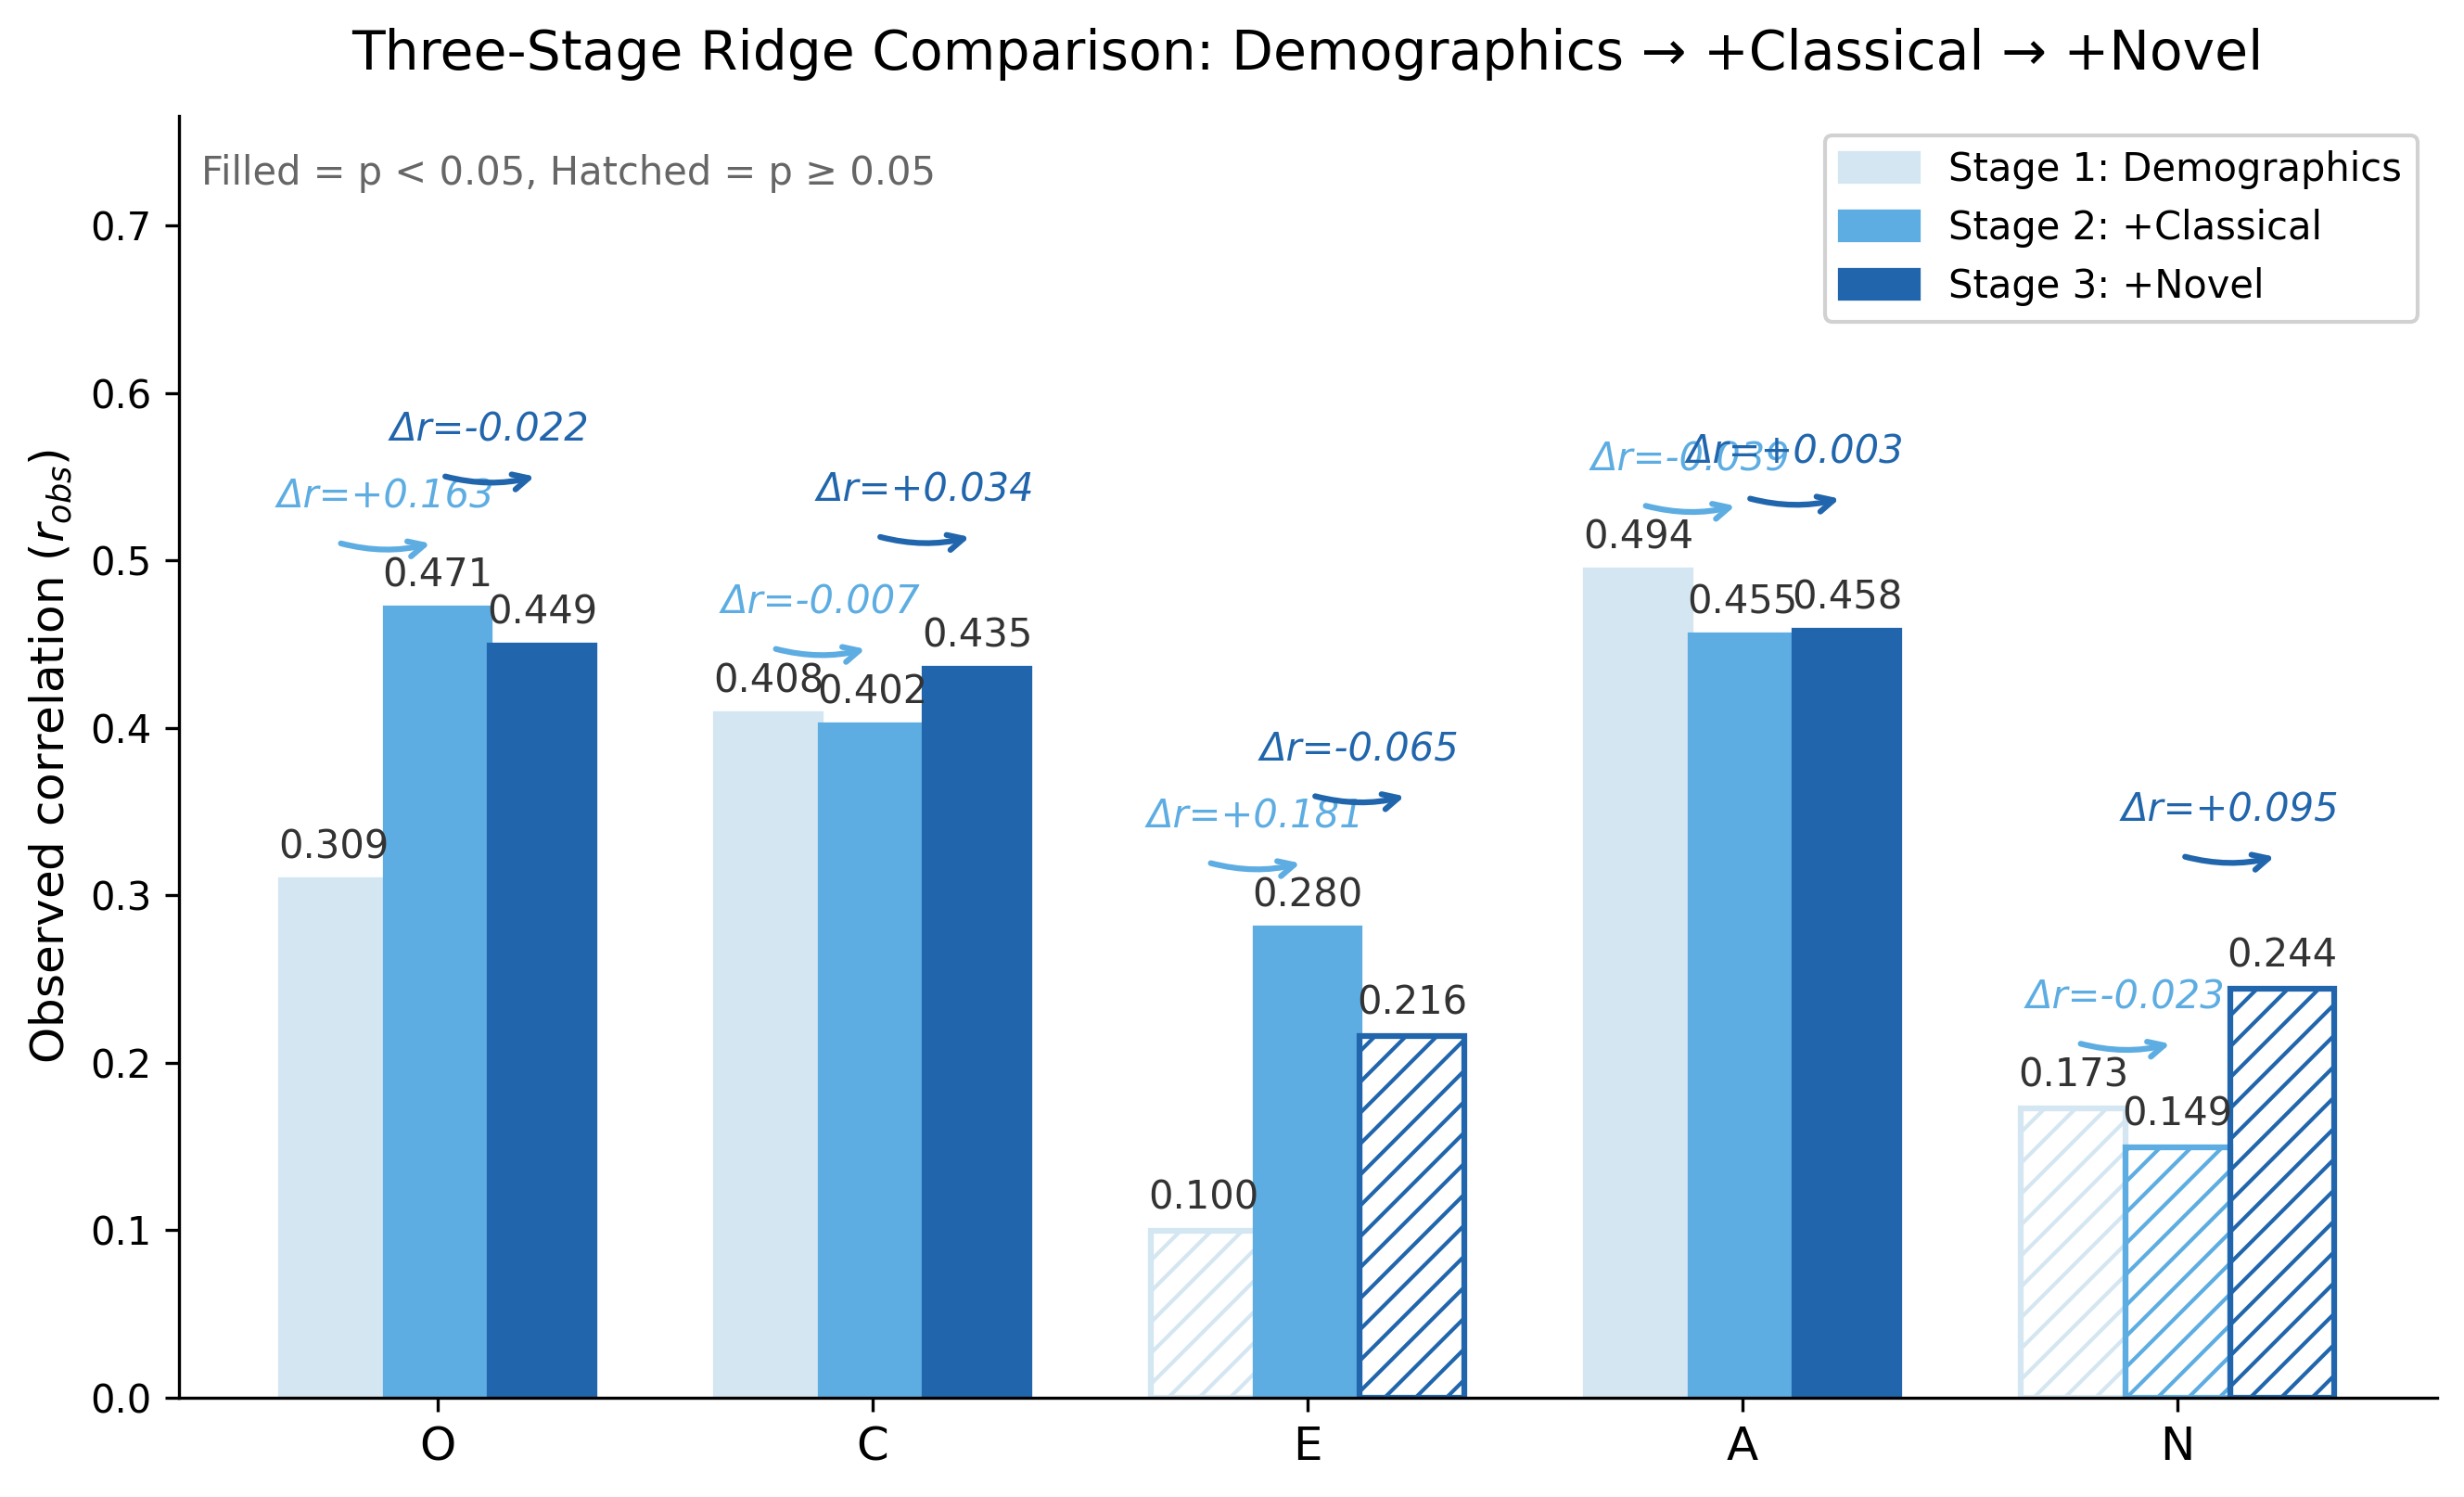
\includegraphics[width=0.9\linewidth]{fig_three_stage_comparison.png}
\caption{3段階Ridge回帰比較（全5次元，OOF-pooled $R^2$）．
各次元についてStage 1（人口統計のみ），Stage 2（+Classical），
Stage 3（+Novel）の$R^2_{\text{oof}}$を並列表示し，$\Delta R^2$を付記．
Stage 2→3の増分にはpaired bootstrap検定の結果（$^{*}$: $p<0.05$，n.s.: 有意でない）を併記した．}
\label{fig:three_stage}
\end{figure}

人口統計変数のみのStage 1に対して，古典的特徴量（PG系タイミング指標・FILL系フィラー指標）を
追加したStage 2では，全次元で$R^2_{\text{oof}}$の向上が認められた．
向上幅はEで最大（$\Delta R^2 = +0.115$，$R^2$: $-0.017 \to 0.098$，RMSE: $0.346 \to 0.326$）で，
Oがこれに次いだ（$+0.107$，$0.037 \to 0.144$）．
C（$+0.056$，$0.077 \to 0.133$），N（$+0.037$，$-0.027 \to 0.010$），
A（$+0.029$，$0.112 \to 0.140$）も一貫して上昇し，
タイミング・フィラー系の古典的特徴量が予測に寄与することが確認された．

古典的特徴量に加えて新規特徴量（IX系連鎖組織指標・RESP系応答型指標）を
追加したStage 3では，5次元中3次元（O・C・N）で$R^2_{\text{oof}}$が上昇し，RMSEが低下した
（N: $\Delta R^2 = +0.069$，C: $+0.048$，O: $+0.010$）．
一方，E（$\Delta R^2 = -0.026$）とA（$-0.014$）では小幅な低下がみられた．
なお，相関$r$による集計（\ref{sec:appendix_three_stage_r}）ではOの増分が負に転じるが，
$R^2$・RMSEでは改善側に評価される．これは新規特徴量が順位的一致を大きく変えなくても
予測値のキャリブレーションを改善しうることを示唆する．
paired bootstrap検定では，名目的に有意な増分はNのみであった
（$\Delta R^2 = +0.069$，$p_{\text{boot}} = 0.044$）．
ただしこの増分はWilcoxon符号付順位検定では有意でなく（$p = 0.19$），頑健とは言えない．
他の4次元（O・C・E・A）はいずれも有意でなく（$p_{\text{boot}} = 0.10$--$0.72$），
統計的に有意な悪化も認められなかった．

総じて，新規特徴量（IX系・RESP系）の追加は，大部分の次元で予測を劣化させない
ものの，モデル全体の増分としては頑健な予測改善を示すには至らなかった．

% [NOTE] 以下は考察に近い内容（加えて前後に脈絡のない内容だったので）なので削除しました
% > 新規特徴量の実質的な寄与は，モデル全体の増分ではなく個別特徴量の係数レベルで評価することが適切であり，


最終的にStage 3において構築されたリッジ回帰モデルを用いた予測値の散布図（図
\ref{fig:predicted_vs_observed}）ならびに置換検定の結果（表
\ref{tab:ensemble_perm}）を示す．Holm法の補正の有無に限らず，5次元中4次元（O, C,
A, N）で相互行為特徴量との有意な関連が認められた．具体的には，Agreeableness（A）が$r = 0.449$（$p = 0.0004$, $p_{\text{corrected}} = 0.0020$）と5次元中
で最も高い予測精度を示した．Conscientiousness（C）が$r = 0.432$（$p =
0.0006$, $p_{\text{corrected}} = 0.0024$）でこれに次いだ．Openness（O，
$r = 0.410$, $p = 0.0014$, $p_{\text{corrected}} = 0.0042$），Neuroticism（N，
$r = 0.317$, $p = 0.0122$, $p_{\text{corrected}} = 0.0244$）も有意であっ
た．Extraversion（E）のみ補正前・補正後ともに有意水準に達しなかった（$r
= 0.234$, $p = 0.0658$, $p_{\text{corrected}} = 0.0658$）．

\begin{table}[htbp]
\centering
\caption{仮想Big5に対する置換検定結果（全5次元）．
観測相関係数$r_{\text{obs}}$，補正前$p$値，およびHolm法による補正後$p$値を示す．$^{*}$は補正後$p < 0.05$（有意）．}
\label{tab:ensemble_perm}
\begin{tabular}{lcc}
\toprule
Trait & $r_{obs}$ & $p$-value \\
\midrule
O & \textbf{0.360} & \textbf{0.0048} \\
C & \textbf{0.447} & \textbf{0.0004} \\
E & 0.217 & 0.0902 \\
A & \textbf{0.465} & \textbf{0.0004} \\
N & \textbf{0.309} & \textbf{0.0152} \\
\bottomrule
\end{tabular}

\end{table}

\begin{figure}[htbp]
\centering
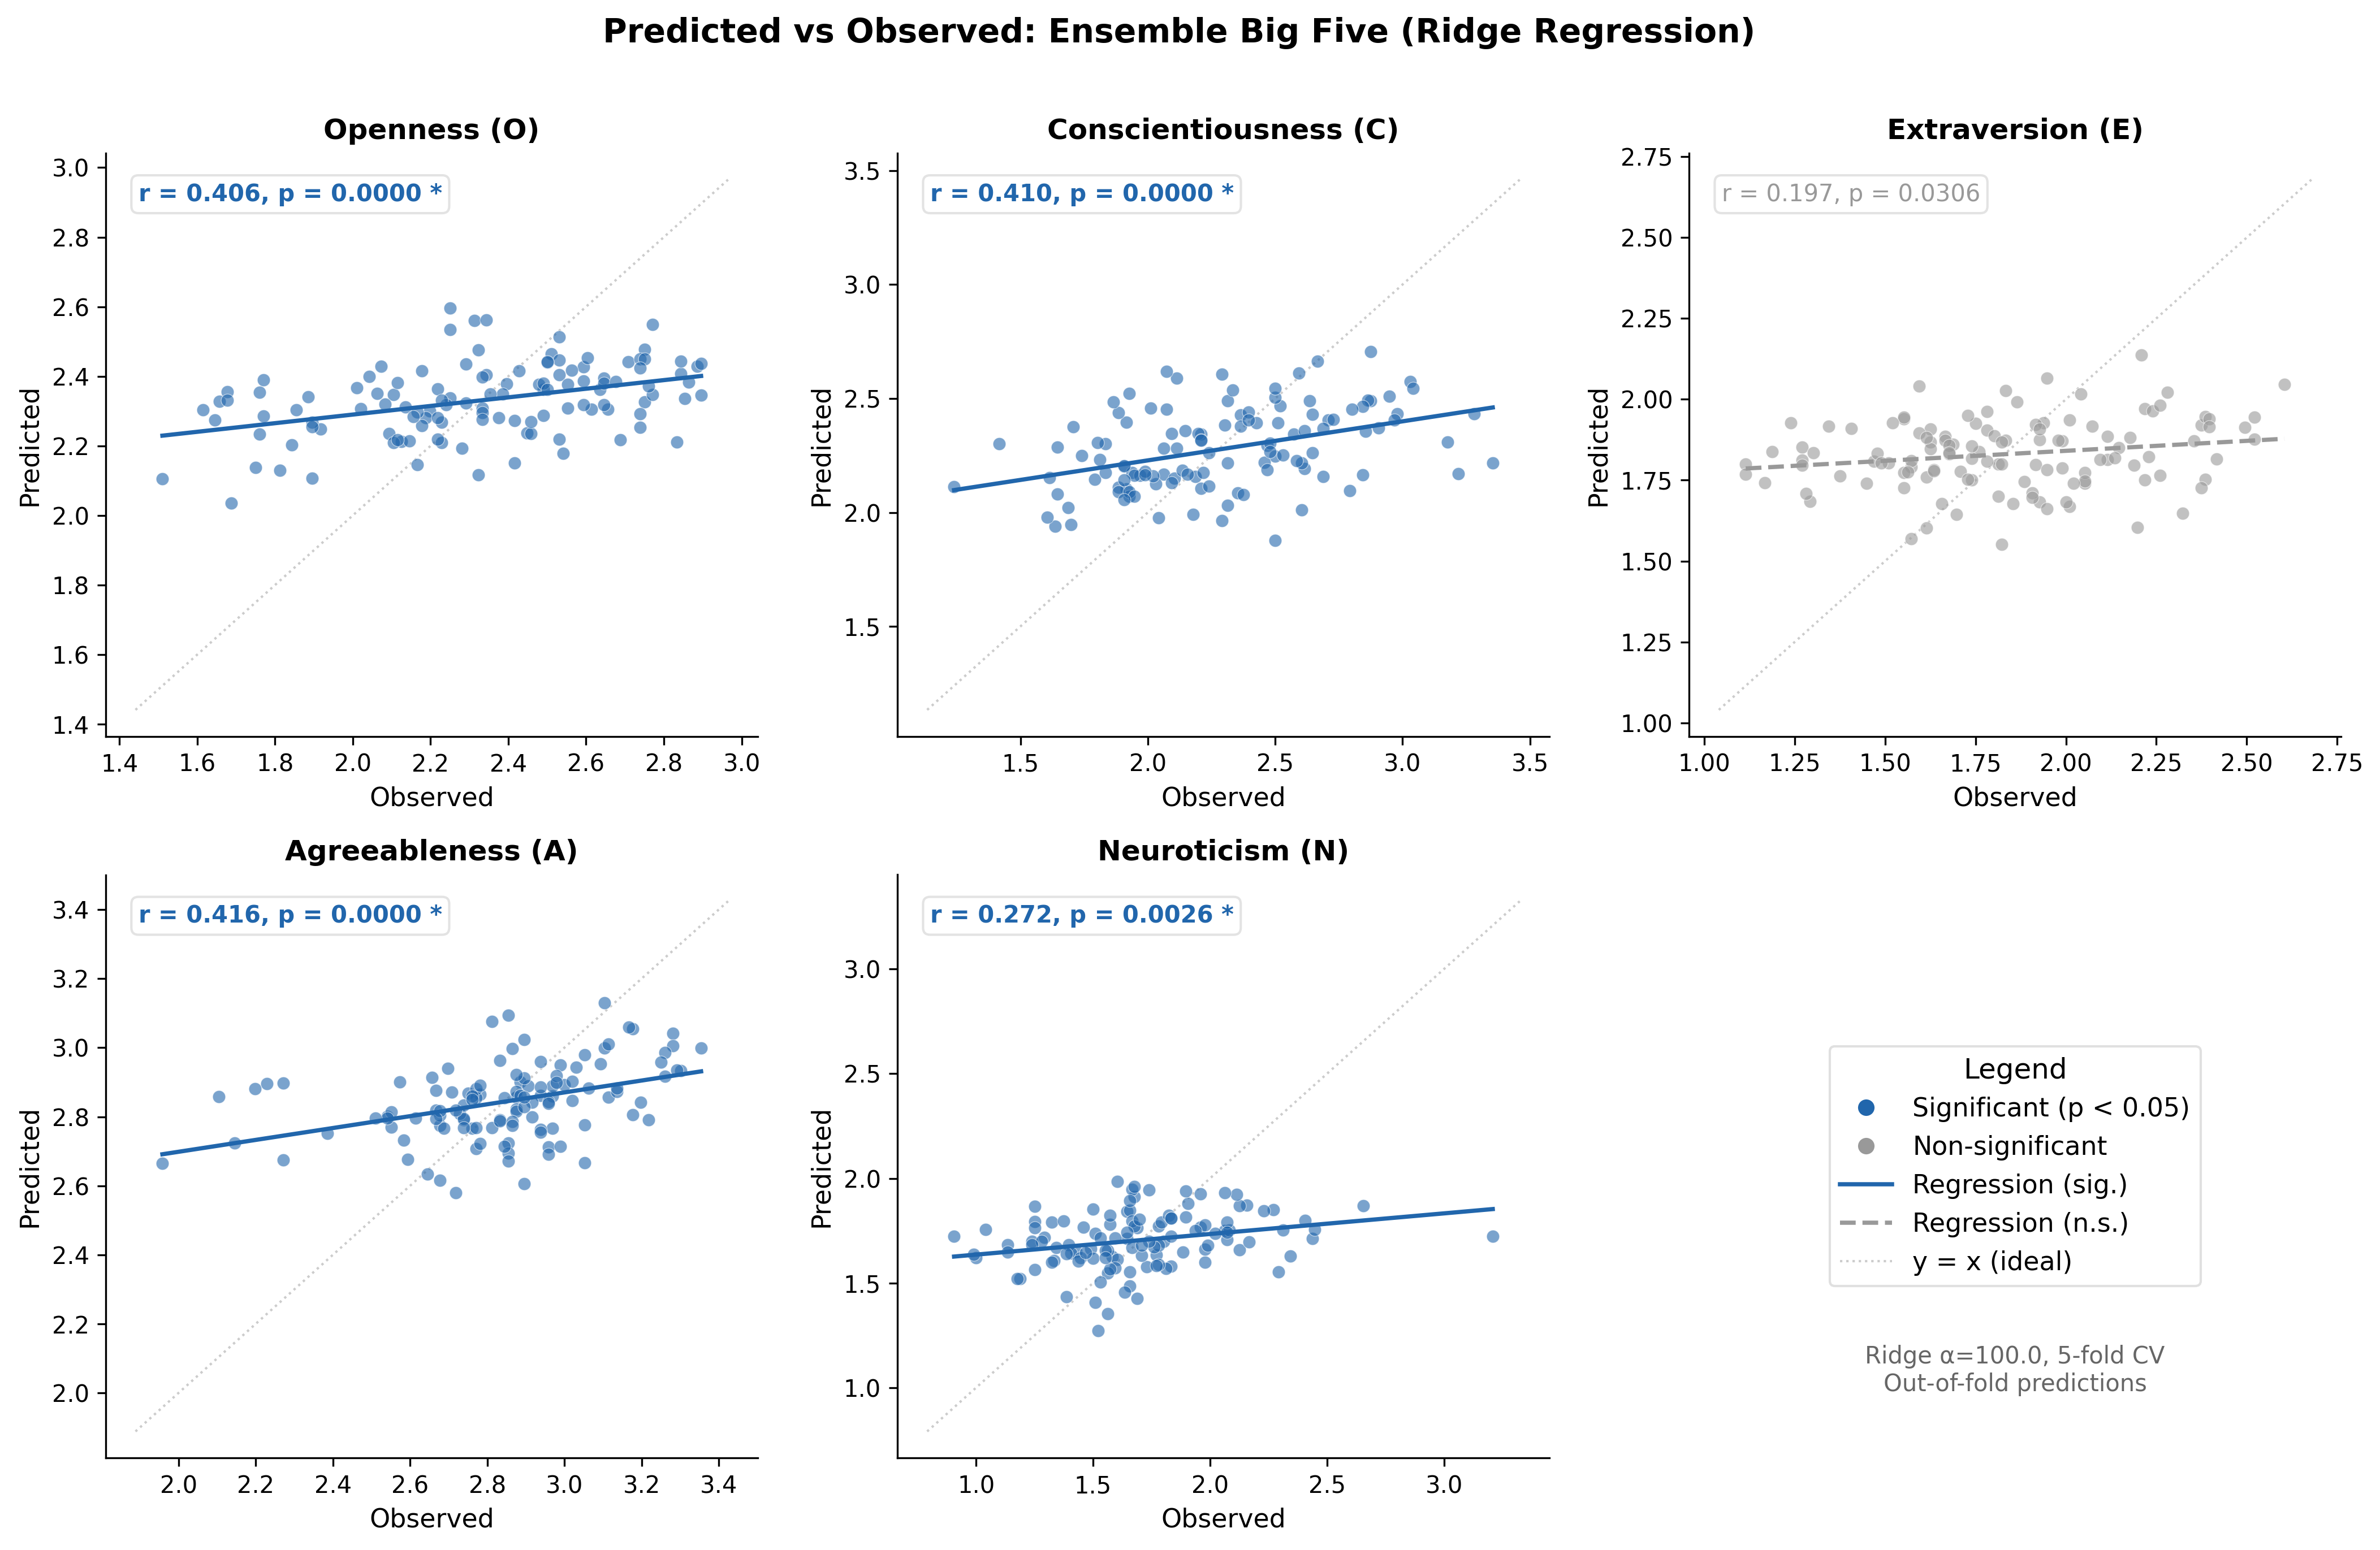
\includegraphics[width=0.9\linewidth]{fig_predicted_vs_observed.png}
\caption{仮想Big5の予測値 vs 観測値散布図（全5次元）．
各点は1レコード（会話$\times$話者ペア）を表す．
横軸は観測値（仮想Big5スコア），縦軸はRidge回帰のout-of-fold予測値．
実線は回帰直線，破線は$y = x$の参照線．
各パネルにPearson $r$および$p$値を付記．
有意な次元（O, C, A, N）は青色，非有意な次元（E）はグレーで表示．}
\label{fig:predicted_vs_observed}
\end{figure}

\ref{sec:appendix_individual_teacher}には，LLMモデル間の平均ではなくLLMモデルごとの結果を報告する．

% [NOTE] 短い論文において下記のような導入向けの記載は不要です．
% > 次節（3.4.4節）のPermutation回帰係数検定では，Classical・Novel両群から誠実性（C）の予測に有意な特徴量が同定される．





\subsection{性格特性の予測に重要な相互行為特徴量}
\label{sec:xai_analysis}

\subsubsection{置換検定}
\label{sec:result_permutation_coef}

% [NOTE] 説明が冗長だったので大きく削除しました．
% [NOTE] この結果はCだけ選択しているようですが，どのような根拠でしたでしょうか．Cが最も安定しているためという記述が散見されましたが，結果を拝見する限りあまり強い主張はできないような印象があります．Cだけをセレクトせずにすべての結果を載せるのは如何でしょうか．また全体でディスカッションして決めたいので一旦保留で大丈夫です．

表\ref{tab:permutation_coef}に，リッジ回帰モデルの回帰係数の置換検定の結果を示す．
単一のLLMモデルを用いた予備的解析より，CはLLMモデルに依存しない安定した結果を示すことが明らかとなった
（\ref{sec:appendix_llm}）．そのため，本文ではCに関する結果を報告する．
仮想Big5のCに対して有意であった特徴量は以下の7個である: PG\_speech\_ratio（発話
率，$\beta = 0.022$, $p = 0.019$），PG\_pause\_mean（平均沈黙長，$\beta =
-0.021$, $p = 0.004$），PG\_pause\_p50（沈黙長中央値，$\beta = -0.025$, $p =
0.006$），PG\_pause\_p90（沈黙長90パーセンタイル，$\beta = -0.022$, $p = 0.010$），
IX\_yesno\_rate（YES/NO応答率，$\beta = 0.022$, $p = 0.022$），
IX\_yesno\_after\_question\_rate（質問直後YES/NO率，$\beta = 0.023$, $p =
0.035$），RESP\_NE\_ENTROPY（「ね」直後応答多様性，$\beta = -0.032$, $p =
0.011$）．有意な特徴量はPG系タイミング指標（4個），IX系相互行為指標（2個），RESP
系応答型指標（1個）にまたがり，古典的特徴量と新規特徴量の両群から同定
された．なお，FILL\_has\_any（$p = 0.779$），
IX\_oirmarker\_after\_question\_rate（$p = 0.510$），IX\_lex\_overlap\_mean（$p
= 0.521$），IX\_topic\_drift\_mean（$p = 0.521$）は有意水準に達しなかった．


\begin{table}[htbp]
\centering
\caption{回帰係数に対する置換検定（Conscientiousness）．
各特徴量の回帰係数$\beta_{\text{obs}}$および$p$値を示す．$^{*}$は$p < 0.05$（有意）．}
\label{tab:permutation_coef}
\begin{tabular}{lrr}
\toprule
Feature & $\beta_{\mathrm{obs}}$ & $p$-value \\
\midrule
PG\_speech\_ratio & 0.0216 & 0.0214$^{*}$ \\
PG\_pause\_mean & -0.0202 & 0.0022$^{*}$ \\
PG\_pause\_p50 & -0.0257 & 0.0022$^{*}$ \\
PG\_pause\_p90 & -0.0218 & 0.0098$^{*}$ \\
PG\_resp\_gap\_mean & 0.0127 & 0.1192 \\
PG\_resp\_gap\_p50 & -0.0089 & 0.4611 \\
PG\_resp\_gap\_p90 & 0.0048 & 0.6217 \\
PG\_overlap\_rate & 0.0020 & 0.8638 \\
FILL\_has\_any & 0.0030 & 0.7602 \\
FILL\_rate\_per\_100chars & 0.0197 & 0.0568 \\
IX\_oirmarker\_rate & 0.0045 & 0.6917 \\
IX\_oirmarker\_after\_question\_rate & -0.0082 & 0.4865 \\
IX\_yesno\_rate & 0.0220 & 0.0224$^{*}$ \\
IX\_yesno\_after\_question\_rate & 0.0225 & 0.0334$^{*}$ \\
IX\_lex\_overlap\_mean & 0.0083 & 0.5181 \\
RESP\_NE\_AIZUCHI\_RATE & 0.0211 & 0.0890 \\
RESP\_NE\_ENTROPY & -0.0319 & 0.0110$^{*}$ \\
RESP\_YO\_ENTROPY & 0.0046 & 0.6999 \\
PG\_pause\_variability & -0.0059 & 0.6193 \\
\bottomrule
\end{tabular}

\end{table}


%% --- 3.4.4b Bootstrap分散ベース安定性分析 ---
\subsubsection{Bootstrap法による安定性分析}
\label{sec:result_bootstrap_variance}

Bootstrap法による各特徴量の回帰係数の標準偏差（SD）および95\%信頼区間（CI）を表
\ref{tab:bootstrap_variance}に，フォレストプロットを図
\ref{fig:bootstrap_variance}に示す．仮想Big5のCに対して95\%CIがゼロを除外した特
徴量は以下の9個である:
PG\_speech\_ratio（$\bar{\beta} = 0.020$, CI $= [0.005, 0.036]$），
PG\_pause\_mean（$\bar{\beta} = -0.021$, CI $= [-0.035, -0.008]$），
PG\_pause\_p50（$\bar{\beta} = -0.025$, CI $= [-0.040, -0.009]$），
PG\_pause\_p90（$\bar{\beta} = -0.022$, CI $= [-0.037, -0.006]$），
FILL\_rate\_per\_100chars（$\bar{\beta} = 0.020$, CI $= [0.002, 0.035]$），
IX\_yesno\_rate（$\bar{\beta} = 0.021$, CI $= [0.005, 0.040]$），
IX\_yesno\_after\_question\_rate（$\bar{\beta} = 0.022$, CI $= [0.004, 0.040]$），
RESP\_NE\_AIZUCHI\_RATE（$\bar{\beta} = 0.021$, CI $= [0.003, 0.040]$），
RESP\_NE\_ENTROPY（$\bar{\beta} = -0.031$, CI $= [-0.054, -0.004]$）．
なお，FILL\_has\_any，IX\_oirmarker\_after\_question\_rate，
IX\_lex\_overlap\_mean，IX\_topic\_drift\_meanは
95\%CIがゼロを跨いでおり，安定的な寄与は確認されなかった．

% [NOTE] 「負の寄与」などは直前の数字を見ればわかるので削除で良いです．

\begin{table}[htbp]
\centering
\caption{各特徴量の平均回帰係数，SD，95\%CI．
$^{*}$はCIがゼロを含まない（有意）ことを示す．}
\label{tab:bootstrap_variance}
\begin{tabular}{lrrrr}
\toprule
Feature & $\bar{\beta}$ & SD & CI$_{2.5}$ & CI$_{97.5}$ \\
\midrule
PG\_speech\_ratio$^{*}$ & 0.0204 & 0.0079 & 0.0045 & 0.0361 \\
PG\_pause\_mean$^{*}$ & -0.0209 & 0.0071 & -0.0347 & -0.0075 \\
PG\_pause\_p50$^{*}$ & -0.0247 & 0.0080 & -0.0402 & -0.0091 \\
PG\_pause\_p90$^{*}$ & -0.0220 & 0.0079 & -0.0366 & -0.0058 \\
PG\_resp\_gap\_mean & 0.0105 & 0.0063 & -0.0019 & 0.0232 \\
PG\_resp\_gap\_p50 & -0.0090 & 0.0077 & -0.0243 & 0.0066 \\
PG\_resp\_gap\_p90 & 0.0028 & 0.0078 & -0.0134 & 0.0171 \\
FILL\_has\_any & 0.0035 & 0.0072 & -0.0093 & 0.0189 \\
FILL\_rate\_per\_100chars$^{*}$ & 0.0195 & 0.0088 & 0.0015 & 0.0353 \\
IX\_oirmarker\_rate & 0.0039 & 0.0110 & -0.0168 & 0.0249 \\
IX\_oirmarker\_after\_question\_rate & -0.0081 & 0.0068 & -0.0209 & 0.0051 \\
IX\_yesno\_rate$^{*}$ & 0.0214 & 0.0088 & 0.0054 & 0.0396 \\
IX\_yesno\_after\_question\_rate$^{*}$ & 0.0215 & 0.0091 & 0.0042 & 0.0400 \\
IX\_lex\_overlap\_mean & 0.0053 & 0.0066 & -0.0078 & 0.0167 \\
IX\_topic\_drift\_mean & -0.0053 & 0.0066 & -0.0167 & 0.0078 \\
RESP\_NE\_AIZUCHI\_RATE$^{*}$ & 0.0214 & 0.0093 & 0.0027 & 0.0402 \\
RESP\_NE\_ENTROPY$^{*}$ & -0.0307 & 0.0124 & -0.0537 & -0.0042 \\
RESP\_YO\_ENTROPY & 0.0034 & 0.0130 & -0.0215 & 0.0284 \\
\bottomrule
\end{tabular}

\end{table}

\begin{figure}[htbp]
\centering
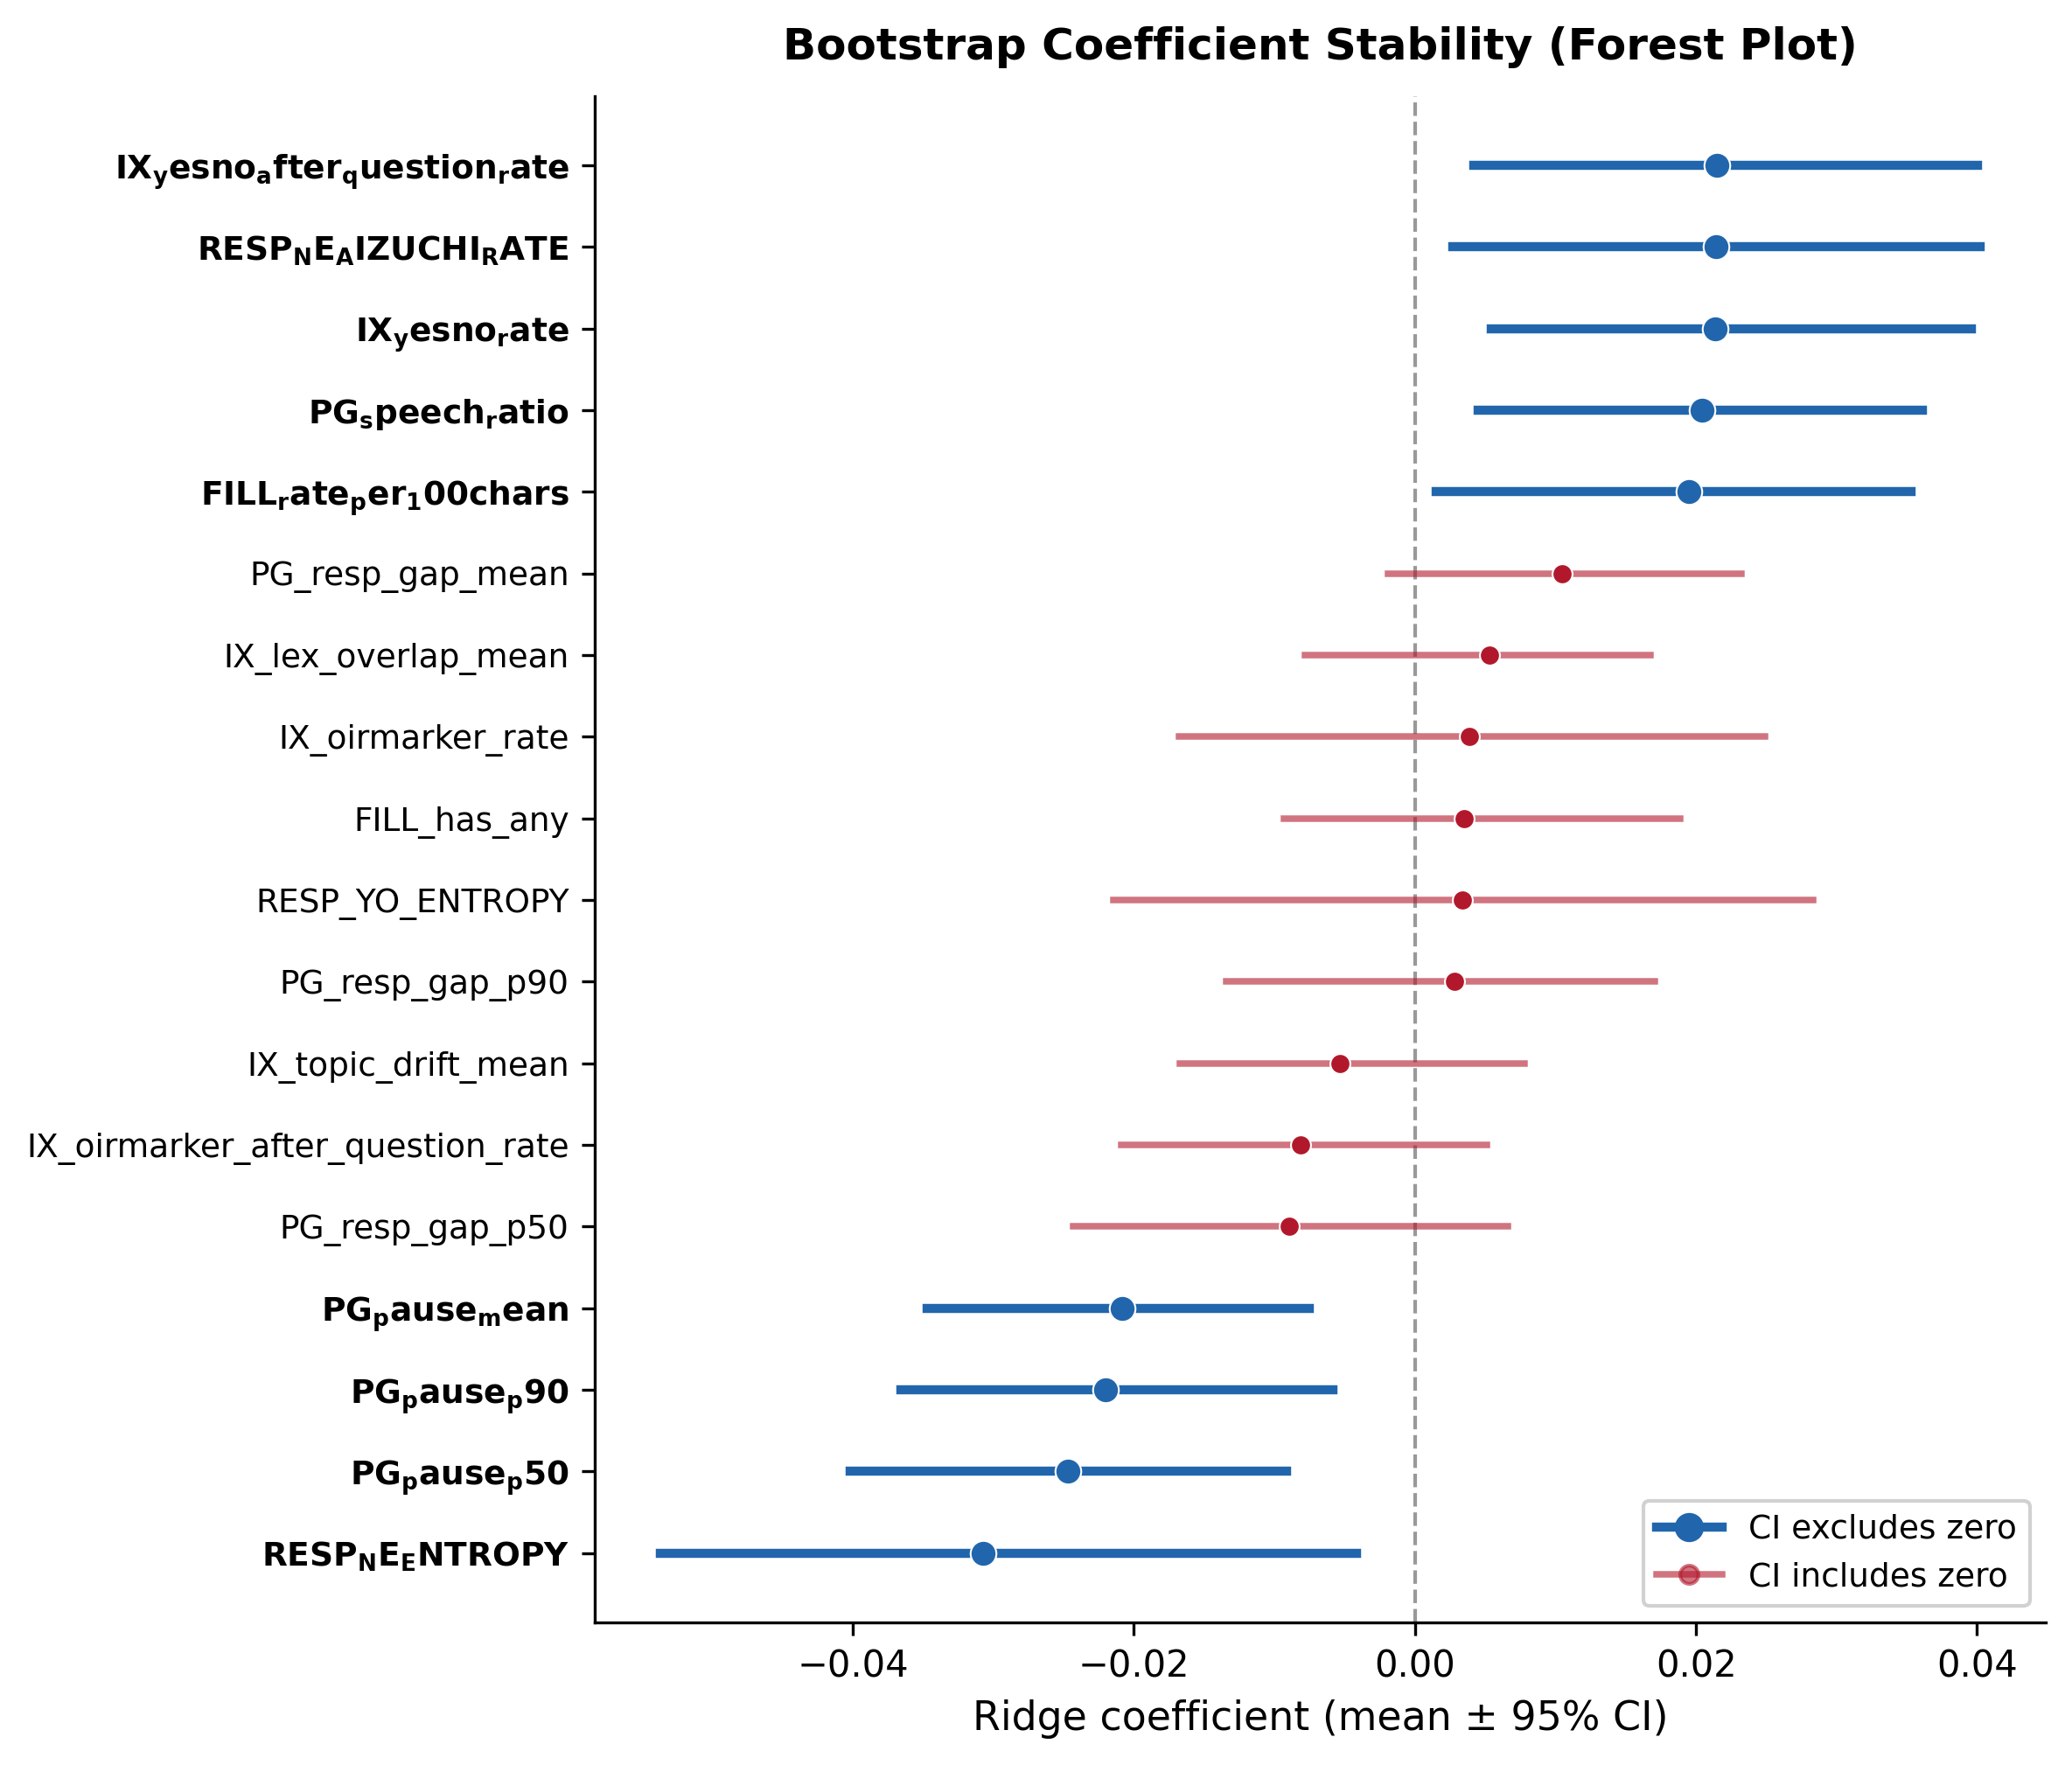
\includegraphics[width=0.9\linewidth]{fig_bootstrap_variance.png}
\caption{各特徴量の平均回帰係数$\pm$95\%CI．
破線はゼロを示す．}
\label{fig:bootstrap_variance}
\end{figure}

置換検定ならびにBootstrap法の両方で有意・安定と判定された特徴量は以下の7個である:
PG\_speech\_ratio（正の寄与），PG\_pause\_mean（負の寄与），PG\_pause\_p50（負の
寄与），PG\_pause\_p90（負の寄与），IX\_yesno\_rate（正の寄与），
IX\_yesno\_after\_question\_rate（正の寄与），RESP\_NE\_ENTROPY（負の寄与）．こ
れらの特徴量は古典的特徴量と新規特徴量の両群にまたがった．

% [NOTE] 以下のようなないようは考察に記載．結果は，基本的に事実を淡々と述べる
% > これらの共通特徴量は，Cの予測に対して最も信頼性の高い寄与特徴量として同定される．
% > これは，3.4.3節の3段階Ridge回帰比較で示された新規特徴量の付加価値と整合し，既存研究ベースの指標と新規提案の指標が相補的にCの予測に寄与していることを示す．


%% ============================================================
%%  4. Discussion
%% ============================================================
\section{考察}

\subsection{主要な知見の要約}

本研究は，日本語日常会話から相互行為の諸側面を定量化する19の特徴量を
4カテゴリ（PG: タイミング，FILL: フィラー，IX: 連鎖組織，RESP: 応答型）に
体系化し，その妥当性を2段階で検証した．
第1段階では特徴量の分布特性と相関構造を記述し，
第2段階では外部指標（話者の性別・年齢，および4つのLLMが推定した
仮想Big5スコア）との関連を検証した．
主要な知見は，会話の相互行為特徴量がConscientiousness（C）のLLMスコアを
モデル横断で最も頑健に予測することである．
この予測は，モデル全体の置換検定，個別回帰係数の置換検定，
Bootstrap安定性分析で一貫して支持され，性別・年齢を統制しても維持された．
以下では，この主要知見の解釈，特徴量の記述的性質と外部妥当性，
方法論的貢献，および限界を順に論じる．

\subsection{相互行為特徴量とBig5の関連}

本研究の主要な知見は，会話の相互行為特徴量がCのLLMスコアを
モデル横断で最も頑健に予測することである．
仮想Big5における予測精度（$r$）ではAgreeableness（A，$r = 0.449$）が
Cをわずかに上回るが，Aはモデル間一致度が低く（$\bar{r} = 0.435$），
個別モデルレベルでの有意性にばらつきがある．
これに対しCはモデル間一致度が最も高く（$\bar{r} = 0.699$），
4モデル中3モデルで有意であり，モデル横断での頑健性において最も優れている．

Permutation回帰係数検定（3.4.4節）とBootstrap分散分析（3.4.5節）の
両方で有意かつ安定と判定された共通の7特徴量——
PG\_speech\_ratio（発話率，正の寄与），
PG\_pause\_mean / PG\_pause\_p50 / PG\_pause\_p90（沈黙系3指標，負の寄与），
IX\_yesno\_rate / IX\_yesno\_after\_question\_rate（YES/NO応答率，正の寄与），
RESP\_NE\_ENTROPY（「ね」直後応答多様性，負の寄与）——が
Cの主要な関連因子として同定された．
発話率の高さと沈黙の短さは会話への積極的な参加を，
YES/NO応答率の高さは質問への明確な応答傾向を反映し，
いずれもCの高い話者に想定される丁寧で関与的な対話行動と整合する．
RESP\_NE\_ENTROPYの負の寄与は，「ね」で終わる発話への応答が
定型的（低エントロピー）であることを意味し，共感的応答の安定性として解釈できる．

これらの知見は，2種類の検定を組み合わせることで得られる．
モデル全体の置換検定（3.4.1節）がCの予測可能性そのものを示すのに対し，
個別回帰係数の置換検定はどの特徴量が予測に有意に寄与するかを同定し，
Bootstrap分散分析はその寄与のリサンプリングに対する安定性を評価する．
Permutationで有意な7特徴量はいずれもBootstrapの95\%CIがゼロを除外しており，
統計的有意性と安定性を兼ね備えた信頼性の高い寄与因子と解釈できる．
加えてBootstrapでは，FILL\_rate\_per\_100chars（100文字あたりフィラー率）と
RESP\_NE\_AIZUCHI\_RATE（「ね」直後相槌率）の2特徴量も安定と判定され，
Permutationでは有意水準に達しなかったものの注目に値する．

新規特徴量群（IX系・RESP系）の増分的な寄与は，
人口統計変数を基準に古典的特徴量・新規特徴量を段階的に追加する
3段階Ridge回帰比較（3.4.3節，表\ref{tab:three_stage}）で検討した．
人口統計のみのStage 1から古典的特徴量を加えたStage 2では
全5次元で$R^2_{\text{oof}}$が向上し（最大はE: $\Delta R^2 = +0.115$，
次いでO: $+0.107$），発話タイミング・フィラー使用が人口統計では
捉えきれない個人差を反映することが示された．
新規特徴量を加えたStage 3では3次元（O・C・N）で$R^2$が上昇しRMSEが低下したが，
paired bootstrap検定で名目的に有意な増分はNのみ（$\Delta R^2 = +0.069$,
$p_{\text{boot}} = 0.044$）であり，これもWilcoxon検定では有意でなかった（$p = 0.19$）．
他の4次元は有意でなく（$p_{\text{boot}} = 0.10$--$0.72$），
統計的に有意な悪化も認められなかった．
したがって新規特徴量はモデル全体の増分妥当性としては頑健な改善を示さず，
その実質的な寄与は個別特徴量の係数レベル（3.4.4節）で評価するのが適切である．
この段階的枠組みは，既存研究との比較可能性を担保するClassical群と，
会話分析の理論的知見を定量化するNovel群という2群構成を，
予測妥当性の観点から相補的に検討するものである．

\subsection{交絡変数の統制による予測の頑健性}

% [NOTE] このセクションは結論を中心としたより簡易な記述で問題ありません．詳細はAppendixの方に記すのがよいです．ただし，Appendixに記したように，このセクションの記載が3段階リッジと重複するものであれば削除が良いですね．3段階リッジを掲載するかどうかを踏まえて判断する必要があります．

提案特徴量の多くは性別・年齢と有意に関連するため（3.3節），
特徴量とBig5の関連が人口統計を介した交絡である可能性が残る．
この点を検証するため，相互行為特徴量のみのモデル（Model A: 19変数）に
性別・年齢を追加したモデル（Model B: 21変数）と比較した
（詳細は\ref{sec:appendix_confound}参照）．
性別・年齢を統制した後もCの有意性は3モデルで維持され，
むしろ予測精度は平均$\Delta r = +0.026$と向上した
（Claude Sonnet 4: $r = 0.360 \to 0.381$;
Qwen3-235B: $0.403 \to 0.418$;
GPT-OSS-120B: $0.452 \to 0.495$）．
これは特徴量とCの関連が性別・年齢の影響を超えた独自の寄与を持つことを示す．
精度の向上は，人口統計が特徴量では捉えきれない追加的な分散を
説明していることを示唆する．
なお本分析は，変数を追加する方向は逆だが，
人口統計を基準に特徴量を追加する3段階Ridge回帰（3.4.3節）と
相補的に特徴量の妥当性を支持するものである．

\subsection{提案特徴量の記述的性質と外部妥当性}

記述統計（3.1節）から，PG系・FILL系・RESP系の多くの特徴量は
連続的な分布を示し，話者間の行動差を段階的に捉える指標として
機能することが確認された（例: RESP\_NE\_AIZUCHI\_RATE, $SD = 0.229$）．
一方，OIR関連指標（IX\_oirmarker\_rate等）は大半の話者でゼロまたは極低値を示し，
強い正の歪度を持つ．修復開始は日常会話における低頻度事象であり，
この偏りは現象の性質を反映する．
実際，OIR率はCの有意な寄与特徴量としては同定されず
（Permutation検定: $p = 0.692$，Bootstrap CIがゼロを跨ぐ），
連続的個人差というより修復開始行動の生起を検出する二値的指標として
解釈すべきである．より大規模なデータでのOIR率の寄与の再検証は今後の課題である．

相関構造（3.2節）は特徴量セットの妥当性を支持する．
同一カテゴリ内の高い相関（PG沈黙系 $r = 0.78$--$0.97$，
応答遅れ系 $r = 0.61$--$0.94$，FILL 2指標 $r = 0.85$）は
同一構成概念の異なる集約統計量として理論的に予測され，内的整合性を示す．
一方カテゴリ間の相関は同一カテゴリ内に比べ概ね低く，多くのペアで$|r| < 0.30$であったが，
発話量に関連する一部のペア（例: PG\_speech\_ratioとFILL\_has\_any，$r = 0.61$）では
中程度の相関もみられた．全体として，PG・FILL・IX・RESPの4カテゴリは
相互に大きく重複しない会話行動の側面を捉えている．
IX\_lex\_overlap\_meanとIX\_topic\_drift\_meanの完全共線性（$r = -1.00$）は
定義上の補数関係によるもので，一方のみを用いる方針とした（2.4節）．

外部指標（性別・年齢）との関連（3.3節）は特徴量の妥当性をさらに支持する．
性別ではPG系タイミング指標に顕著な差があり，
本研究では女性の発話率が高く（$U = 950$, $p < 0.0001$）沈黙が短かった．
ただし英語圏のメタ分析\cite{leaper2007}では逆方向の小さな効果（$d = -0.14$）が
報告されており，発話量の性差は対話形式・話題・関係性に依存する\cite{bortfeld2001}．
したがって本結果は日本語の自宅・少人数会話という文脈に特有のものとして
解釈すべきである．
年齢では12特徴量が有意に相関し，PG\_speech\_ratioは正（$\rho = 0.447$），
沈黙系・応答遅れ系は負の相関を示した．
これは年齢が高い話者ほど積極的かつテンポよく応答する傾向を示し，
会話経験による流暢さとして解釈できる．
FILL系は年齢と正の相関（$\rho \approx 0.4$）を示し，
加齢に伴うフィラー増加を報告する先行研究\cite{bortfeld2001,horton2010}と整合する一方，
発話率・応答速度の年齢効果は話速低下を報告する先行知見\cite{horton2010}とは
逆であり，文脈特異性を考慮する必要がある．
注目すべきは，FILL\_rate\_per\_100charsが年齢と正の相関（$\rho = 0.391$）を示すと同時に，
CのBootstrap分散分析で安定的寄与特徴量としても同定された点であり，
フィラー使用が認知的側面（発話計画コスト）と性格的側面（Cに関連する慎重な発話）の
両方を反映する多面的指標であることを示唆する．
RESP\_NE\_AIZUCHI\_RATEと年齢の正の相関（$\rho = 0.289$）も，
年齢が高い話者ほど共感的応答を示す傾向として解釈できる．

\subsection{定量化指標としての方法論的貢献と応用可能性}

本研究の主たる貢献は，日本語日常会話における相互行為特徴量の
定量化指標の提案にある．
談話からLLM/PLMで性格特性やASD関連指標を推定する先行研究は
増えているが（Hu ら\cite{hu2025}; Wright ら\cite{wright2026};
Mun ら\cite{mun2024}），これらはLLM/PLMの出力を推定値として用いるにとどまり，
相互行為を再現可能に定量化する指標の提案には至っていない．
日本語会話コーパスを対象とした体系的検証は
Nakamura ら\cite{nakamura2025}を含めてもほとんど行われていなかった．

本研究の方法論的貢献は3点である．
第一に，19の相互行為特徴量を4カテゴリに体系化し計算アルゴリズムを
明示することで（2.2節），第三者による再現が可能な指標体系を提供した．
第二に，特徴量の分布・相関構造の記述（第一段階）と外部指標を用いた
妥当性検証（第二段階）という2段階の検証設計を採用し，
これは特徴量提案研究の一般的枠組みとして他研究にも適用できる．
第三に，subject-wise splitによるリーク防止，置換検定（5,000回），
Bootstrap（500回）による係数安定性評価，
複数LLMモデル間の一致度による頑健性検証を組み合わせた包括的評価を，
日本語会話コーパスで初めて適用した．

提案特徴量セットの適用範囲はBig5との関連に限られない．
発話タイミング・フィラー使用・修復開始・応答パターンといった
相互行為の基本側面を定量化する指標体系は，
臨床的な会話評価（例: ASD関連の社会的コミュニケーション特性），
教育場面の対話分析，高齢者の認知機能スクリーニング（年齢との関連が示唆），
異文化間コミュニケーション研究などに応用可能であり，
本研究はその最初の妥当性検証と位置づけられる．

\subsection{限界と今後の課題}

本研究には複数の限界がある．
第一に，標本サイズが$N = 120$と小さく，正則化パラメータの最適化や
より複雑なモデルの適用には不十分で，一般化可能性に制約がある．
第二に，外部検証（別コーパス・別収録条件でのクロスバリデーション）が
未実施であり，CEJCの自宅・2者間会話という限定条件に特有の結果である
可能性を排除できない．
第三に，LLMによる仮想Big5スコアを外部基準として用いているが，
これが人間の性格評定とどの程度一致するかは未検証であり，
またLLMが実際に提案特徴量に着目して推定しているかの直接的検証も
残されている．
第四に，Cに加えA/E/N/Oの一部でも有意な結果が得られており（表\ref{tab:perm_all}），
Cに寄与する特徴量が他次元にも影響する一般因子（general factor）の混入を
考慮する必要がある．
第五に，交絡統制はRidgeに統制変数を追加する方法であり，
非線形な交絡や未測定変数による残余交絡（residual confounding）を
完全には除去できない．属性分析も性別・年齢に限られ，
出身地域（方言）・職業等の社会的属性との関連は未検討である．
第六に，$N = 120$レコードは74名の話者に由来し，
25名が複数会話に参加するため重複話者由来のレコードが71件（59.2\%）に及ぶ（2.1節）．
交差検証ではGroupKFold（cejc\_person\_id単位）により直接的なリークは防止したが，
相関分析やBootstrap分析では同一話者の複数レコードを独立観測として扱っており，
レコード間の非独立性が標準誤差を過小推定するバイアスを生じうる．
同一話者が異なる会話で類似した特徴量を示すか（話者内特徴量の安定性，ICC）の
検証は今後の課題であり，提案特徴量が話者固有の安定特性か文脈依存の
状態的指標かを明らかにする上でも重要である．

%% ============================================================
%%  5. Conclusion
%% ============================================================
\section{結論}

本研究は，日本語日常会話コーパス（CEJC）の自宅・2者間会話から選定した$N = 120$レコードから抽出した
19の相互行為特徴量を用いて，4つのLLMモデルが推定したBig5スコアを
Ridge回帰で予測する枠組みを提案し，以下の知見を得た．

第一に，Conscientiousness（C）は4モデル中3モデルで有意な予測精度を示し
（$r = 0.360$--$0.452$, $p < 0.004$），特定のLLMモデルに依存しない頑健な知見であった．
仮想Big5（4モデルitem-level平均）を用いた分析では，
Eを除く4次元（O, C, A, N）で有意な関連が認められた．
Agreeableness（A）が$r = 0.449$と最高の予測精度を示したが，
モデル間一致度は$\bar{r} = 0.435$と低くモデル依存性が大きい．
一方，Cは$r = 0.432$（$p = 0.0006$）であり，
モデル横断での頑健性において最も優れていた．
第二に，Cのモデル間一致度は$\bar{r} = 0.699$と5次元中最も高く，
LLMモデルがCについて安定したスコアを付与していることが確認された．
第三に，Permutation回帰係数検定およびBootstrap分散ベース安定性分析により，
PG\_speech\_ratio（発話率），沈黙系3指標（PG\_pause\_mean / p50 / p90），
YES/NO応答率（IX\_yesno\_rate / IX\_yesno\_after\_question\_rate），
RESP\_NE\_ENTROPY（「ね」直後応答多様性）が
Cの主要な予測因子として同定された（Permutation有意かつBootstrap CIがゼロを除外する7共通特徴量）．
第四に，3段階Ridge回帰比較（人口統計のみ→古典的特徴量追加→新規特徴量追加）では，
新規提案特徴量の追加は大部分の次元で予測を劣化させず，
予測値のキャリブレーションをわずかに改善したが，
その増分妥当性は本標本（$N = 120$）ではpaired bootstrap検定で統計的に有意でなかった．
新規特徴量の実質的な寄与は，モデル全体の増分ではなく個別特徴量の係数レベル（第三の知見）で担保される．

本研究は，「性格推定」ではなく「会話の相互行為の再現可能な計測」として位置づけられ，
日本語会話コーパスにおける初の体系的検証として，
今後の研究の基盤となることが期待される．


\clearpage


%% ============================================================
%%  Appendix
%% ============================================================
\appendix


\section{会話データ}
\label{sec:supp_dataset}
% [6/22 福原] 本文2.1の詳細(選定基準の根拠・メタ紐付け・話者重複)を本節へ移送．査読者が随時参照可能（ADR-0004）．
% [NOTE] 「話者の重複と性別内訳」は本文との重複が多かったため，すべて本文に移動しました．

\subsection{選定基準}
相互行為特徴量の多くは発話ペアや特定の応答文脈における比率として定義されるため，
計算自体は会話量によらず可能である（分母がゼロとなる場合を除く）．ただし，観測数
が少ないと比率推定の標本変動が大きくなり，個々人の相互行為傾向を安定して反映しな
くなる．そこで，個々人の相互行為を反映できるような十分な会話量を担保するために，
以下の性質を有するデータのみを選定した．

\begin{enumerate}
  \item 発話ペア数 $\geq 80$: 話者交替時の前発話と応答のペア数が80以上であること．
IX系（修復開始率，YES/NO応答率等）およびRESP系（終助詞直後応答パターン）の特徴量
は隣接ペアに基づく比率であり，ペア数が少ないと少数観測に基づく推定となって標本変
動が大きくなる．
  \item テキスト文字数 $\geq 2{,}000$: 当該話者の全発話を連結したテキストの文字数
（空白除去後）が2,000文字以上であること．FILL系（フィラー率）などの文字数正規化指
標が十分なテキスト量に基づくようにするために設けた．
  \item 質問直後ペア数 $\geq 10$: 前発話が質問である応答ペアが10以上であること．
IX\_oirmarker\_after\_question\_rateおよびIX\_yesno\_after\_question\_rateは質問
直後の応答に限定した指標であり，分母が極端に少ないと比率推定の標本変動が大きくな
る．
\end{enumerate}


\subsection{CEJCメタ情報の紐付け}
分析の基本単位は conversation\_id $\times$ cejc\_person\_id のペアである．
話者の属性情報（性別，年齢帯等）はCEJCのメタデータファイル（話者.csv）に
cejc\_person\_idをキーとして格納され，各話者の参加会話は
話者会話対応表（話者会話対応表.csv）に conversation\_id $\times$ cejc\_person\_id
の組み合わせで記録されている．これらを統合し，$N = 120$レコード全件で
話者属性の紐付けに成功した（\ref{sec:result_metadata}節の属性情報との関連分析に使用）．

\section{LLMによる仮想Big5スコア推定}
\label{sec:big5score}

\subsection{手続き}

LLMを用いて各話者の性格特性（Big5スコア）を推定しリッジ回帰分析における目的変数
とした．Big5の測定には，自己報告式質問紙尺度であるInternational Personality Item
Pool（IPIP-NEO-120，日本語版120項目，5件法）を使用した．LLMモデルは，会話テキス
トを参照しながらIPIP-NEO-120の各項目に回答した．項目ごとの回答の算術平均
によって5つの性格次元（Openness: O, Conscientiousness: C, Extraversion: E,
Agreeableness: A, Neuroticism: N）のスコアを算出した．話者の性格推定が特定のLLM
モデルに依存しないように4つのLLMモデルから推定されたスコアを平均して用いた．使用
した4モデルは以下の通りである．

% [NOTE] 以下の記載は(1), (3)は重複していますし(2)は読者に共有する情報ではないと感じます．そのため，修正いたしました．
% > これにより，(1) 特定のLLM教師に依存しない安定した推定値が得られること，(2) 個別教師ごとの結果一覧による混乱を回避し，単一の推定値に基づく明快な報告が可能となること，(3) 教師間のばらつきが平均化により安定化されることが期待された．

\begin{itemize}
  \item Anthropic Claude Sonnet 4（プロプライエタリ）
  \item Alibaba Qwen3-235B（オープンウェイト）
  \item DeepSeek DeepSeek-V3（オープンウェイト）
  \item OpenAI GPT-OSS-120B（オープンウェイト）
\end{itemize}

各モデルは「ベンダー名＋公式モデル識別子」で表記し，パラメータ数は非公開モデルを
含むため併記せず，公開区分（プロプライエタリ／オープンウェイト）を付す
\cite{wright2026}．

各モデルはAWS Bedrock経由で推論を実行し，同一の会話$\times$話者ペアに対して独立
にスコアを付与した．なお，複数のLLMによるゼロショット採点の平均が自
己報告のBig5と収束的妥当性を示すことはWright ら\cite{wright2026}が報告している．

% [NOTE] 以下の記載は意義などが含まれるように聞こえるため，可能な限り短縮して記載しています．意義のような記載は極力背景や考察に書くようにします．
% > なお，複数のLLMによるゼロショット採点のアンサンブル平均が自己報告のBig5と収束的妥当性を示すことはWright ら\cite{wright2026}が報告しており，本研究の仮想教師プロトコルはこのアプローチを日本語会話コーパスに適用・拡張したものと位置づけられる．

\subsection{IPIP-NEO-120の項目例}
\label{sec:appendix_ipip}

IPIP-NEO-120は5つの性格次元（O, C, E, A, N）に対応する120項目から構成される．各
次元24項目のうち12項目が正方向，12項目が逆転項目である．以下に各次元の代表的な項
目例を示す:

\begin{itemize}
  \item Openness（O）: ``I have a vivid imagination.'' / ``I am not interested in abstract ideas.''（逆転）
  \item Conscientiousness（C）: ``I am always prepared.'' / ``I make a mess of things.''（逆転）
  \item Extraversion（E）: ``I am the life of the party.'' / ``I don't talk a lot.''（逆転）
  \item Agreeableness（A）: ``I sympathize with others' feelings.'' / ``I am not interested in other people's problems.''（逆転）
  \item Neuroticism（N）: ``I get stressed out easily.'' / ``I seldom feel blue.''（逆転）
\end{itemize}

IPIP-NEO-120の全120項目リストはIPIP公式サイト（\url{https://ipip.ori.org/newNEO_DomainsTable.htm}）から取得した．

\subsection{プロンプトテンプレート}
\label{sec:appendix_prompt}

本研究では，各LLMモデルに対して以下のプロンプトテンプレートを用いてIPIP-NEO-120
の各項目を5件法で回答させた．温度パラメータは$T = 0.0$（決定的出力），乱数シード
は$\text{seed} = 0$で固定した．

\paragraph{System prompt}

\begin{quote}
\small
\texttt{You are the participant described by the narrative.
Answer the survey item as that person.
You must output ONLY one of the allowed choices, exactly.}
\end{quote}

\paragraph{User prompt}

\begin{quote}
\small
\texttt{Below is a narrative written by a participant (the person you must respond as).}\\[4pt]
\texttt{=== NARRATIVE (participant diary / transcript) ===}\\
\texttt{\{conversation\_text\}}\\
\texttt{=== END NARRATIVE ===}\\[4pt]
\texttt{Now answer the following personality item as though you are that individual.}\\
\texttt{Output MUST be exactly one of the following choices (no extra characters, no punctuation, no explanation):}\\
\texttt{Very Inaccurate}\\
\texttt{Moderately Inaccurate}\\
\texttt{Neither Accurate Nor Inaccurate}\\
\texttt{Moderately Accurate}\\
\texttt{Very Accurate}\\[4pt]
\texttt{ITEM: \{item\_text\}}\\
\texttt{ANSWER:}
\end{quote}

ここで \texttt{\{conversation\_text\}} は当該話者の全発話を時系列順に連結したテ
キスト，\texttt{\{item\_text\}} はIPIP-NEO-120の各項目文である．項目文は英語のま
ま使用し，LLMには日本語の会話テキストと英語の項目文を同時に提示した．LLMの出力は
上記5選択肢のいずれか1つのみを期待し，Very Inaccurate $= 0$, Moderately
Inaccurate $= 1$, Neither $= 2$, Moderately Accurate $= 3$, Very Accurate $= 4$
として数値化した．逆転項目は $4 - \text{score}$ で反転処理した．各次元のスコアは
対応する24項目の平均として算出した．





\section{特徴量間相関行列}
\label{sec:supp_corr}
% [6/22 福原] 3.2のヒートマップ(図)と重複する19x19数値行列を本文から補足へ移送(ADR-0014)．宗田さんが削除指示したColumn keyは、番号列(1)-(19)の解釈に必要なため数値表とともに本補足にのみ残す．
表\ref{tab:corr_matrix}に相互行為特徴量間のPearson相関係数を示す．

\begin{table}[htbp]
\centering
\caption{相互行為特徴量間のPearson相関行列．}
\label{tab:corr_matrix}
\input{reports/paper_figs_v2/tab_corr_matrix.tex}
\end{table}





\section{コーパス基本情報との関連}
\label{sec:appendix_metadata}

図\ref{fig:metadata_gender}, \ref{fig:metadata_age}に，それぞれ相互行為特徴量と性別，年齢との関連を示す．

\begin{figure}[p]
\centering
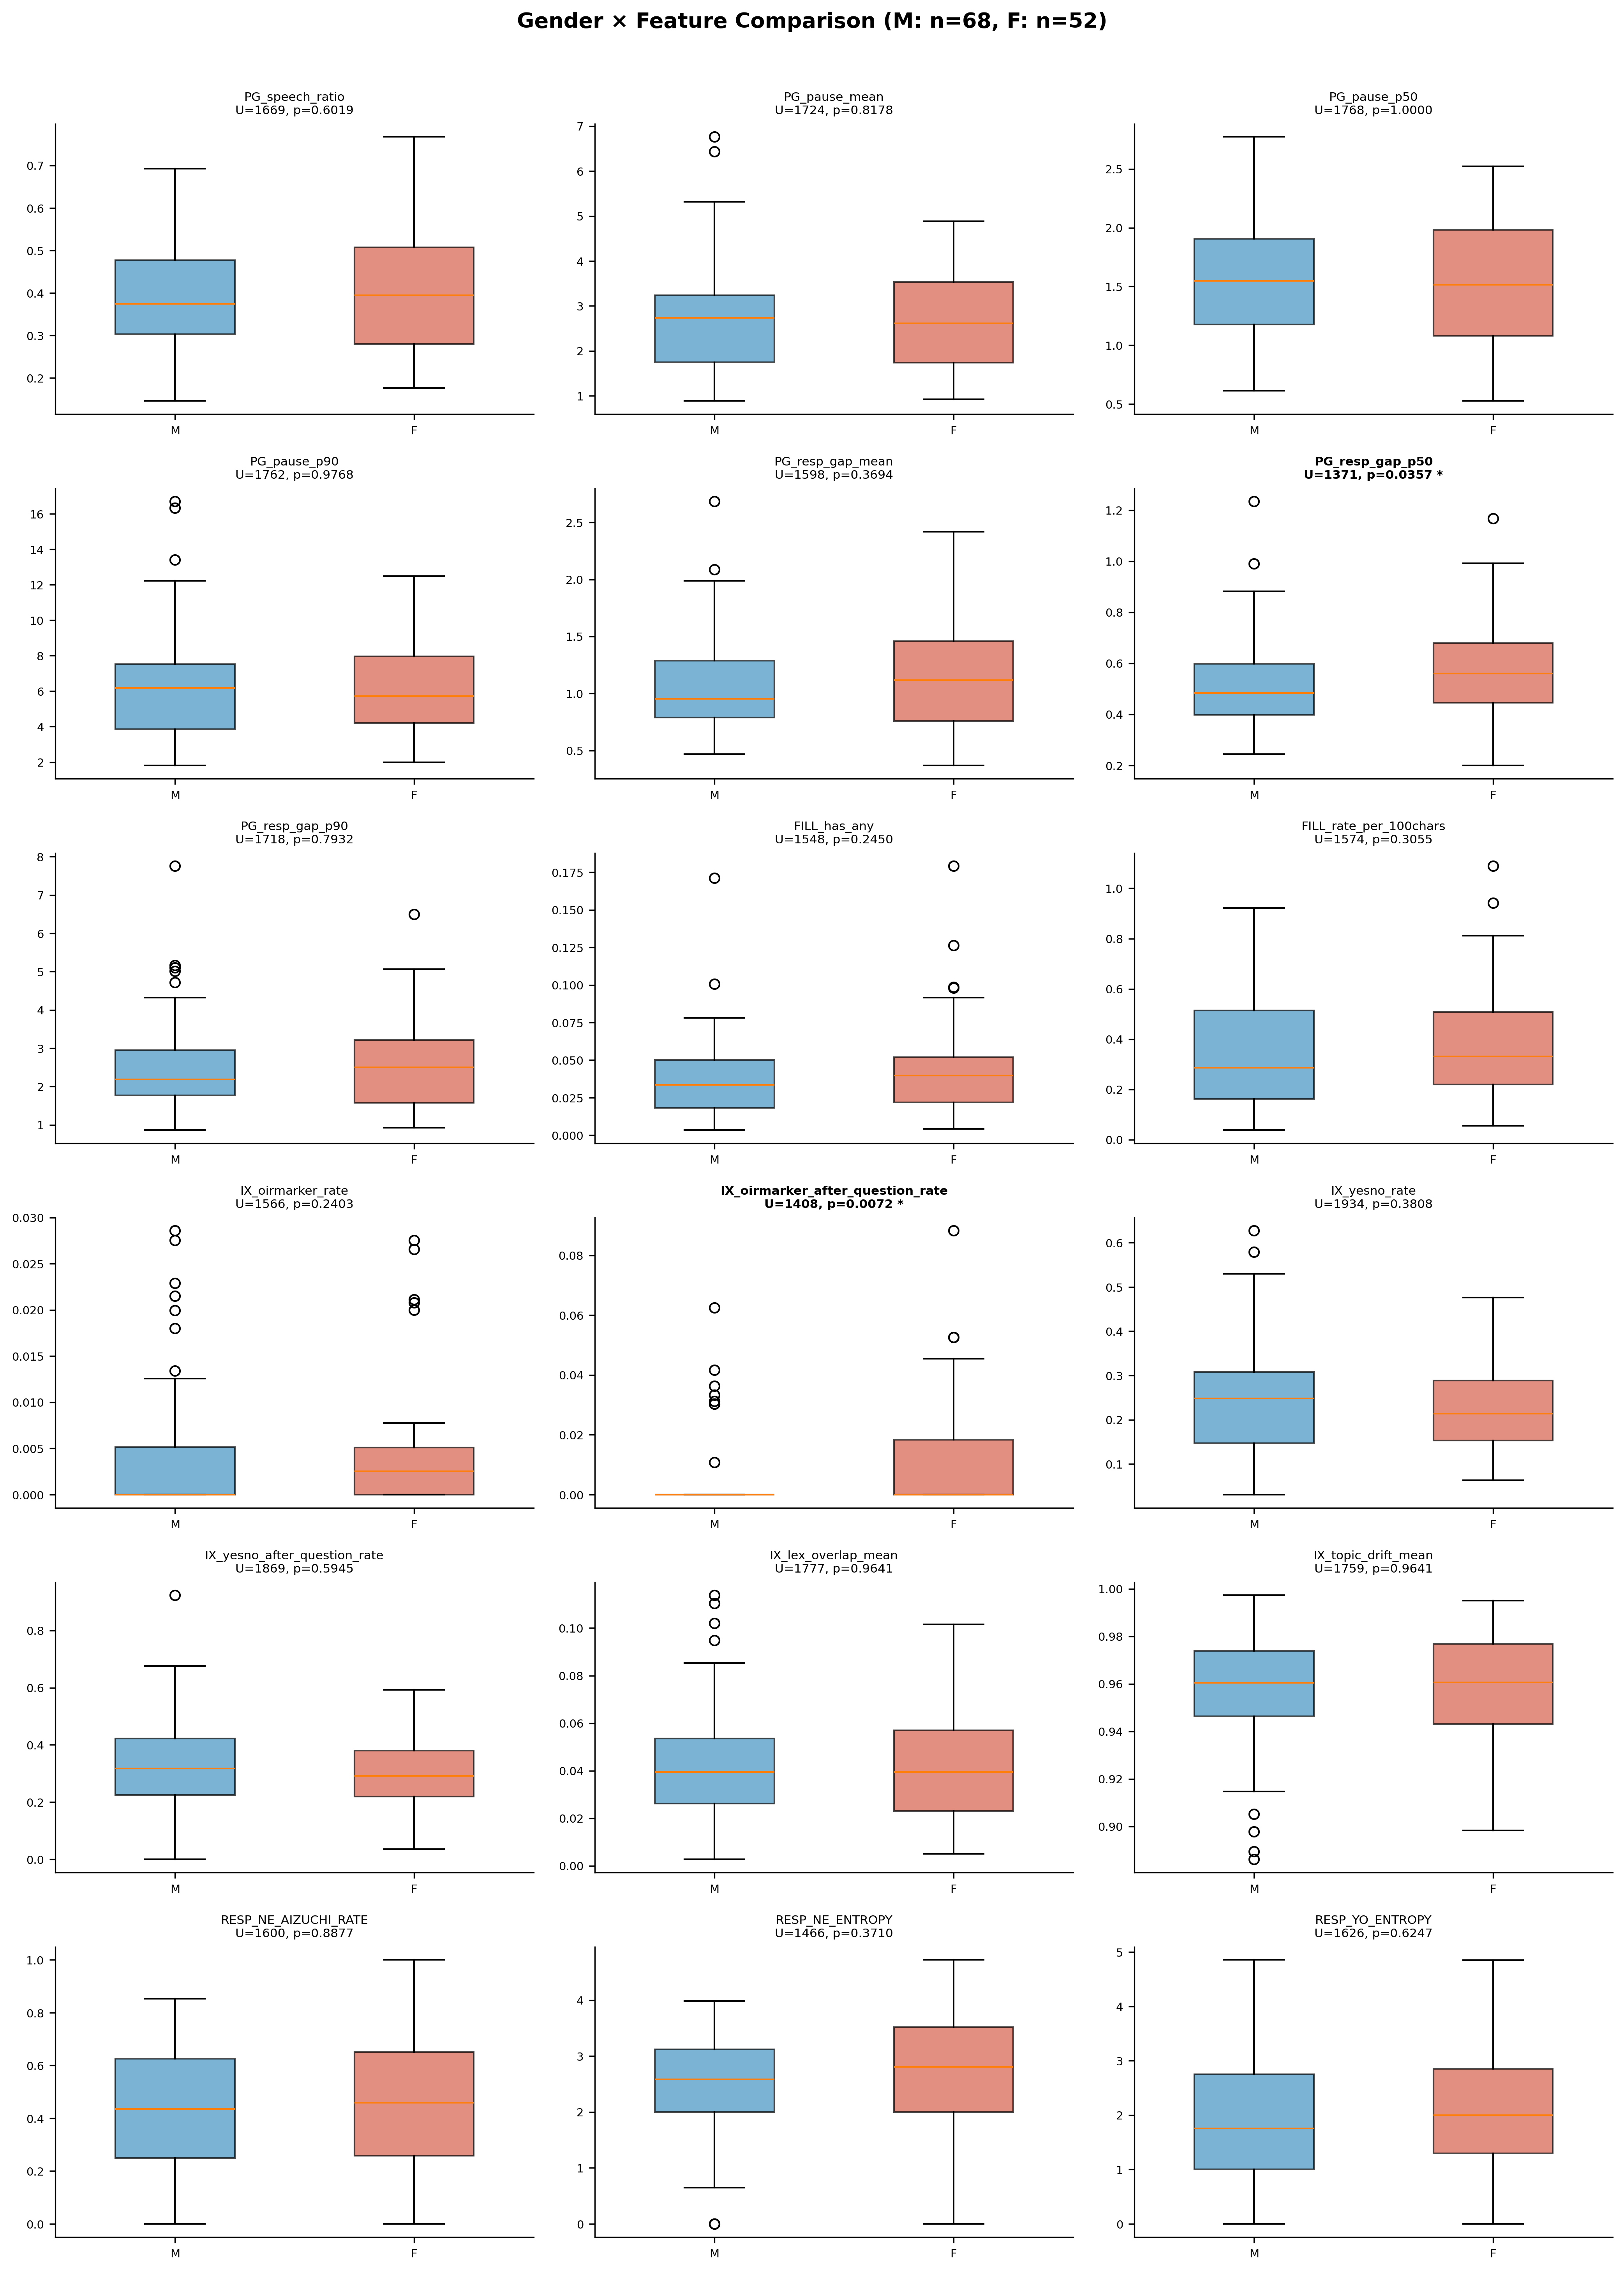
\includegraphics[width=0.95\linewidth]{fig_metadata_gender.png}
\caption{性別と特徴量の関連．
M: 男性（$n=54$），F: 女性（$n=66$）．$*$は$p < 0.05$を示す．}
\label{fig:metadata_gender}
\end{figure}

\begin{figure}[p]
\centering
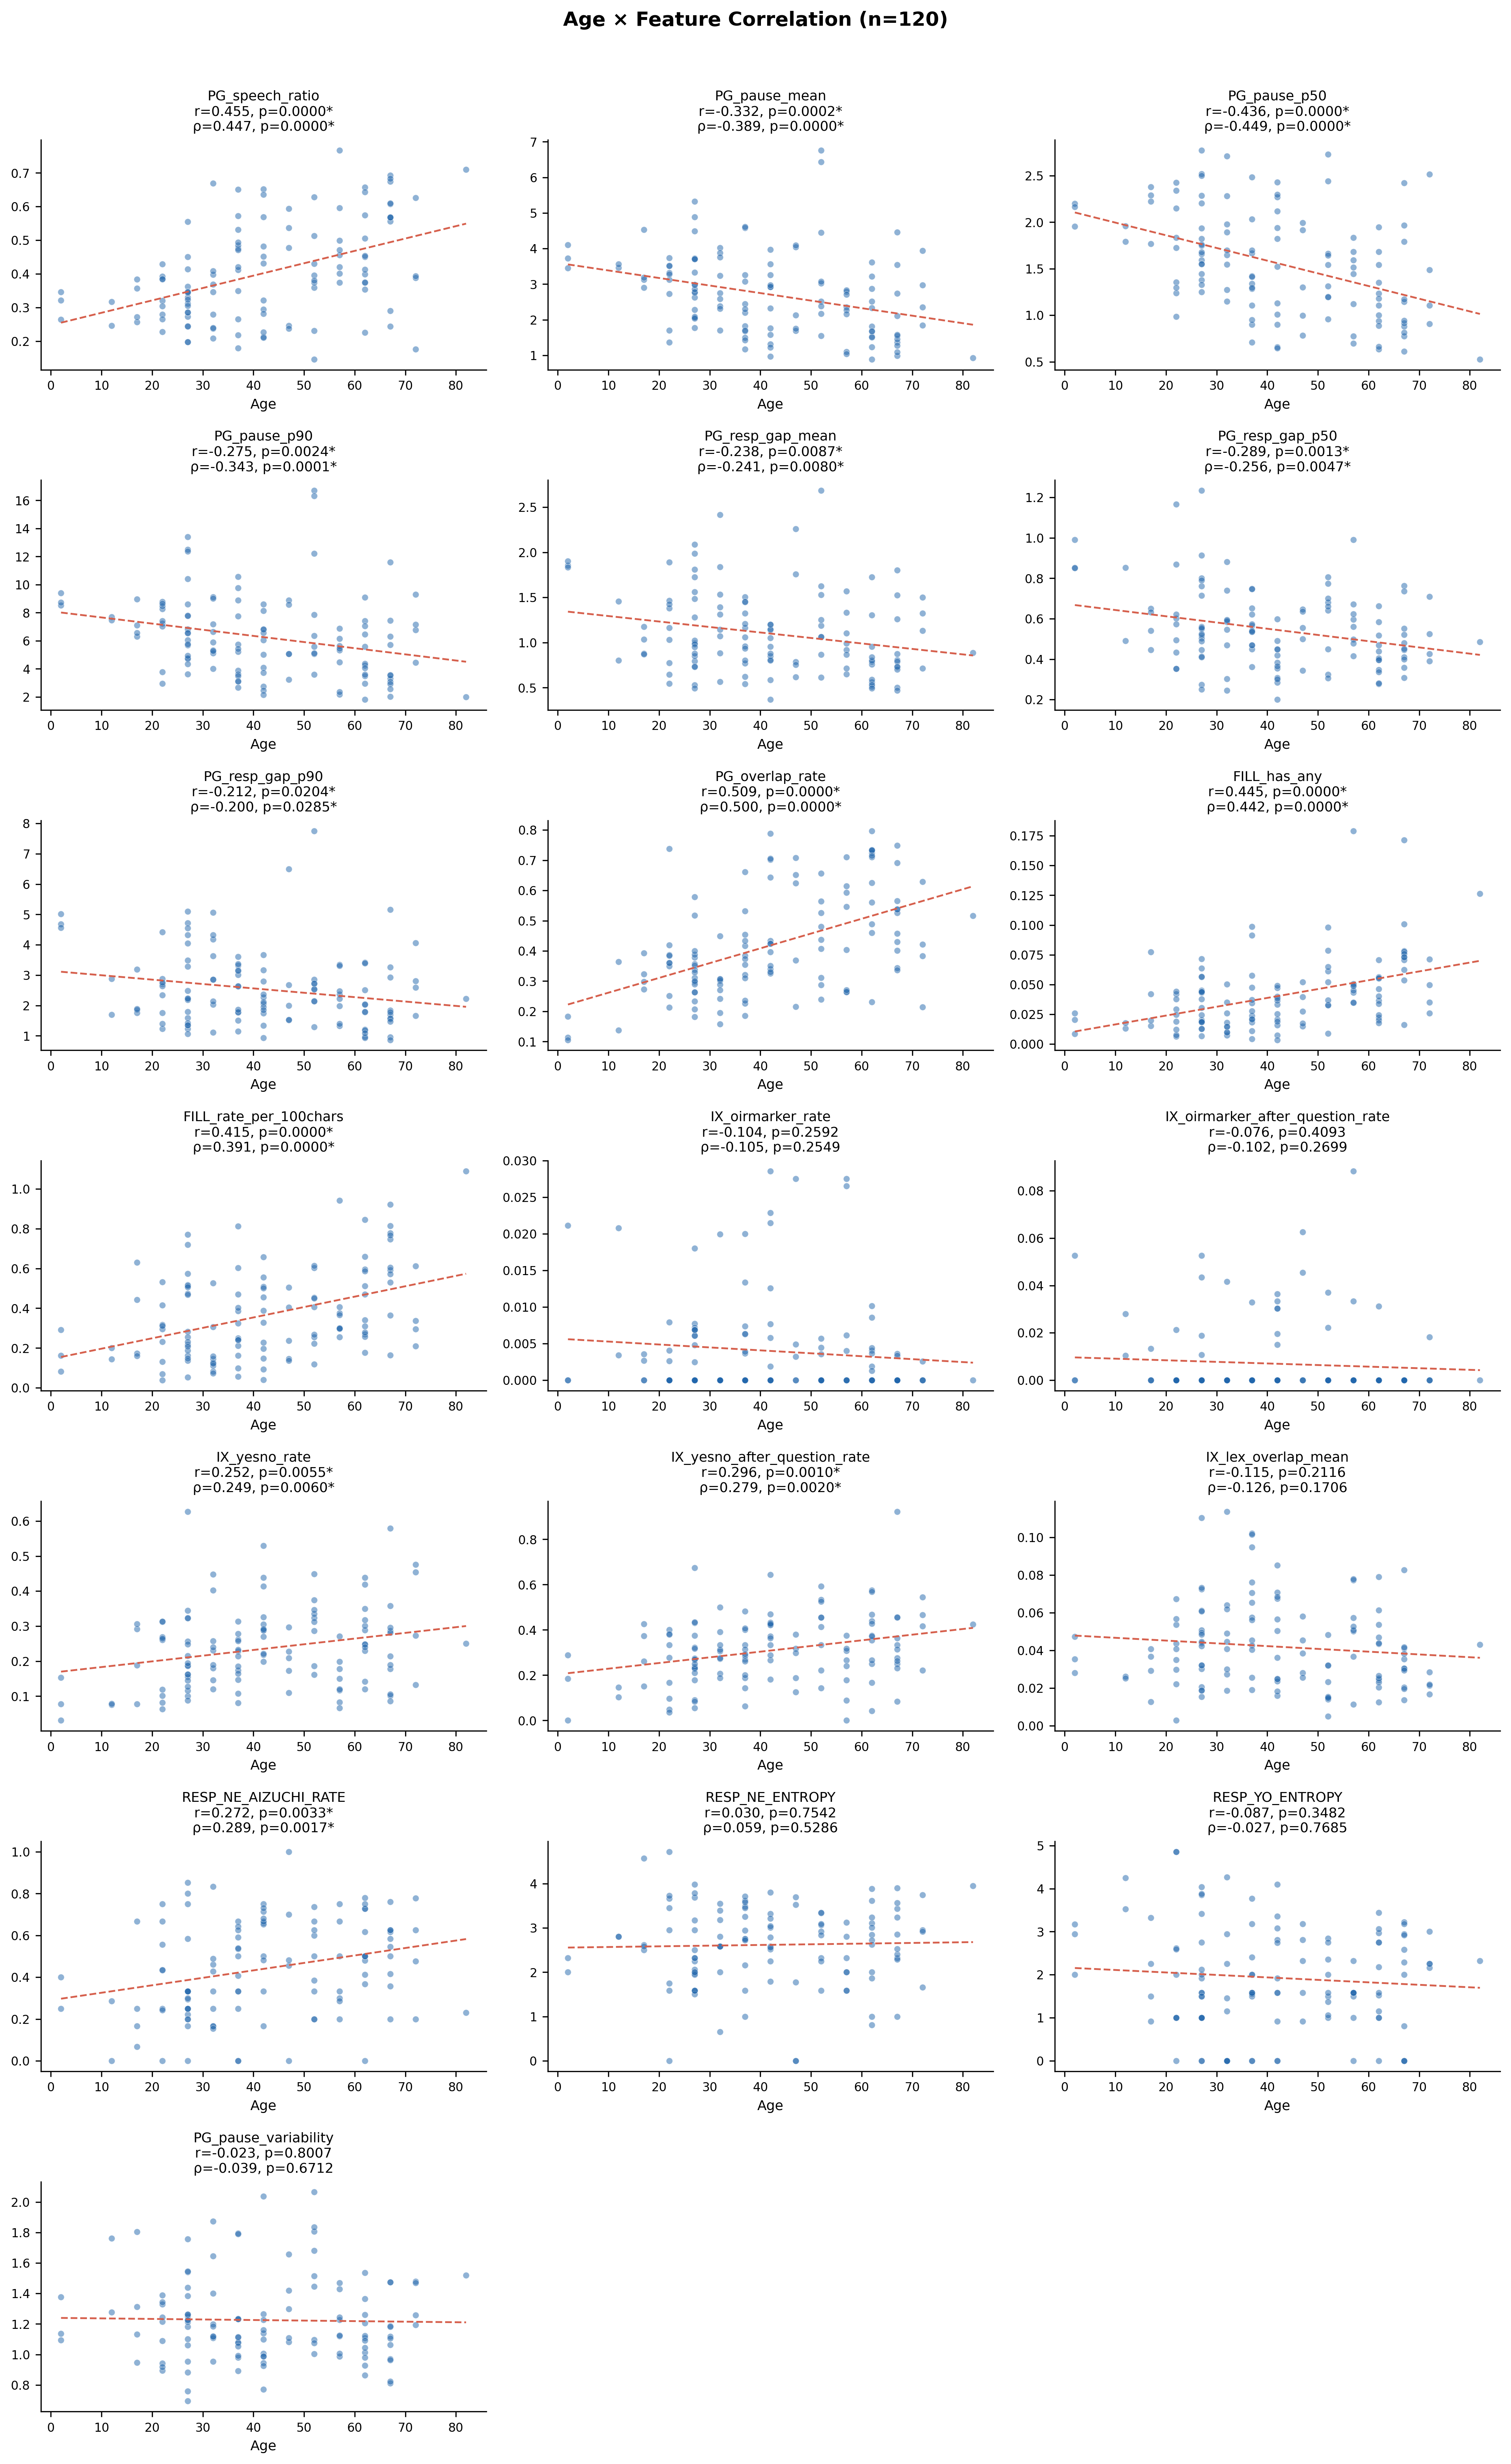
\includegraphics[width=0.90\linewidth]{fig_metadata_age.png}
\caption{年齢と特徴量の関連．
  各点は1話者を表す．$r$, $rho$は，それぞれPearson相関係数，Spearman相関係数示す．$*$は$p < 0.05$を示す．}
\label{fig:metadata_age}
\end{figure}





\section{3段階Ridge回帰比較（相関$r$版）}
\label{sec:appendix_three_stage_r}

% [山下6/22適用] 本文3.4.3の主指標をR²/RMSEへ変更したため、相関r版を透明性のため付録に保持．
% [NOTE] この相関係数の結果については本文の表に合流させるのが良いかと思います．ただ，3段階リッジを含めるかどうか決めた後に調整する方が効率良さそうなので一旦後回しとします．

本文3.4.3節では，予測寄与の評価により適した指標として
OOF-pooled $R^2$および予測誤差RMSEを主指標とした．
透明性のため，同一のCV設定（Ridge $\alpha=100$，5-fold subject-wise CV）で算出した
相関$r$に基づく集計を表\ref{tab:three_stage_r}に示す．
$r_{\text{oof}}$は全標本のOOF予測を連結して算出したPearson相関，
$r_{\text{foldmean}}$は各foldの$r$を平均した値である．
相関$r$による集計では，Novel追加（Stage 2→3）でOの増分が負（$\Delta r_{\text{oof}} = -0.017$）に転じる一方，
$R^2$・RMSEでは改善側に評価される（本文表\ref{tab:three_stage}参照）．
これは$r$が予測値の縮約に伴うキャリブレーションのずれを反映しないことに起因する．

\begin{table}[htbp]
\centering
\caption{3段階Ridge回帰比較（相関$r$版・参考）．
$r_{\text{oof}}$はOOF予測連結によるPearson相関，
$r_{\text{foldmean}}$は5-fold平均，$\Delta r_{\text{oof}}$は隣接ステージ間の増分．}
\label{tab:three_stage_r}
\begin{tabular}{llrccc}
\toprule
Trait & Stage & $n_{feat}$ & $r_{oof}$ & $r_{foldmean}$ & $\Delta r_{oof}$ \\
\midrule
O & Demographics & 2 & 0.270 & 0.336 & --- \\
 & +Classical & 12 & 0.491 & 0.512 & +0.222 \\
 & +Novel & 21 & 0.474 & 0.481 & -0.017 \\
\midrule
C & Demographics & 2 & 0.404 & 0.425 & --- \\
 & +Classical & 12 & 0.383 & 0.398 & -0.021 \\
 & +Novel & 21 & 0.443 & 0.469 & +0.060 \\
\midrule
E & Demographics & 2 & 0.004 & 0.156 & --- \\
 & +Classical & 12 & 0.262 & 0.291 & +0.258 \\
 & +Novel & 21 & 0.200 & 0.237 & -0.062 \\
\midrule
A & Demographics & 2 & 0.479 & 0.529 & --- \\
 & +Classical & 12 & 0.474 & 0.528 & -0.005 \\
 & +Novel & 21 & 0.505 & 0.538 & +0.031 \\
\midrule
N & Demographics & 2 & 0.100 & 0.186 & --- \\
 & +Classical & 12 & 0.169 & 0.235 & +0.070 \\
 & +Novel & 21 & 0.268 & 0.311 & +0.099 \\
\bottomrule
\end{tabular}

\end{table}



% [NOTE] 以下「Bootstrap安定性分析の詳細」は，内容が重複しているため削除．

% \section{Bootstrap安定性分析の詳細}
% \label{sec:appendix_bootstrap}

% 本文3.4.4--3.4.5節で報告したPermutation回帰係数検定およびBootstrap分散ベース安定性分析の
% 補足情報を以下に示す．

% \paragraph{Bootstrap分散分析の補足}
% 500回のBootstrapリサンプリングにおける各特徴量の回帰係数のSD（標準偏差）は，
% リサンプリングに対する係数推定の安定性を反映する．
% SDが小さい特徴量は，データの変動に対して安定的に寄与する特徴量と解釈される．
% 95\%CI（2.5--97.5パーセンタイル）がゼロを跨がない特徴量は，
% 係数の符号が一貫しており影響が強い特徴量として同定される．

% \paragraph{参考: Top-K inclusion rateおよび符号一致率}
% 補助的な指標として，各特徴量がBootstrap反復においてTop-K（$K = 5$，
% 回帰係数の絶対値上位5変数）に選ばれる頻度（Top-K inclusion rate）と，
% 係数の符号が観測値と一致する割合（符号一致率）も算出した．
% RESP\_NE\_ENTROPY（topk\_rate $= 0.89$），
% PG\_pause\_p50（topk\_rate $= 0.76$），
% PG\_pause\_mean（topk\_rate $= 0.72$）が上位3変数として安定的に選出された．
% 上位3変数の符号一致率（sign\_agree\_rate）はいずれも0.90以上であり，
% 係数の方向（正/負）がBootstrap反復間で一貫していることが確認された．
% なお，$K = 5$は相互行為特徴量の約26\%に相当し，
% 主要な寄与特徴量を同定するための探索的な閾値として設定した．





\section{性格特性予測の感度分析}
\label{sec:appendix_sensitivity}

性格特性予測に関する頑健性を検証するため，以下の感度分析を実施した．

\subsection{正則化パラメータ$\alpha$}
Ridge回帰の正則化パラメータ$\alpha$を$\{10, 50, 100, 200, 500\}$の範囲で変化させ，
Cの予測精度（$r_{\text{obs}}$）と置換検定（5,000回）による$p$値の変動を確認した
（表\ref{tab:sensitivity_alpha}）．特徴量集合は本文と同一の19変数に固定し，$\alpha$
のみを変化させた（$\alpha = 100$は本文で採用した主モデルに一致する）．$r_{\text{obs}}$
は検討した全範囲で$0.42$--$0.43$の狭い範囲に収まり，$p$値はいずれも$0.001$未満で
あった．すなわち，Cの有意性は$\alpha$の選択に対して頑健である．

\begin{table}[htbp]
\centering
\caption{正則化パラメータ$\alpha$に対する感度（Big5次元C，4モデル平均，
5-fold CV，置換検定5,000回）．$^{\dagger}$は本文で採用した$\alpha = 100$を表す．
$\alpha = 100$の$r_{\text{obs}} = 0.4315$は本文の3桁表記$0.432$に対応する．}
\label{tab:sensitivity_alpha}
\input{reports/paper_figs_v2/tab_sensitivity_alpha.tex}
\end{table}

\subsection{交絡変数（性別・年齢）の統制}
\label{sec:appendix_confound}

本文の考察で言及した交絡変数（性別・年齢）の統制分析の詳細を以下に示す．相互行為特徴量のみのモデル（Model A: 19説明変数）と，相互行為特徴量に性別（ダミー変数: M=0, F=1）および年齢を追加したモデル（Model B: 21説明変数）の2条件でRidge回帰（$\alpha = 100$，5-fold GroupKFold CV）+ 置換検定（1,000回）を実行した．

交絡変数を統制した後もCの有意性が維持されるかどうかを検証した．性別・年齢を説明変数に追加した場合の予測精度の変化（$\Delta r$）と$p$値の変化を報告する．Cについては，交絡統制前に有意であった3モデル（Claude Sonnet 4, Qwen3-235B, GPT-OSS-120B）はいずれも統制後も有意性を維持し，平均$\Delta r = +0.026$と精度が向上した．DeepSeek-V3は統制前後ともに非有意であった．

この結果は，Cと相互行為特徴量の関連が性別・年齢の交絡によるものではなく，
特徴量が独自の予測情報を持つことを示す．

この交絡統制分析は，本文の3段階Ridge回帰（表\ref{tab:three_stage}）とは目的・変数投入の方向・評価指標が異なる．3段階Ridgeは人口統計（性別・年齢）を基準（Stage 1）とし，そこにClassical・Novel特徴量を段階的に追加して特徴量の増分予測価値をOOF連結の$R^2$・RMSEとpaired bootstrapで評価する．一方，本節の交絡統制は特徴量（19変数）を基準とし，そこに性別・年齢を追加して特徴量とCの関連が人口統計の交絡で説明されないことを予測精度$r$と置換検定で確認する．すなわち両者は変数を追加する方向が逆であり，前者は特徴量の追加価値，後者は特徴量の交絡頑健性という相補的な問いに答える．


\section{LLMモデル間の差異}
\label{sec:appendix_llm}

\subsection{仮想Big5スコアの基本統計量}
\label{sec:appendix_score_stats}

表\ref{tab:score_stats}に，4つのLLMモデルが推定した各Big5の次元の基本統計量を示す．

% [NOTE] 以下のような分野において当然とされる情報は不要です．
% > これらの統計量は，$N = 120$レコードに対する推定値の分布特性を要約するものである．

\begin{table}[htbp]
\centering
\caption{推定Big5スコアの基本統計量（$N = 120$）．}
\label{tab:score_stats}
\begin{tabular}{llrrrr}
\toprule
次元 & LLM & 平均 & SD & 最小値 & 最大値 \\
\midrule
O & Claude Sonnet 4       & 2.3 & 0.3 & 1 & 3 \\
O & Qwen3-235B    & 2.5 & 0.2 & 2 & 3 \\
O & DeepSeek-V3   & 2.5 & 0.6 & 1 & 4 \\
O & GPT-OSS-120B  & 2.0 & 0.5 & 1 & 3 \\
\midrule
C & Claude Sonnet 4       & 2.1 & 0.4 & 1 & 3 \\
C & Qwen3-235B    & 2.5 & 0.3 & 2 & 4 \\
C & DeepSeek-V3   & 2.3 & 0.5 & 1 & 3 \\
C & GPT-OSS-120B  & 2.3 & 0.7 & 1 & 4 \\
\midrule
E & Claude Sonnet 4       & 2.2 & 0.4 & 1 & 3 \\
E & Qwen3-235B    & 1.7 & 0.4 & 1 & 3 \\
E & DeepSeek-V3   & 1.7 & 0.4 & 1 & 3 \\
E & GPT-OSS-120B  & 1.8 & 0.5 & 1 & 3 \\
\midrule
A & Claude Sonnet 4       & 2.8 & 0.3 & 2 & 3 \\
A & Qwen3-235B    & 2.9 & 0.2 & 2 & 4 \\
A & DeepSeek-V3   & 3.0 & 0.3 & 3 & 4 \\
A & GPT-OSS-120B  & 2.7 & 0.5 & 1 & 4 \\
\midrule
N & Claude Sonnet 4       & 2.0 & 0.4 & 1 & 4 \\
N & Qwen3-235B    & 1.7 & 0.3 & 1 & 3 \\
N & DeepSeek-V3   & 1.2 & 0.5 & 0 & 3 \\
N & GPT-OSS-120B  & 1.9 & 0.5 & 1 & 3 \\
\bottomrule
\end{tabular}
\end{table}


\subsection{仮想Big5スコアのモデル間一致度}
\label{sec:appendix_teacher_agreement}
% [山下6/22適用] 本文3.4.6節を本付録へ移設．定義・ヒートマップ・相関行列を統合．

本研究の知見が使用するLLMモデルの影響を受けるかどうか検討するために，まず4つの
LLMモデル間のBig5スコアの一致度を分析した．具体的には，120件のレコードそれぞれに
対して，4つのLLMモデルがIPIP-NEO-120に基づいて算出したBig5スコアを取得し，モデル
ペアごとにスコア間のPearson相関係数を，モデル間一致度として算出した．これにより，
各Big5次元について$4 \times 4$のモデル間相関行列が得られる．モデル間一致度が高い
次元では，LLMモデルの選択に依存しない安定した推定値が得られるため，その次元にお
けるモデルごとの回帰分析結果の頑健性が高いと解釈できる．


図\ref{fig:teacher_corr_matrix_appendix}に，性格次元それぞれのモデル間一致度を示
す．各パネルは，一つのBig5次元に対応する．モデル間一致度は，性格次元によって異な
ることが読み取れる．例えば，Conscientiousnessは全モデルペアで$r > 0.6$と高い一致
を示す一方，Aではモデルペアによって$r$の値に大きなばらつきが認められる．性格次元
ごとの差異がわかりやすくなるように，モデル間で平均を取り，性格次元ごとのモデル間
一致度を求めた（図\ref{fig:teacher_heatmap}）．この値は，Conscientiousnessにおい
て$\bar{r} = 0.699$であり5次元中最も高く，Agreeablenessにおいて$\bar{r} = 0.435$
と最も低かった．

\begin{figure}[p]
\centering
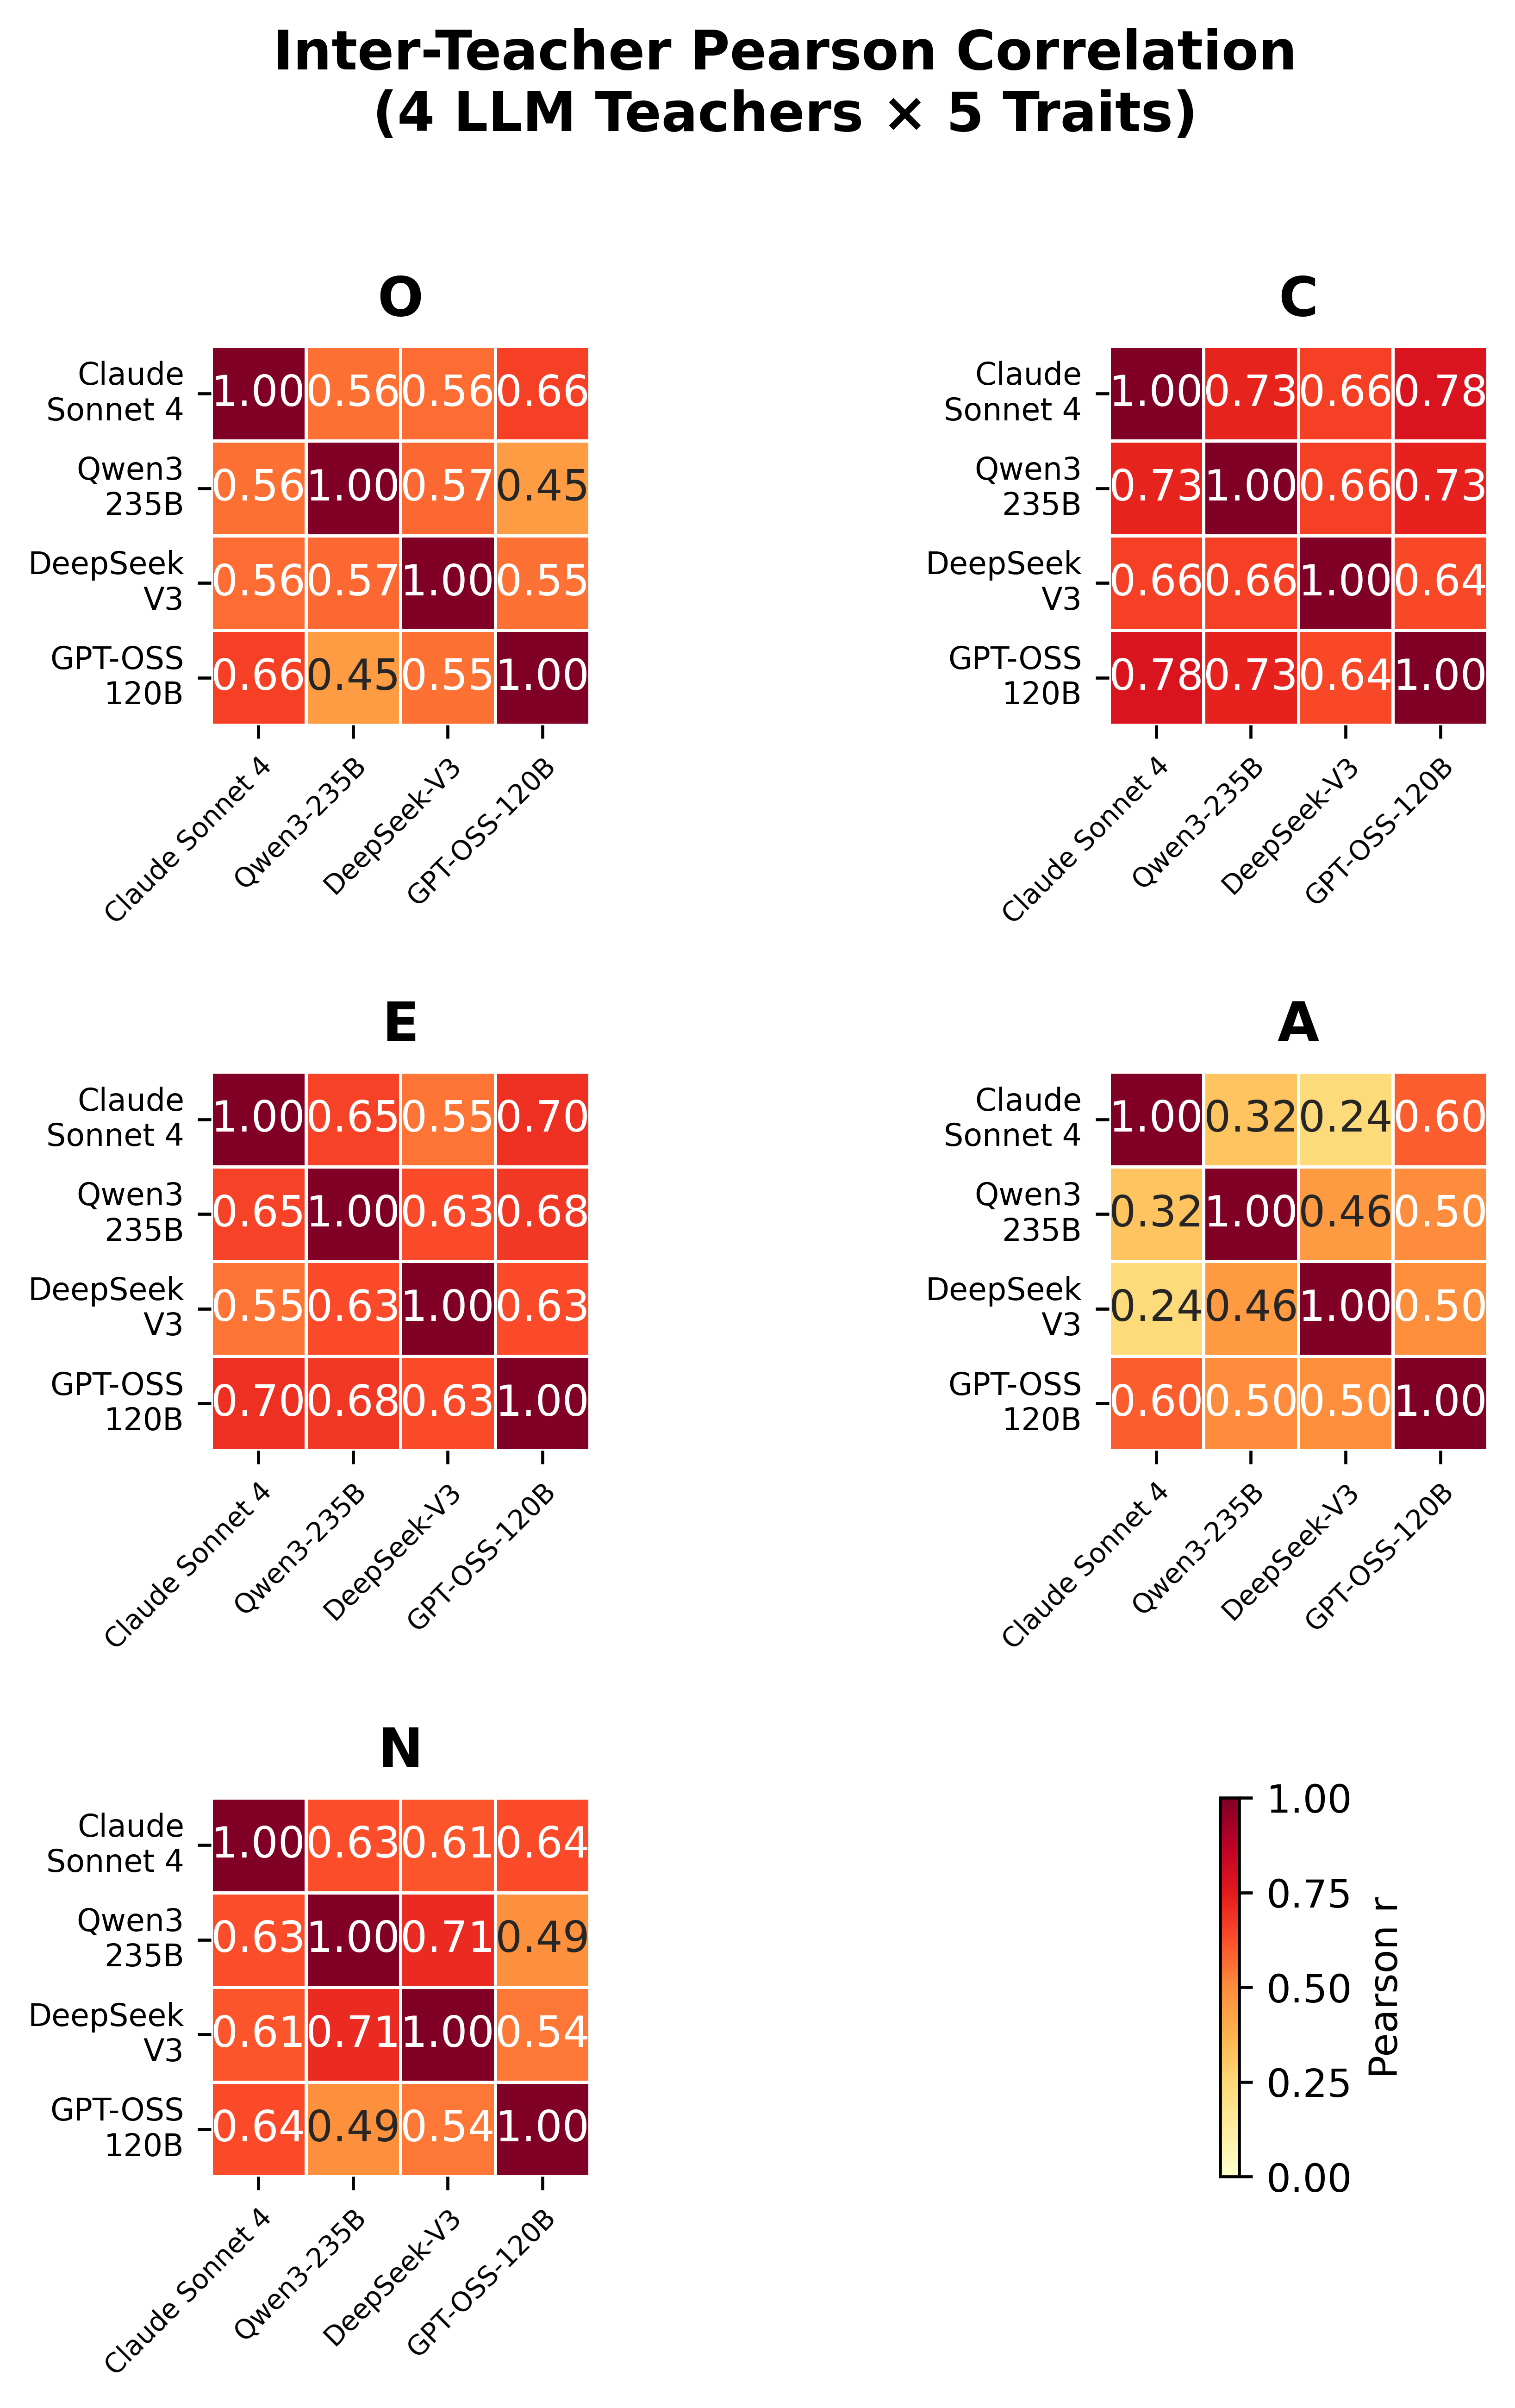
\includegraphics[width=0.85\linewidth]{fig_teacher_corr_matrix.png}
\caption{モデル間一致度．
各パネルは1つのBig5次元（O, C, E, A, N）に対応し，
セル値は同一会話$\times$話者ペアに対するモデルペア間のPearson相関係数を示す．}
\label{fig:teacher_corr_matrix_appendix}
\end{figure}


\begin{figure}[htbp]
\centering
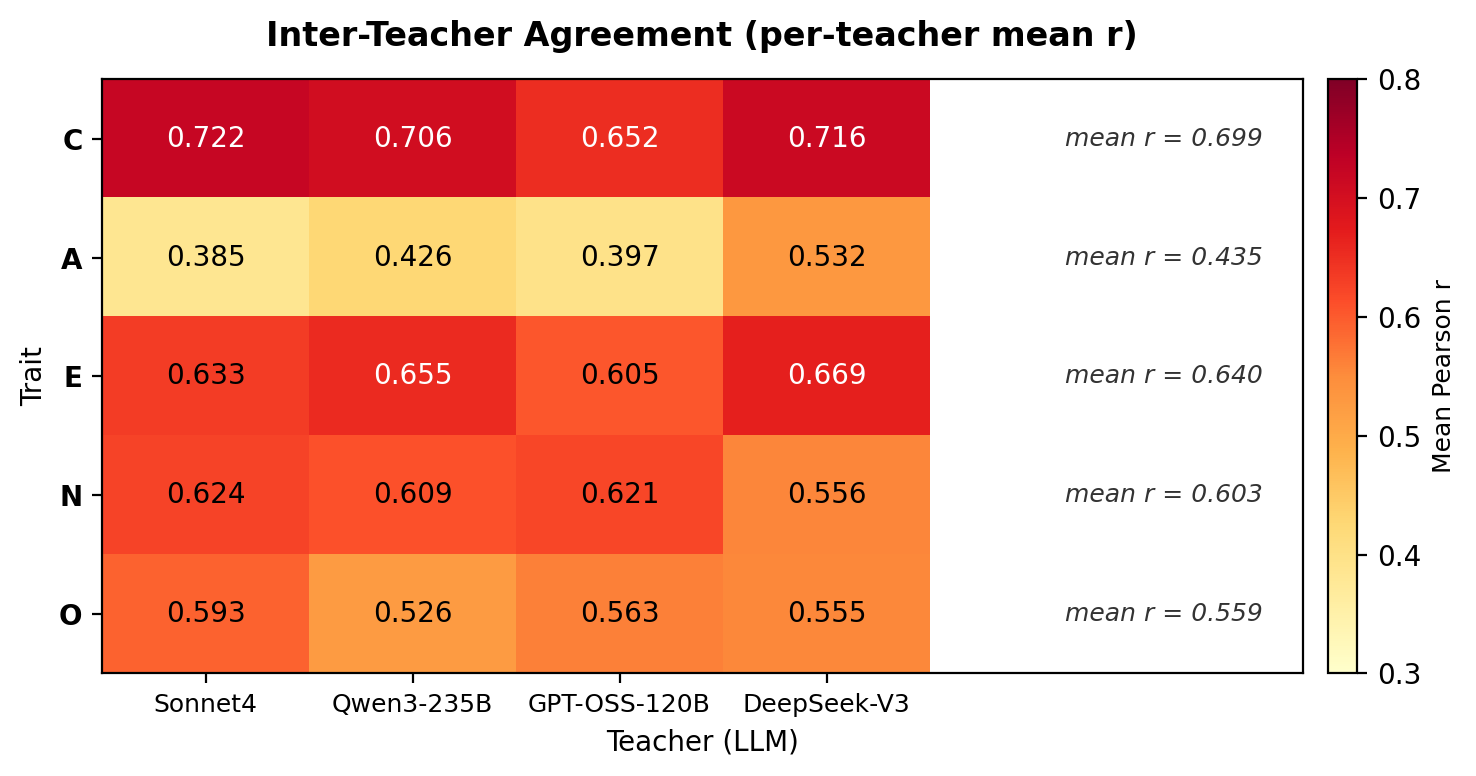
\includegraphics[width=0.9\linewidth]{fig_teacher_heatmap.png}
\caption{モデル間一致度の平均．
左側のヒートマップの各セルはペアとなるLLMモデルを平均したPearson相関係数である．さらにこの値を平均をしモデルによる影響を均した値が右側に示されている．}
\label{fig:teacher_heatmap}
\end{figure}

% [NOTE] このセクションでも頑健性に関する考察がありましたが，回帰分析の重複が多いため，回帰分析の考察と合流させるのが良いと思い移動しました．


\subsection{仮想Big5スコアの予測性能の差異}
\label{sec:appendix_individual_teacher}

% [NOTE] LLM個別の結果は感度分析のセクションとして構造を整理しました．
% [山下6/22適用] 3.4.6教師間一致度節を付録sec:appendix_teacher_agreementへ移設し、本文は1文の頑健性傍証に圧縮．
% [NOTE] 本文の3段階リッジ回帰と揃えるために，相関係数ではなくRMSEで評価するのがよいですね
% [CHECK] このセクションの結果は，C因子を特別に扱う必要はないと思いました．Cと同様に4モデル中3モデルが有意だったという例はいくつかありますので．そのため，結果の調整（例，各因子間で説明の粒度を揃える）・考察の調整（例，C因子の結果を極端に強調しすぎない）をお願いいたします．もしくはC因子が頑健であることをより明確に主張するべきです（どういった点がCが有意なのか）．

表\ref{tab:perm_all}に，個別のLLMモデルを使用してBig5スコアの推定を行った場合のリッジ回帰分析の結果を示した．

\begin{table}[htbp]
\centering
\caption{個別モデルの置換検定結果
  観測相関係数$r_{\text{obs}}$（$p$値）．$^{*}$は$p < 0.05$を示す．}
\label{tab:perm_all}
\begin{tabular}{lcccc}
\toprule
Trait & Sonnet4 & Qwen3-235B & GPT-OSS-120B & DeepSeek-V3 \\
\midrule
C & \textbf{0.360 (0.0038)} & \textbf{0.403 (0.0010)} & \textbf{0.452 (0.0006)} & 0.229 (0.0674) \\
A & 0.188 (0.1540) & \textbf{0.285 (0.0258)} & \textbf{0.394 (0.0028)} & \textbf{0.278 (0.0288)} \\
E & 0.214 (0.1004) & \textbf{0.281 (0.0314)} & 0.231 (0.0758) & 0.236 (0.0646) \\
N & 0.111 (0.3929) & \textbf{0.291 (0.0222)} & \textbf{0.539 (0.0002)} & \textbf{0.267 (0.0342)} \\
O & 0.239 (0.0618) & \textbf{0.315 (0.0148)} & \textbf{0.322 (0.0102)} & \textbf{0.411 (0.0008)} \\
\bottomrule
\end{tabular}

\end{table}

Cは4モデル中3モデルで有意な予測精度を示した:
Claude Sonnet 4（$r = 0.360$, $p = 0.0038$），
Qwen3-235B（$r = 0.403$, $p = 0.0010$），
GPT-OSS-120B（$r = 0.452$, $p = 0.0006$）．
DeepSeek-V3のみ有意水準に達しなかった（$r = 0.229$, $p = 0.0674$）．

Agreeableness（A）は，4モデル中3モデルで有意であった:
Qwen3-235B（$r = 0.285$, $p = 0.0258$），
GPT-OSS-120B（$r = 0.394$, $p = 0.0028$），
DeepSeek-V3（$r = 0.278$, $p = 0.0288$）．
Claude Sonnet 4のみ有意水準に達しなかった（$r = 0.188$, $p = 0.1540$）．

Openness（O）は，4モデル中3モデルで有意であった:
Qwen3-235B（$r = 0.315$, $p = 0.0148$），
GPT-OSS-120B（$r = 0.322$, $p = 0.0102$），
DeepSeek-V3（$r = 0.411$, $p = 0.0008$）．

Extraversion（E）は，4モデル中1モデルで有意であった:
Qwen3-235B（$r = 0.281$, $p = 0.0314$）．

Neuroticism（N）は，4モデル中3モデルで有意であった:
Qwen3-235B（$r = 0.291$, $p = 0.0222$），
GPT-OSS-120B（$r = 0.539$, $p = 0.0002$），
DeepSeek-V3（$r = 0.267$, $p = 0.0342$）．
Claude Sonnet 4のみ有意水準に達しなかった（$r = 0.111$, $p = 0.3929$）．

\subsection{考察}

個別LLMモデルごとの置換検定（\ref{sec:appendix_individual_teacher}，表\ref{tab:perm_all}）では，
C・A・O・Nの4次元がいずれも4モデル中3モデルで有意な予測精度を示し，
Eのみが1モデルにとどまった．
したがって「4モデル中3モデルで有意」という水準はCに固有のものではなく，
複数の性格次元に共通してみられる．
ただし，どのモデルで有意となるかは次元によって異なり
（例: CはDeepSeek-V3で，A・O・NはClaude Sonnet 4で有意水準に達しない），
個別モデルレベルの結果にはモデル依存性がある．

このモデル依存性は，モデル間一致度（\ref{sec:appendix_teacher_agreement}）と対応する．
Cは一致度が最も高く（$\bar{r} = 0.699$），4モデルが類似したスコアを付与するため，
相互行為特徴量による予測がモデル横断で最も安定する．
一方，Aは個別モデルでも3モデルで有意であり，4モデル平均（仮想Big5）での予測精度も最高だが
（$r = 0.449$），一致度は最も低く（$\bar{r} = 0.435$），
モデルの選択によって結果が変わりやすい．
すなわちCの特徴は「予測精度の高さ」そのものではなく，
モデル横断での頑健性（再現性）にある．

4モデルのitem-level平均による仮想Big5の解析では，O・C・A・Nの4次元で
有意な関連が認められ（\ref{sec:result_big5}），Eのみが非有意であった．
これは個別モデルレベルのパターン（Eの有意モデル数が最も少ない）と整合し，
平均化がA・O・Nの推定を安定化させうることを示す．
会話行動の観点では，Cに関連する行動（発話タイミング，YES/NO応答，
応答の定型性）はLLMにとって比較的観察・解釈しやすく，
Eに関連する行動は最も解釈が分かれやすいと考えられる．

なお，GPT-OSS-120Bは5次元中4次元（C・A・O・N）で有意となり，
他の3モデルより多くの次元で有意な予測を示した．
これは同モデルが特徴量全体に対して感度が高い，
あるいは次元間の分離が相対的に弱い可能性を示唆する．





\section{ベースライン検証}
\label{sec:baseline_validation}

LLMによるBig5性格推定が会話テキストの内容に基づいているのか，あるいはテキストの表層的統計量（発話量・文字数等）のみから推定しているのかを検証するため，3条件比較実験を実施した．

\subsection{方法}
\label{sec:baseline_validation_method}

比較の対象となる3条件は以下の通りである．

\begin{itemize}
  \item 条件1（テキストあり）: 会話テキスト全文をLLMに提示する．
    これは2.3節で述べた仮想モデルプロトコルと同一であり，本分析の主条件に相当する．
  \item 条件2（要約のみ）: 会話テキストの代わりに，
    発話数・平均発話長・会話全体の長さ・フィラー数の4つの基本統計量のみを
    自然言語テキストとしてLLMに提示する．
  \item 条件3（ランダムテキスト）: 同一の分析対象データ（$N = 120$）から
    無作為に選んだ別話者の会話テキストを提示する．
    すなわち，テキスト内容と話者の対応関係を意図的に崩した条件である．
\end{itemize}

条件2では，各会話$\times$話者レコードについて，発話parquetから以下の4統計量を算出した．

(a) 当該話者の発話数$n_{\text{utt}}$，
(b) 平均発話長（空白除去後の文字数の平均）$\bar{l}_{\text{chars}}$，
(c) 会話全体の長さ（秒）$d_{\text{sec}}$，
(d) フィラー数（「えっと」「えー」「あの」の合計出現数）$n_{\text{filler}}$．

これらの統計情報を「この話者は合計$n_{\text{utt}}$回発話し，平均発話長は
$\bar{l}_{\text{chars}}$文字，会話全体の長さは$d_{\text{sec}}$秒，フィラーは
$n_{\text{filler}}$回使用しました」というテンプレートに埋め込み，会話テキストの
代用とした．プロンプトテンプレート・温度パラメータ・乱数シードは条件1と同一とし
た．

条件3では，$N = 120$レコードのテキストカラムをderangement（完全順列）によりシャッ
フルした．プロンプトテンプレートは条件1と同一であり，テキスト内容のみが別話者の
ものに差し替えられている．

Derangementとは，すべての要素が元の位置とは異なる位置に配置される順列であり，各
話者に対して必ず別話者のテキストが割り当てられることを保証する．アルゴリズムとし
てFisher-Yatesシャッフル（乱数シード$= 42$）を適用し，固定点（自分自身のテキスト
が割り当てられた要素）が残った場合は隣接要素とのスワップにより解消した．シャッフ
ル前後でconversation\_id $\times$ speaker\_idの集合が同一であること，およびテキ
ストの多重集合が保存されることを検証した．

3条件それぞれについて，2.3節と同一の4モデル（Claude Sonnet 4, Qwen3-235B, DeepSeek-V3,
GPT-OSS-120B）でIPIP-NEO-120の全120項目を採点し，item-level平均による仮想Big5ス
コアを算出した．各条件の仮想Big5スコアを目的変数，相互行為特徴量を説明変数として，
2.4節と同一のRidge回帰（$\alpha = 100$，5-fold subject-wise CV）および置換検定
（$n_{\text{perm}} = 5{,}000$，Holm法による多重比較補正）を実行し，各条件
$\times$各traitの$r_{\text{obs}}$と$p$値を算出した．

% [NOTE] 本文のメイン指標(RMSE)に揃えるのが良いですね．3段階リッジの扱いがどうなるかわからないため後回しでも大丈夫です．

%\begingroup\sloppy
条件間の比較では，条件1の$r_{\text{obs}}$と条件2・条件3の$r_{\text{obs}}$の差分
$\Delta r$を算出し，$\Delta r \geq 0.1$を「条件1が優位（$\gg$）」，$\Delta r <
0.1$を「同等（$\approx$）」と判定した．

条件1 $\gg$ 条件2 $\approx$ 条件3 であれば，LLMは会話テキストの内容（相互行為パ
ターン）を利用して性格推定を行っていると解釈される．一方，条件2 $\approx$ 条件1
であれば，LLMは表層的統計量（発話量・文字数等）に依存している可能性が示唆される．

% \par\end group

\subsection{結果}
\label{sec:result_baseline}

表\ref{tab:baseline_comparison}に，3条件（条件1: テキストあり，条件2: 要約のみ，
条件3: ランダムテキスト）の仮想Big5に対する置換検定結果を示す．

%% TODO: 条件2・条件3のLLM採点完了後に実測値で更新する → 2026-04-08 更新済み
\begin{table}[htbp]
\centering
\caption{3条件比較結果．条件1（テキストあり），条件2（要約のみ），条件3（ランダムテキスト）の置換検定結果．}
\label{tab:baseline_comparison}
\begin{tabular}{llrrrrrl}
\toprule
条件 & trait & $r_{\text{obs}}$ & $p$値 & $p$値(補正後) & $\Delta r$ & 判定 \\
\midrule
%% --- 条件1（テキストあり）: 3.4.1節の既存結果を転記 ---
条件1 & O & 0.410 & 0.0014 & 0.0042 & --- & --- \\
条件1 & C & 0.432 & 0.0006 & 0.0024 & --- & --- \\
条件1 & E & 0.234 & 0.0658 & 0.0658 & --- & --- \\
条件1 & A & 0.449 & 0.0004 & 0.0020 & --- & --- \\
条件1 & N & 0.317 & 0.0122 & 0.0244 & --- & --- \\
\midrule
%% --- 条件2（要約のみ）---
条件2 & O & 0.528 & 0.0002 & 0.0010 & $-0.118$ & テキスト内容依存 \\
条件2 & C & 0.640 & 0.0002 & 0.0010 & $-0.208$ & テキスト内容依存 \\
条件2 & E & 0.302 & 0.0170 & 0.0170 & $-0.068$ & 表層統計量依存の可能性 \\
条件2 & A & 0.374 & 0.0036 & 0.0072 & $+0.075$ & 表層統計量依存の可能性 \\
条件2 & N & 0.711 & 0.0002 & 0.0010 & $-0.394$ & テキスト内容依存 \\
\midrule
%% --- 条件3（ランダムテキスト）---
条件3 & O & 0.161 & 0.2134 & 0.8536 & $+0.249$ & テキスト内容依存 \\
条件3 & C & $-0.080$ & 0.5463 & 1.0000 & $+0.512$ & テキスト内容依存 \\
条件3 & E & $-0.072$ & 0.5859 & 1.0000 & $+0.306$ & 表層統計量依存の可能性 \\
条件3 & A & 0.071 & 0.5981 & 1.0000 & $+0.378$ & 表層統計量依存の可能性 \\
条件3 & N & $-0.280$ & 0.0280 & 0.1400 & $+0.597$ & テキスト内容依存 \\
\bottomrule
\end{tabular}
\end{table}

条件1（テキストあり）では，3.4.1節で報告した通り，
Eを除く4次元（O, C, A, N）で有意な予測精度が認められた．
条件3（ランダムテキスト）では，全5次元でHolm補正後に有意水準に達せず
（$r_{\text{obs}} = -0.280$〜$0.161$，$p_{\text{corrected}} \geq 0.14$），
テキストと話者の対応関係を崩すと予測力が完全に消失することが確認された．
これは条件3が陰性対照として適切に機能していることを示す．

条件2（要約のみ）では，予想に反して全5次元で有意な$r_{\text{obs}}$が得られた
（$r = 0.302$〜$0.711$，$p_{\text{corrected}} \leq 0.017$）．
特にN（$r = 0.711$）およびC（$r = 0.640$）は条件1を上回る$r_{\text{obs}}$を示した．
ただし，条件2のCronbach's $\alpha$は全モデル・全次元で著しく低く
（4モデル平均: O $= 0.063$, C $= 0.176$, E $= 0.041$, A $= 0.194$, N $= 0.298$），
条件1（$\alpha \geq 0.78$）と比較してLLMの回答の内的一貫性が大幅に低下している．
この結果は，条件2のLLMスコアが項目間で一貫した性格像を反映していないにもかかわらず，
相互行為特徴量との相関が検出されたことを意味する．
この解釈については4.6節で詳述する．

\subsection{考察}
\label{sec:discuss_baseline}

%% 2026-04-08 実測値に基づいて更新済み

3.5節で報告したベースライン検証の結果は，
本研究の循環的枠組み——「説明可能な特徴量→ブラックボックスLLM→説明可能な特徴量に戻る」
（1節参照）——の妥当性を評価する上で重要な知見を提供する．
条件1（テキストあり）の$r_{\text{obs}}$が条件2（要約のみ）・条件3（ランダムテキスト）に対して
十分に高い場合（$\Delta r \geq 0.1$），
LLMは会話テキストの内容——すなわち相互行為パターン——を利用して性格推定を行っていると解釈され，
本研究が採用する「LLMで推定→古典特徴量で解釈」という枠組みの前提が支持される．
この場合，3.4節で同定されたCの寄与特徴量（発話率，沈黙系指標，YES/NO応答率等）は，
LLMが実際にテキスト内容から読み取った情報と整合する解釈可能な指標として位置づけられる．

一方，条件2の$r_{\text{obs}}$が条件1と同等（$\Delta r < 0.1$）である場合，
LLMは会話テキストの内容よりも表層的統計量（発話量・文字数等）に依存して
性格推定を行っている可能性が示唆される．
この結果は本研究の枠組みにとって限界を示すものであるが，
同時に興味深い知見でもある．
すなわち，発話数や平均発話長といった基本統計量のみからでも
性格特性との関連が検出されるならば，
これらの表層的特徴自体が性格の行動的表出を反映している可能性がある．
この場合，提案特徴量のうちPG系（タイミング）やFILL系（フィラー）の指標は
表層統計量と部分的に重複する情報を捉えている一方，
IX系（連鎖組織）やRESP系（応答型）の指標が
表層統計量では捉えきれない独自の情報を提供しているかどうかが，
3段階Ridge回帰比較（3.4.3節）のStage 2→3の増分（$\Delta R^2$）と合わせて検討すべき論点となる．

条件3（ランダムテキスト）は陰性対照（negative control）として機能する．
テキスト内容と話者の対応関係を意図的に崩した条件3において
$r_{\text{obs}} \approx 0$（有意でない）であれば，
LLMの性格推定がテキストと話者の対応関係に依存していることが確認される．
逆に，条件3でも一定の$r_{\text{obs}}$が観測される場合，
LLMがテキスト内容ではなくプロンプトの構造的特徴や
回答バイアスに基づいて推定している可能性を示唆し，
仮想モデルプロトコル（2.3節）の妥当性に対する注意喚起となる．


\section{Dose-Response実験}

本研究では，LLMを「仮想モデル」としてBig5スコアを推定し，
その推定値を外部基準として相互行為特徴量の妥当性を検証した．
この枠組みにおいて自然に生じる問いは，
LLMは性格特性を推定する際に，本研究が提案する特徴量に実際に着目しているのか
という点である．

この問いに対して，本研究ではFeature Dose-Response実験を設計・実施した．
具体的には，CEJC実データ（$N = 120$）の会話テキスト中のフィラー率を
3段階で操作（×0: 全削除，×1: 元データ，×3: 3倍）し，
LLMのCスコア推定が対応して変化するかを検証する．


\subsection{方法}
操作対象としてFILL\_rate\_per\_100chars（100文字あたりフィラー率）を選定した．
選定理由は以下の3点である:
(1) Permutation回帰係数検定およびBootstrap分散分析の両方で
Cの安定的な寄与特徴量として同定されていること（3.4.4--3.4.5節），
(2) Bootstrap topk\_rateが4モデル中3モデルで0.49以上と高いこと，
(3) 対話テキスト上でフィラー（えっと，えー，あの）の挿入・削除が
明確に操作可能であること．
対象traitとしてConscientiousness（C）を選定した．
Cは4モデル中3モデルで有意な予測精度を示し（3.4.2節），
モデル間一致度も$\bar{r} = 0.699$と5次元中最も高く（\ref{sec:appendix_teacher_agreement}），
モデル横断での頑健性において最も優れているためである．
他のtraitへの拡張は今後の課題とする．


本検証は以下の手順で構成される．
(1) CEJC実データ（$N = 120$）の会話テキストに対して，
フィラーを3段階で操作した条件別テキストを生成する．
×0条件ではフィラーの全てを等長の中立的接続詞（例: 「えっと」→「それで」，
「あの」→「その」）で置換し，テキスト長を保存する．
×1条件は元データをそのまま使用する（ベースライン）．
×3条件では既存発話内の自然な位置（文頭，読点の後）にフィラーを追加し，
フィラー出現数を元の約3倍にする．
全条件でテキストの総文字数を元テキストの$\pm 5\%$以内に保ち，
発話数（行数）は変更しない．
これにより，テキスト長や発話量の変化がLLM推定に与える交絡効果（Volume Bias）を排除する．
(2) 各条件のテキストに対して，2.3節と同一の仮想モデルプロトコル
（4モデルitem-level平均＝仮想Big5，IPIP-NEO-120のC24項目）でCスコアを推定する．
(3) 各条件のCスコアを比較し，用量反応関係の有無を評価する．
FILL\_rate\_per\_100charsのCに対する回帰係数は正であるため，
×0 $<$ ×1 $<$ ×3 の順でCスコアが単調増加する傾向が予測される．

3段階（×0, ×1, ×3）とした理由は，CEJCデータのフィラー数中央値が13.5個と少なく，
×0.5と×2.0では操作量の差が不十分なためである．
×0（全削除: 0個）で明確な下限を，×3（3倍: 中央値話者で約40個）で
十分な上限を確保した．

\subsection{結果}

4モデルitem-level平均（仮想Big5）によるDose-Response実験の結果，
フィラー率の操作によるCスコアの有意な変化は検出されなかった．
×0条件（フィラー全削除）の仮想Cスコア（4モデル平均）は$\bar{C}_{{\times 0}} = 2.227$，
×3条件（フィラー3倍）は$\bar{C}_{{\times 3}} = 2.215$であり，
$\Delta C = -0.012$（スケール0--4の0.3\%）と実質的にゼロであった．
モデル別に見ても，Claude Sonnet 4（$\Delta C = -0.003$），Qwen3-235B（$\Delta C = -0.023$），
DeepSeek-V3（$\Delta C = -0.023$），GPT-OSS-120B（$\Delta C = 0.000$）と，
いずれのモデルでもフィラー操作によるCスコアの変化は検出されなかった．
話者レベルでは，120名中51名でCスコアが上昇，63名で下降，6名で不変であり，
一貫した方向性は認められなかった．

この結果は，フィラー率がRidge回帰においてCの有意な寄与特徴量として
同定された（3.4.4--3.4.5節）にもかかわらず，
フィラーの機械的な操作ではCスコアが変化しないことを示す．
すなわち，フィラー率はCの「指標」（相関的関連因子）ではあるが，
LLMの性格推定における「原因」（因果的決定因子）ではない可能性が高い．
フィラー率が高い話者は，同時に他の相互行為パターン
（発話の計画性，応答の丁寧さ，会話の構造化等）も持っており，
LLMはフィラーの数ではなく，これらの共変動する会話全体の相互行為パターンを
総合的に評価していると考えられる．
この知見は，Transformerのself-attention機構が
個別のフィラートークンよりも会話全体の文脈構造に注目している可能性と整合する．

\subsection{限界}
ただし，本検証にはいくつかの重要な限界がある．
第一に，テキスト操作（フィラーの等長置換・挿入）は対話の自然さを損なう可能性がある．
フィラーの使用は発話計画過程や会話の文脈に依存しており\cite{clark1996,watanabe2003}，
文脈を無視した操作は不自然な対話を生成しうる．
第二に，フィラー操作はOIRマーカー（「えっ」等）と部分的に重複するため，
フィラー操作がOIR率に副作用を及ぼす可能性がある．
第三に，テキスト長保存制約（$\pm 5\%$以内）を課しているが，
フィラー挿入に伴う行末の文字削減が会話内容に影響する可能性がある．
第四に，本検証はフィラー率のみを対象としており，
他の寄与特徴量（YES/NO応答率，沈黙系指標等）への拡張は今後の課題である．

これらの限界を踏まえ，本検証の結果は
循環的枠組みの実現可能性の実証として位置づけられるものであり，
因果的な結論を導くものではない．
今後の研究では，(1) YES/NO応答率など他の寄与特徴量への拡張，
(2) LLMのattention weightやtoken-level寄与度を分析する説明可能AI（XAI）手法の適用，
(3) 特徴量の値が極端に異なる話者ペアを比較するnatural experiment的アプローチの採用，
(4) ASDコーパスへの同一枠組みの適用（ASD群の特徴量パターンを定型群に近づけた場合のLLM推定変化の検証），
といった方向性が考えられる．
これらの検証が蓄積されれば，「LLMで推定→古典特徴量で解釈→LLMで検証」という
本研究の循環的枠組み（1節参照）の最終段階をより強固に完成させることができ，
LLMと古典的特徴量の相互補完関係を実証的に裏付けることが可能となる．

さらに，LLMが会話テキストの内容（相互行為パターン）に基づいて性格スコアを推定しているのか，
あるいはテキストの表層的特徴（発話量，文字数等）のみから推定しているのかという問いに対して，
本研究では3条件比較によるベースライン検証を実施した（2.6節参照）．
条件1（テキストあり），条件2（要約のみ），条件3（ランダムテキスト）の
3条件でLLMによるBig5採点を実行し，条件間の予測精度を比較した結果を3.5節に報告した．
この検証は，「説明可能な特徴量→ブラックボックスLLM→説明可能な特徴量に戻る」という
本研究の循環的枠組みの妥当性を裏付ける上で不可欠な検証であり，
その考察は4.6節で詳述する．

\clearpage  % 全フロートを出力してから参考文献に進む

%% ============================================================
%%  References
%% ============================================================
\begin{thebibliography}{99}

\bibitem{hu2025}
Hu, C. B., et al. (2025).
Exploiting large language models for diagnosing autism associated language disorders and identifying distinct features.
\textit{npj Digital Medicine}, 8, Article 763.

\bibitem{wright2026}
Wright, A. G. C., Ringwald, W. R., Vize, C. E., et al. (2026).
Assessing personality using zero-shot generative AI scoring of brief open-ended text.
\textit{Nature Human Behaviour}.
\url{https://doi.org/10.1038/s41562-025-02389-x}

\bibitem{mun2024}
Mun, J., et al. (2024).
Developing an end-to-end framework for predicting the social communication severity scores of children with autism spectrum disorder.
\textit{arXiv preprint}, arXiv:2409.00158.

\bibitem{nakamura2025}
Nakamura, Y., et al. (2025).
ADOS-2会話テキストからのASD分類: BERT由来特徴量とLightGBMによる検討.
\textit{SICE東北支部研究会資料}, 353-9.

\bibitem{sacks1974}
Sacks, H., Schegloff, E. A., \& Jefferson, G. (1974).
A simplest systematics for the organization of turn-taking for conversation.
\textit{Language}, 50(4), 696--735.

\bibitem{schegloff1977}
Schegloff, E. A., Jefferson, G., \& Sacks, H. (1977).
The preference for self-correction in the organization of repair in conversation.
\textit{Language}, 53(2), 361--382.

\bibitem{levitan2012}
Levitan, R., Gravano, A., Willson, L., Beňuš, Š., Hirschberg, J., \& Nenkova, A. (2012).
Acoustic-prosodic entrainment and social behavior.
\textit{Proceedings of NAACL-HLT 2012}, 11--19.

\bibitem{deruiter2006}
De Ruiter, J. P., Mitterer, H., \& Enfield, N. J. (2006).
Projecting the end of a speaker's turn: A cognitive cornerstone of conversation.
\textit{Language}, 82(3), 515--535.

\bibitem{campione2002}
Campione, E. \& Véronis, J. (2002).
A large-scale multilingual study of silent pause duration.
\textit{Proceedings of Speech Prosody 2002}, 199--202.

\bibitem{clark1996}
Clark, H. H. (1996).
\textit{Using Language}.
Cambridge University Press.

\bibitem{watanabe2003}
Watanabe, M. (2003).
The constituent complexity and types of fillers in Japanese.
\textit{Proceedings of the 15th International Congress of Phonetic Sciences (ICPhS-15)}, 2473--2476.

\bibitem{kendrick2015}
Kendrick, K. H. (2015).
Other-initiated repair in English.
\textit{Open Linguistics}, 1(1), 164--190.

\bibitem{albert2018}
Albert, S. \& De Ruiter, J. P. (2018).
Repair: The interface between interaction and cognition.
\textit{Topics in Cognitive Science}, 10(2), 279--313.

\bibitem{brennan1996}
Brennan, S. E. \& Clark, H. H. (1996).
Conceptual pacts and lexical choice in conversation.
\textit{Journal of Experimental Psychology: Learning, Memory, and Cognition}, 22(6), 1482--1493.

\bibitem{kita2007}
Kita, S. \& Ide, S. (2007).
Nodding, aizuchi, and final particles in Japanese conversation: How conversation reflects the ideology of communication and social relationships.
\textit{Journal of Pragmatics}, 39(7), 1242--1254.

\bibitem{holm1979}
Holm, S. (1979).
A simple sequentially rejective multiple test procedure.
\textit{Scandinavian Journal of Statistics}, 6(2), 65--70.

\bibitem{wehrle2024}
Wehrle, S., Vogeley, K., \& Grice, M. (2024).
Backchannels in conversations between autistic adults are less frequent and less diverse prosodically and lexically.
\textit{Language and Cognition}, 16(1), 108--133.

\bibitem{leaper2007}
Leaper, C. \& Ayres, M. M. (2007).
A meta-analytic review of gender variations in adults' language use: Talkativeness, affiliative, and assertive speech.
\textit{Personality and Social Psychology Review}, 11(4), 328--363.

\bibitem{bortfeld2001}
Bortfeld, H., Leon, S. D., Bloom, J. E., Schober, M. F., \& Brennan, S. E. (2001).
Disfluency rates in conversation: Effects of age, relationship, topic, role, and gender.
\textit{Language and Speech}, 44(2), 123--147.

\bibitem{horton2010}
Horton, W. S., Spieler, D. H., \& Shriberg, E. (2010).
A corpus analysis of patterns of age-related change in conversational speech.
\textit{Psychology and Aging}, 25(3), 708--713.

\end{thebibliography}

\end{document}
